%\documentclass[pre,aps,amsmath,amssymb,amsfonts,floatfix,superscriptaddress,nofootinbib]{revtex4-1}
%\documentclass{book}

\documentclass[
12pt, % The default document font size, options: 10pt, 11pt, 12pt
%oneside, % Two side (alternating margins) for binding by default, uncomment to switch to one side
english, % ngerman for German
singlespacing, % Single line spacing, alternatives: onehalfspacing or doublespacing
%draft, % Uncomment to enable draft mode (no pictures, no links, overfull hboxes indicated)
%nolistspacing, % If the document is onehalfspacing or doublespacing, uncomment this to set spacing in lists to single
liststotoc, % Uncomment to add the list of figures/tables/etc to the table of contents
%toctotoc, % Uncomment to add the main table of contents to the table of contents
%parskip, % Uncomment to add space between paragraphs
%nohyperref, % Uncomment to not load the hyperref package
headsepline, % Uncomment to get a line under the header
%chapterinoneline, % Uncomment to place the chapter title next to the number on one line
%consistentlayout, % Uncomment to change the layout of the declaration, abstract and acknowledgements pages to match the default layout
]{MastersDoctoralThesis} % The class file specifying the document structure

\usepackage[percent]{overpic}

\usepackage{everyshi}
\usepackage{marginnote}
\usepackage{layout}
\usepackage{graphicx}
\usepackage{color}
%\usepackage{bbm}
\usepackage[utf8]{inputenc}
%\usepackage{ngerman}
\usepackage[T1]{fontenc}
\usepackage{dcolumn}
\usepackage{hyperref}
\usepackage{textcomp}
\usepackage{enumitem}
\usepackage{braket}
\usepackage{makecell}
\usepackage{wrapfig}
\usepackage{array}
\usepackage{fancyvrb}
\usepackage{multirow}
\makeatletter
\newcommand*\bigcdot{\mathpalette\bigcdot@{.5}}
\newcommand*\bigcdot@[2]{\mathbin{\vcenter{\hbox{\scalebox{#2}{$\m@th#1\bullet$}}}}}
\makeatother

%\usepackage[ngerman,english]{babel}
%\usepackage[backend=bibtex,natbib=true]{biblatex} % Use the bibtex backend with the authoryear citation style (which resembles APA)
%\usepackage[backend=bibtex,style=authoryear,natbib=true]{biblatex} % Use the bibtex backend with the authoryear citation style (which resembles APA)
%\usepackage[backend=bibtex,style=authoryear,natbib=true]{biblatex} % Use the bibtex backend with the authoryear citation style (which resembles APA)
\usepackage[maxbibnames=99,backend=biber,style=numeric,natbib=true]{biblatex} % Use the bibtex backend with the authoryear citation style (which resembles APA)
\makeatletter
\DeclareCiteCommand{\fullcite}
{\defcounter{maxnames}{\blx@maxbibnames}%
\usebibmacro{prenote}}
{\usedriver
{\DeclareNameAlias{sortname}{default}}
{\thefield{entrytype}}}
{\multicitedelim}
{\usebibmacro{postnote}}
\DeclareCiteCommand{\footfullcite}[\mkbibfootnote]
{\defcounter{maxnames}{\blx@maxbibnames}%
\usebibmacro{prenote}}
{\usedriver
{\DeclareNameAlias{sortname}{default}}
{\thefield{entrytype}}}
{\multicitedelim}
{\usebibmacro{postnote}}
\makeatother


%\usepackage{biblatex} % Use the bibtex backend with the authoryear citation style (which resembles APA)
\addbibresource{main.bib}
\usepackage[autostyle=true]{csquotes} % Required to generate language-dependent quotes in the bibliography

%\usepackage{amsfonts}
\usepackage{amssymb}
\usepackage{amsmath}
%\usepackage{lipsum}
%\usepackage{txfonts}
\numberwithin{equation}{section}
\usepackage{placeins}
\usepackage{comment}
%\usepackage[dvipsnames]{xcolor}
\usepackage{tikz}
\usetikzlibrary{calc}
\usetikzlibrary{decorations.pathmorphing}
\usetikzlibrary{decorations.pathreplacing}
\usetikzlibrary{decorations.markings}
\usetikzlibrary{shapes.misc}
\usetikzlibrary{positioning}
\usetikzlibrary{snakes}
\usetikzlibrary{arrows}
%%%%%MY%%%%


%\usepackage{graphicx}
\usepackage{graphicx}
\newcommand{\XY}[1]{\textcolor{magenta}{X$\rightarrow$ Y: #1}}
\usepackage{mathrsfs,bbm}
\usepackage{comment}
\newcommand{\bm}[1]{\boldsymbol #1}
\newcommand{\lh}{\mbox{$\neg$}}
\newcommand{\rh}{\reflectbox{$\neg$}}
\DeclareSymbolFont{symbols}{OMS}{cmsy}{m}{n}
\DeclareSymbolFont{largesymbols}{OMX}{cmex}{m}{n}

%%%%%%%%%%%%%%%%%%%%%%%%%%%%%%%%%%%%%%%%%%%%%%%%
%Contour calculus notation
\newcommand{\CS}{\mathcal{S}}
\newcommand{\ii}{^j}
\newcommand{\delC}{\delta_\CC}
\newcommand{\intC}{\int_\CC}
\newcommand{\tmin}{t_{\text{min}}}
\newcommand{\tmax}{t_{\text{max}}}
\newcommand{\CC}{\mathcal{C}}
\newcommand{\TC}{\mathcal{T}_{\CC}}
\newcommand{\gtrc}{\succ}
\newcommand{\lesc}{\prec}
%%%%%%%%%%%%%%%%%%%%%%%%%%%%%%%%%%%%%%%%%%%%%%%%
%Keldysh Green functions
\newcommand{\convz}{\ast}
\newcommand{\convi}{\bullet}
\newcommand{\convr}{\circ}
\newcommand{\ret}{{\text{R}}}
\newcommand{\adv}{{\text{A}}}
\newcommand{\mat}{{\text{\tiny M}}}
\newcommand{\tv}{{\makebox{$\neg$}}}
\newcommand{\vt}{{\reflectbox{$\neg$}}}
\newcommand{\les}{<}
\newcommand{\lar}{>}
%%%%%%%%%%%%%%%%%%%%%%%%%%%%%%%%%%%%%%%%%%%%%%%%

%\usetikzlibrary{decorations.pathreplacing,decorations.markings,snakes}
\tikzset{snake it/.style={decorate, decoration=snake}}


\usetikzlibrary{3d}
\usepackage{mathtools}
%\usetikzlibrary{arrows.meta}
    \tikzset{
            partial ellipse/.style args={#1:#2:#3}{
                        insert path={+ (#1:#3) arc (#1:#2:#3)}
                            }
                        }

\usetikzlibrary{calc}
\tikzset{
      %> = {stealth},
        % specifying distances in cm puts them in the paper coordinates,
          % without units puts them in these tikz xy(z) coordinates
            inertial frame/.style = {x={(-20:2cm)}, y={(-160:2cm)}, z={(90:2cm)}},
              local frame/.style = {shift={(local origin)}, x={(40:.7cm)}, y={(150:.7cm)}, z={(105:.7cm)}}
          }



    \tikzset{middlearrow/.style={
                decoration={markings,
                            mark= at position 0.5 with {\arrow{#1}} ,
                                    },
                                            postaction={decorate}
                                                }
                                                }
\tikzset{cross/.style={cross out, draw, 
         minimum size=2*(#1-\pgflinewidth), 
                  inner sep=0pt, outer sep=0pt}}
\hypersetup{colorlinks=true,breaklinks,linkcolor=blue,urlcolor=blue,citecolor=blue}

\newcolumntype{L}{>{$}l<{$}}

\setcounter{secnumdepth}{3}
%\renewcommand{\thechapter}{\arabic{section}}
\renewcommand{\thesection}{\Alph{section}}
\renewcommand{\theparagraph}{\textbf{§\arabic{paragraph}}}
\renewcommand{\thesubsubsection}{}
\newcommand{\und}[1]{\ensuremath{\underline{#1}}}
\renewcommand{\i}{{\ensuremath{i}}}
\newcommand{\vect}[1]{\boldsymbol{#1}}
%\newcommand{\tr}[1]{\ensuremath{\text{Tr}\left( #1 \right)}}
\newcommand{\kv}{\ensuremath{\mathbf{k}}}
\newcommand{\qv}{\ensuremath{\mathbf{q}}}
\newcommand{\Qv}{\ensuremath{\mathbf{Q}}}
\newcommand{\pv}{\ensuremath{\mathbf{p}}}
\newcommand{\av}[1]{\ensuremath{\left\langle #1 \right\rangle}}
%\newcommand{\up}{\ensuremath{\uparrow}}
\newcommand{\dn}{\ensuremath{\downarrow}}
%\newcommand{\ket}[1]{\ensuremath{\left| #1\right\rangle}}
\newcommand{\impav}[1]{\ensuremath{\left\langle #1 \right\rangle^{\text{imp}}}}
\newcommand{\rv}{\ensuremath{\mathbf{r}}} 
\newcommand{\Rv}{\ensuremath{\mathbf{R}}} 
\newcommand{\dv}{\ensuremath{\boldsymbol{\delta}}} 
\newcommand{\Ttau}{\ensuremath{T_{\tau}}}
\newcommand{\vc}[1]{\ensuremath{\mathbf{#1}}}
\newcommand{\ketvac}{\ensuremath{|0\rangle}}
\newcommand{\ketup}{\ensuremath{|\uparrow\rangle}}
\newcommand{\ketdn}{\ensuremath{|\downarrow\rangle}}
\newcommand{\ketud}{\ensuremath{|\updownarrow\rangle}}
\newcommand{\ketsig}{\ensuremath{|\sigma\rangle}}
\newcommand{\ketmsig}{\ensuremath{|\bar{\sigma}\rangle}}
\newcommand{\bravac}{\ensuremath{\langle 0|}}
\newcommand{\braup}{\ensuremath{\langle\uparrow|}}
\newcommand{\bradn}{\ensuremath{\langle\downarrow|}}
\newcommand{\braud}{\ensuremath{\langle\updownarrow|}}
\newcommand{\brasig}{\ensuremath{\langle\sigma|}}
\newcommand{\bramsig}{\ensuremath{\langle\bar{\sigma}|}}
\newcommand{\rguideqp}{\marginpar{\vspace{.4em}\textbf{\textit{\textcolor{green}{Q}}\textit{\textcolor{red}{P}}}}}
\newcommand{\rguideq}{\marginpar{\vspace{.4em}\textbf{\textit{\textcolor{green}{Q}}}}}
\newcommand{\rguidep}{\marginpar{\vspace{.4em}\textbf{\textit{\textcolor{red}{P}}}}}
\newcommand{\greenq}{\textbf{\textit{\textcolor{green}{Q}}}}
\newcommand{\redp}{\textbf{\textit{\textcolor{red}{P}}}}
\newcommand{\toclink}{\addtocontents{toc}{\protect\hypertarget{sec:\thechapter\thesection}{}}}
\newcommand{\toclinksub}{\addtocontents{toc}{\protect\hypertarget{ssec:\thechapter\thesubsection}{}}}


\def \Im {\mathop {\rm Im}}
\newcommand{\chiimp}{\ensuremath{\chi^{\text{imp}}}}
\newcommand{\Xch}{\ensuremath{X^{\text{ch}}}}
\newcommand{\Xsz}{\ensuremath{X^{\text{sz}}}}
\newcommand{\EvL}[1]{{\color{red}#1}}
\newcommand{\FJK}[1]{{\color{WildStrawberry}#1}}
\newcommand{\HH}[1]{{\color{blue}#1}}

\newcommand{\hint}{\ensuremath{H_{\text{int}}}}
\newcommand{\iom}{{\ensuremath{\i\omega}}}
\newcommand{\inu}{{\ensuremath{\i\nu}}}
\newcommand{\msigma}{{\ensuremath{\bar{\sigma}}}}
\newcommand{\RV}{\ensuremath{\mathbf{R}}}
\newcommand{\ev}{\ensuremath{\mathbf{e}}}
\newcommand{\Av}{\ensuremath{\mathbf{A}}}
\newcommand{\jv}{\ensuremath{\mathbf{j}}}
\newcommand{\abs}[1]{\ensuremath{\lvert#1\rvert}}
\newcommand{\dtau}{{\ensuremath{\partial_\tau}}}
\newcommand{\um}{\ensuremath{\mathbbm{1}}}
\newcommand{\cdag}{{\ensuremath{\mathop{c^{\dagger}}}}}
\newcommand{\tti}{\ensuremath{\tilde{t}}}
%\usepackage{showlabels}
\newcolumntype{C}[1]{>{\centering\arraybackslash}p{#1}}

\thesistitle{Ultrafast dynamics of strongly correlated systems} % Your thesis title, this is used in the title and abstract, print it elsewhere with \ttitle
%\supervisor{Dr. James \textsc{Smith}} % Your supervisor's name, this is used in the title page, print it elsewhere with \supname
\examiner{} % Your examiner's name, this is not currently used anywhere in the template, print it elsewhere with \examname
\degree{Doctor of Philosophy} % Your degree name, this is used in the title page and abstract, print it elsewhere with \degreename
\author{Viktor \textsc{Valmispild}} % Your name, this is used in the title page and abstract, print it elsewhere with \authorname
\addresses{} % Your address, this is not currently used anywhere in the template, print it elsewhere with \addressname

%\subject{Biological Sciences} % Your subject area, this is not currently used anywhere in the template, print it elsewhere with \subjectname
\keywords{} % Keywords for your thesis, this is not currently used anywhere in the template, print it elsewhere with \keywordnames
\university{Universität Hamburg} % Your university's name and URL, this is used in the title page and abstract, print it elsewhere with \univname

\AtBeginDocument{
\hypersetup{pdftitle=\ttitle} % Set the PDF's title to your title
\hypersetup{pdfauthor=\authorname} % Set the PDF's author to your name
\hypersetup{pdfkeywords=\keywordnames} % Set the PDF's keywords to your keywords
}

\begin{document}
\EveryShipout{%
      \ifthenelse{\isodd{\value{page}}}%
          {\global\marginparsep=-3cm}% Next page is even
              {\global\marginparsep=.8cm}% Next page is odd
              }
%titlepage
\frontmatter % Use roman page numbering style (i, ii, iii, iv...) for the pre-content pages
\pagestyle{plain} % Default to the plain heading style until the thesis style is called for the body content
\begin{titlepage}
\begin{center}

\HRule \\[0.4cm] % Horizontal line
{\huge \bfseries \ttitle\par}\vspace{0.4cm} % Thesis title
\HRule \\[1.5cm] % Horizontal line
\vfill

\Large \textit{Dissertation\\~\\zur Erlangung des Doktorgrades\\~\\des Fachbereichs Physik\\~\\der Universität Hamburg}\\[0.3cm] % University requirement text
    \vspace{1cm} 
    
%%%%My    %%%%%%%%%%%%%%
\vfill
\Large vorgelegt von\\
\authorname\\
%aus Münster in Westfalen
%%%%%%%%%%%%%%%%%

    \vspace{1cm} 
\Large Hamburg 2019
 
\vfill
\end{center}
\end{titlepage}

\vspace*{5cm}
\begin{minipage}{0.43\linewidth}
Gutachter der Dissertation: \\
\, \\
\end{minipage}
\begin{minipage}{1\linewidth}
Prof. Dr. Alexander I. Lichtenstein \\
Dr. Frank Lechermann \\
\end{minipage}
\vspace{1cm}


\begin{minipage}{0.43\linewidth}
Zusammensetzung der \\
Prüfungskommission: 
\, \\
\, \\
\, \\
\, \\
\, \\
\, \\
\end{minipage}
\begin{minipage}{1\linewidth}
Prof. Dr. Alexander I. Lichtenstein \\
Dr. Frank Lechermann \\
Prof. Dr. Michael Potthoff \\
Prof. Dr. Daniela Pfannkuche \\
Dr. Kirsten von Bergmann \\
\end{minipage}




\vspace{1cm}

\begin{minipage}{0.43\linewidth}
Vorsitzende der \\
Prüfungskommission:
\, \\
\end{minipage}
\begin{minipage}{1\linewidth}
Prof. Dr. Daniela Pfannkuche
\end{minipage}

\vspace{1cm}

\begin{minipage}{0.43\linewidth}
Datum der Disputation: 
\end{minipage}
\begin{minipage}{1\linewidth}
(offen)
\end{minipage}


\vspace{1cm}

\begin{minipage}{0.43\linewidth}
Vorsitzender Fach-\\
Promotionsausschusses Physik: \\
\end{minipage}
\begin{minipage}{1\linewidth}
Prof. Dr. Günter H.W. Sigl
\end{minipage}

\begin{minipage}{0.43\linewidth}
Leiter des Fachbereichs Physik: \\
\end{minipage}
\begin{minipage}{1\linewidth}
Prof. Dr. Wolfgang Hansen
\, \\
\end{minipage}

\vspace{1cm}
\begin{minipage}{0.43\linewidth}
Dekan der Fakultät MIN: \\
\end{minipage}
\begin{minipage}{1\linewidth}
Prof. Dr. Heinrich Graener
\, \\
\end{minipage}


%Prof. Dr. Wolfgang Hansen

\cleardoublepage

%----------------------------------------------------------------------------------------
%	QUOTATION PAGE
%----------------------------------------------------------------------------------------

%\vspace*{0.2\textheight}

%\noindent\enquote{\itshape Warum plagen wir einer den andern?\\ Das Leben zerrinnt, und es versammelt uns nur einmal wie heute die Zeit.}\bigbreak

%\hfill Friedrich von Schiller

\cleardoublepage
%chapters

%\pagenumbering{arabic}


%\vspace*{4cm}




%\title{\Large Conserving dynamical mean-field approaches\\to strongly correlated systems\\[4cm]\leavevmode\\
%\large Dissertation\\~\\zur Erlangung des Doktorgrades\\~\\des Fachbereichs Physik\\~\\der Universität Hamburg\\\vspace*{3cm}}
    
%\author{\large vorgelegt von\\Friedrich Johannes Krien\\aus Münster in Westfalen\\2018}
%\maketitle
%\newpage
%\leavevmode
%\newpage

\textbf{Zusammenfassung} In der Dissertation stelle ich eine theoretische Studie von ultraschnellen Prozessen in Systemen mit starken elektronischen Korrelationen vor, die durch Wechselstromfelder aus dem Gleichgewicht gebracht werden. 
Es wird besondere Aufmerksamkeit dem Verständnis des Verhaltens von Systemen mit starken elektronischen Korrelationen in externen Feldern zugeteilt, die bereits im Gleichgewicht reichhaltige Physik demonstriert haben.

Dabei verwende ich die Theorie des dynamischen Nichtgleichgewichtsmolekularfeldes (NE-DMFT) um die stark korrelierter Vielkörpersysteme im
externen Feld zeitaufgelöst zu simulieren.

Durch die Einstellung von Frequenz, Intensität, Polarisation und Pulsform des angelegten Feldes in einem breiten Parameterspektrum sowie durch elektronische Korrelationen erhalten wir Zugang zu einer Reihe neuer Phänomene, die in der vorliegenden Arbeit untersucht werden.

Ein solches Phänomen ist die Vorzeichenänderung der effektiven 
Coulomb~-~Wechselwirkung unter dem Einfluss von Halb-, Mono- und Mehrperiodenpulsen, 
die auf ein zweidimensionales Quadratgitter angewendet werden und kann als realistisches Modell für supraleitende Materialien mit hohem-$T_C$ verwendet werden könnten.

Dann verwende ich NE-DMFT, um das Einfangen von Elektronen in einen neuen metastabilen Zustand zu untersuchen und den Übergang der metallischen Phase zum Isolator zu demonstrieren. 
Dieser Übergang wird von einem effektiven Potential angetrieben, das durch die niederfrequente laserinduzierte Vielkörperdynamik erzeugt wird. 
Diese Phase wird als "Kramers-Henneberger-Festkörper" bezeichnet und in Analogie zum "Kramers-Henneberger-Atom", einem gebundenen elektronischen Zustand, der in einem neuen Potenzial vorliegt, welcher durch die kombinierte Wirkung des Laserfeldes und des Atomkerns erzeugt wurde, diskutiert.

Das Anlegen eines hochfrequenten externen elektrischen Feldes an ein dissipationsfreies Ein-Orbital-Hubbard-Modell  führt zu einer Änderung der Bandstruktur und der Impulsverteilung ohne signifikante Übertragung von Teilchen über das Fermi-Niveau. 
Diese elektronische topologische Modifikation führt zu einem feldinduzierten Lifshitz-Übergang.

Um schließlich einen Einblick in die Natur der magnetischer Anregungen in komplexen itineranten Magneten zu erhalten, verwende ich eine realistische zeit-abhängige Lineare-Antwort-Dichtefunktionaltheorie. 
Ich wende diese Theorie zur Analyse der räumlichen und zeitlichen Skalen von Spin-Dichte-Schwankungen in 3\emph{d} Ferromagneten an.


\newpage
~
\newpage

\textbf{Abstract} In the thesis, I present a theoretical study of ultrafast processes in systems with strong electronic correlations, driven out of equilibrium by ac fields.
The main point is understanding the behavior of a system with strong electronic correlations in the presence of external fields, besides, already reach physics demonstrated by such systems even in equilibrium case.

I use the nonequilibrium dynamical mean-field theory (NE-DMFT) as a method for time-resolved simulation of strongly correlated many-body systems driven out of equilibrium by the external field.

Tuning the applied field in a wide range of frequency, intensity, polarization, and pulse shape together with electronic correlations give us access to a number of new phenomena considered in the present thesis.

First such phenomenon is sign change of the effective Coulomb interaction under the influence of half- mono- and multi-cycle pulses adopted to a two-dimensional square lattice, which could be used as a realistic model of high-$T_C$ superconducting materials.

Then I apply NE-DMFT to study the trapping of electrons into a new metastable state, demonstrating the transition of the metallic phase to the insulator. This transition is driven by effective potential, generated by the low-frequency laser-induced many-body dynamics. This phase is called "Kramers-Henneberger solid", and it is discussed in analogy with "Kramers-Henneberger atom", bound electronic states residing in a new potential generated by the combined action of the laser field and 
the atomic core.

Applying a high-frequency external electric field to a one-orbital Hubbard model without dissipation leads to a change in the band structure and momentum distribution without significant transfer of particles above the Fermi level. This electronic topological modification leads to field-induced Lifshitz transition. 

Finally, in order to gain an insight into the nature of magnetic excitations in complex itinerant magnets, I use realistic linear response time-dependent density functional theory. I apply this theory for analysis of spatial and time scales of spin density fluctuations in 3\emph{d} ferromagnets.




%Last part of the tesis containce analyse of spatial and time scales of spin density fluctuations (SDF)

%Spatial and time scales of spin density fluctuations (SDF) were analyzed in 3\emph{d} ferromagnets using \emph{ab initio} linear response calculations of complete wavevector and energy dependence of the dynamic spin susceptibility tensor. We demonstrate that SDF are spread continuously over the entire Brillouin zone and while majority of them reside within the 3\emph{d} bandwidth, a significant amount comes from much higher energies.  The SDF spectrum is shown to have two main constituents: a minor low-energy spin wave contribution and a much larger high-energy component from more localized excitations. Using the fluctuation-dissipation theorem (FDT), the on-site spin correlator (SC) and the related effective fluctuating moment were properly evaluated and their universal dependence on the 3\emph{d} band population is further discussed.






\newpage


\tableofcontents
%   \begin{eqnarray*}
%   \begin{tikzpicture}
%       \draw[thick] (0,0) -- (16,0) -- (16,3.8) -- (0,3.8) -- cycle;
%        \draw (8,3) node {\Large Reading guide:};
%        \draw (8,2) node {\large A shortened but complete overview of the material is marked with \textbf{\textit{\textcolor{green}{Q}}}.};
%        \draw (8,1) node {\large For results related to physics, skipping technicalities, follow \textbf{\textit{\textcolor{red}{P}}}.};
%   \end{tikzpicture}
%   \end{eqnarray*}
%\setcounter{chapter}{-1}



%\chapter{{Reading guide}}
%\section[A shortened version of the material is marked with \textbf{\textit{\textcolor{green}{Q}}}]{\protect\hyperlink{sec:\thechapter\thesection}{A shortened version of the material is marked with \textbf{\textit{\textcolor{green}{Q}}}}}\toclink
%\section[For results related to physics (no technicalities) follow \textbf{\textit{\textcolor{red}{P}}}]{\protect\hyperlink{sec:\thechapter\thesection}{For results related to physics (no technicalities) follow \textbf{\textit{\textcolor{red}{P}}}}}\toclink
%\section[Click on section headers to return to the table of contents]{\protect\hyperlink{sec:\thechapter\thesection}{Click on section headers to return to the table of contents}}\toclink
\mainmatter
\pagestyle{thesis}

%\chapter{\protect\hyperlink{chap:\thechapter}{A case for the solid state}}
%\chapter{{A case for the solid state}}
%\addtocontents{toc}{\protect\hypertarget{chap:\thechapter}{}}
%\section[Foreword]{\protect\hyperlink{sec:\thechapter\thesection}{{Foreword}}}\toclink
%\addtocontents{toc}{\protect\hypertarget{sec:\thesection}{}}

%Tell a story about five nuts ...

%\section[Structure and scope~\greenq\redp]{\protect\hyperlink{sec:\thechapter\thesection}{Structure and scope}}\toclink\rguideqp  %\marginpar{\textbf{\textit{\textcolor{green}{Q}}\textit{\textcolor{red}{P}}}}[.1cm]
%This thesis is divided into five chapters ...

%\newpage
%\chapter{One- and two-particle correlation functions}\label{sec:viewpoint}
%\begin{center}\textit{"Sooft ich meine Tabakspfeife,\\
%Mit gutem Knaster angefüllt,\\
%Zur Lust und Zeitvertreib ergreife,\\
%So gibt sie mir ein Trauerbild.\\
%Und füget diese Lehre bei,\\
%Dass ich derselben ähnlich sei."}
%\end{center}

%\hspace{6cm}- J. S. Bach
%\vspace{1cm}

%\rguideq This chapter introduces the definitions and the notation used in the rest of the text.
%In the discussion of the many-body Hamiltonians the differences between the continuum and the lattice notation are highlighted.

%\section[Hamiltonians, operators, and correlation functions functions]{\protect\hyperlink{sec:\thechapter\thesection}{Hamiltonians, operators, and correlation functions functions}}\toclink
%\label{sec:hamiltonians}
%\textbf{\textit{\textcolor{green}{Q}}}
%In the continuum, one defines the Hamiltonian of a many-electron system as follows,
%\begin{align}
%H&=\sum_\sigma\int d^3r \Psi^\dagger_\sigma(\rv)\left(-\frac{\Delta_{\rv}}{2}+v(\rv)\right)\Psi_\sigma(\rv)\notag\\
%&+\frac{1}{2}\sum_{\sigma\sigma'}\int\int d^3rd^3r' \Psi^\dagger_\sigma(\rv)\Psi^\dagger_{\sigma'}(\rv')V(|\rv-\rv'|)\Psi_{\sigma'}(\rv')\Psi_{\sigma}(\rv),\label{eq:mb_field_op}
%\end{align}
%Here,
%\begin{align}
%    H_0=\sum_\sigma\int d^3r\Psi^\dagger_\sigma(\rv)\left(-\frac{\Delta_\rv}{2}+v(\rv)\right)\Psi_\sigma(\rv),
%\end{align}
%describes the kinetic motion of many non-interacting electrons in a periodic potential of static ions $v(\rv)$.
%Electrons of spin $\sigma$ are created (annihilated) at location $\rv$ by the fermionic field operators $\Psi^{(\dagger)}_\sigma(\rv)$.
%The Coulomb interaction between the electrons is denoted as
%\begin{align} 
% \hint = \frac{1}{2}\sum_{\sigma\sigma'}\int\int d^3rd^3r' \Psi^\dagger_\sigma(\rv)\Psi^\dagger_{\sigma'}(\rv')V(|\rv-\rv'|)\Psi_{\sigma'}(\rv')\Psi_{\sigma}(\rv),\label{hint}
%\end{align}
%where $V(|\rv-\rv'|)=|\rv-\rv'|^{-1}$ is the Coulomb potential.

%\subsection[Charge and spin densities of the continuum]{\protect\hyperlink{ssec:\thechapter\thesubsection}{Charge and spin densities of the continuum}}\toclinksub
%Of interest for microscopic conservation laws is the time-evolution of the electronic charges and spins.
%In the following, $n(\rv)=\sum_\sigma\Psi^\dagger_\sigma(\rv)\Psi_{\sigma}(\rv)$ denotes the charge density operator in real space. More generally, one defines the density operators,
%\begin{align}
%    \varrho^\alpha(\rv)=\sum_{\sigma\sigma'}\Psi^\dagger_\sigma(\rv)s^\alpha_{\sigma\sigma'}\Psi_{\sigma'}(\rv)\label{def:rho_cont},
%\end{align}
%where $s^\alpha_{\sigma\sigma'}$ are the Pauli matrices. With $s^c_{\sigma\sigma'}=\delta_{\sigma\sigma'}$ one recovers the charge density, $\varrho^c(\rv)=n(\rv)$,
%whereas $\alpha=x,y,z$ yield the spin density operators.
%The operators $S^\alpha=\varrho^\alpha/2$ obey the commutation relations $[S^\alpha,S^\beta]=\sum_\gamma\varepsilon_{\alpha\beta\gamma}S^\gamma$,
%and one may extend the definition of the Levi-Civita symbol to $\varepsilon_{\alpha\beta\gamma}=0$ in case one of its labels $\alpha,\beta,\gamma$ is equal to
%the charge flavor $c$.
%This reflects the fact that the charge density commutes with all other densities and itself, $[\varrho^c,\varrho^\alpha]=0$ for each $\alpha$.
%Despite the characteristic commutation relations, the spin density operators $\varrho^{x,y,z}$ are not proper spin operators, for reasons explained below.

%The above notation is most useful in absence of discrete translational symmetry, such as in the physics of liquid Helium~\cite{Vollhardt84}.
%To approach quantum lattice problems, the continuum notation is rarely used anymore,
%since it does not make use of the periodicity of the ionic potential $v(\rv+\Rv)=v(\rv)$.
%This makes the continuum picture unfavorable in numerical approaches, due to the continuous spatial variable $\rv$. 

%A particular advantage of the continuum over the lattice notation is the simplicity of the Coulomb potential, which is an interaction between charge densities.
%Such an interaction gives an energetic incentive to electrons to avoid each other in order to minimize their potential energy.
%However, the Coulomb potential does not contribute to the charge current, which reflects in the commutativity of the Coulomb potential with the charge density, $[n(\rv),\hint]=0$.
%Likewise, the Coulomb interaction does not cause spin currents either,
%\begin{align}
%    [\varrho^\alpha,\hint]=0,
%    \label{eq:coulombcommute}
%\end{align}
%for the charge and spin densities, $\alpha=c,x,y,z$.
%These commutation relations also become intuitively clear,
%considering that the operator combination $\Psi^\dagger_\sigma(\rv)\Psi^\dagger_{\sigma'}(\rv')V(|\rv-\rv'|)\Psi_{\sigma'}(\rv')\Psi_{\sigma}(\rv)$ acting on a
%Fock state $|\Psi\rangle$ annihilates and recreates two electrons at $\rv$ and $\rv'$ with spins $\sigma$ and $\sigma'$.
%Taking the double integral over the real space, this operation thus merely counts the total potential energy of the electronic
%configuration represented by $|\Psi\rangle$, but leaves the configuration itself unchanged.
%This feature of the Coulomb interaction is exclusive to the continuum notation and lost when making use of the discrete translational symmetry of the ionic lattice.


\chapter{Introduction}

%%%%%%%%%%%%%%%%%%%%%%%%%%%%%%%%%%%%%%%%%%%%%%%%%

In the last decade growth of experimental interest in the field of ultrafast time-resolved spectroscopies in solids. Where an intense
pump laser pulse is used to drive the system into highly
excited states, while another higher frequency probe pulse is used to observe a temporal evolution of the system.
The "pump-probe" technique has enabled the study of transient and relaxation processes which is crucial to understanding ultrafast phase transitions, dynamics of various excitations and many scattering phenomena. This approach has been used to explore a variety of properties in electron systems and ultracold atoms trapped in an optical lattice.

Our fundamental interest is transient nonequilibrium phenomena in strongly correlated
electron systems particular on high-$T_C$ superconductors.
In equilibrium, strong electronic correlations bring plenty of fascinating phenomena,
such as metal-to-Mott-insulator transitions or high-$T_C$ superconductivity and various magnetic phenomena.
If such interacting many-particle systems are
driven out of equilibrium, one can observe rich unexplored variety of dynamics during and
after the perturbation. This will help us to get new physical insights into the correlated system that cannot be discovered in equilibrium.

The fast developments of experimental techniques motivate the progress of theoretical methods to study correlated fermions out of equilibrium. 
Among the many approaches that have been introduced
to study correlated systems, some have already been extended out of equilibrium.
Most successful of them the Dynamical Mean-Field Theory (DMFT) \citep{RevModPhys.68.13,Kotliar} which provides the exact solution in the limit of infinite coordination. 
DMFT approximates only the spatial correlations in a mean-field manner, but accurately treats local temporal fluctuations that are important for describing
strong-correlation phenomena. 
Using Kadanoff-Baym formalism, a general formulation of the Nonequilibrium Dynamical Mean-Field Theory (NE-DMFT) \citep{PhysRevLett.97.266408} was done to describe temporal evolutions of the system from a thermal initial state.

The goal of this thesis is a theoretical investigation
of interacting many-body systems out of equilibrium by tuning the applied pump field in a wide range of frequency, intensity, polarization and pulse shape using NE-DMFT approach.

The structure of the thesis is as follows. 
In \autoref{chap:Non_mb_th}, a brief methodological overview will be given, with an emphasis on NE-DMFT approach and approximations used in it.

In \autoref{chap:pi_pulse} we investigate changing the sign of the effective Coulomb interaction under the influence of half- mono- and multi-cycle pulses. The system adopted to a two-dimensional square lattice, which could be used as a realistic model of high-$T_c$ superconducting materials.

Than in \autoref{chap:KH_solid} we will apply NE-DMFT to study the trapping of electrons into a new metastable state, demonstrating the transition of the metallic phase to the insulator. This transition is driven by effective potential, generated by the low-frequency laser-induced many-body dynamics. This phase is called "Kramers-Henneberger solid", and it is  discussed in analogy with "Kramers-Henneberger atom", bound electronic states residing in a new potential generated by the combined action of the laser field and the atomic core.

Applying high-frequency external electric field to one-orbital Hubbard model without dissipation leads to a change in the band structure and momentum distribution without significant transfer of particles above the Fermi level. This electronic topological modification leads to field-induced Lifshitz transition and will be discussed in detail in \autoref{chap:FS}. 

In the \autoref{chap:MO_FLEX} we will discuss the importance and different ways of including additional orbital degrees of freedom for an accurate description of the electronic structure of correlated materials.

Finally in order to gain an insight into the nature of magnetic excitations in complex itinerant magnets, in the \autoref{chap:TDDFT} we will discuss a brief methodological overview to realistic linear response in the framework of time-dependent density functional theory. We also apply this theory for analysis of spatial and time scales of spin density fluctuations in 3\emph{d} ferromagnets.

%%%%%%%%%%%%%%%%%%%%%%%%%%%%%%%%%%%%%%%%%%%%%%%%%%






\FloatBarrier

%\tableofcontents

\chapter{Nonequilibrium many-body theory}
\label{chap:Non_mb_th}

\section{Nonequilibrum Green's function approach}

There are different approaches to account for time dependencies in a quantum mechanical system with its advantages and disadvantages. One of the most popular is a Keldysh formalism for nonequilibrium Green's functions. Kadanoff and Baym \citep{bookKadanoff_and_Baym} introduced the concept of two real-time Green functions, thus developing the standard equilibrium (imaginary-time) formalism \citep{Abrikosov:107441} to nonequilibrium \citep{10.1063/1.1703727}. In this work, we use L-shaped Green contour functions, which were introduced by Keldysh \citep{Keldysh:1964ud} and Danilevich \citep{DANIELEWICZ1984239}. Many theoretical approaches that have been developed for the study of strongly correlated systems can be adapted for nonequilibrium systems using the Keldysh formalism.

\FloatBarrier

\subsection{Contour idea}
	
Time-dependent experimental measurements can be related with expectation values of observables $\langle{O(t)}\rangle$. An expectation value of a quantum mechanical operator $O$ at time $t$ given by 
\begin{align}
\langle O(t)\rangle
 &=
  Tr[\rho(t)O].
\label{expectation value}
\end{align}
where $\rho(t)$ is a time-dependent density matrix. 

Initial (at $t=0$) system is in a mixed state represented by a density operator
\begin{align}
\rho(0)
&=
  \frac{1}{Z}e^{-\beta H(0)},
\label{rho0}
\end{align}
where $H(t)$ - time-dependent Hamiltonian, $\beta=1/T$ is the inverse temperature, $Z={\rm Tr}\, e^{-\beta H(0)}$ is the thermal equilibrium partition function.
At $t=0$ we switch on a driving field, and the system starts to evolve from its initial state. 
A Neumann equation describes how the density operator evolves in time and has the following expression
\begin{align}
i\frac{d}{dt}\rho(t)
 &=
  [H(t),\rho(t)],
\label{von Neumann}
\end{align}
where the brackets denote a commutator. The solution for the equation can be written as 
\begin{align}
\rho(t)
&= U(t,0)\, \rho(0) \, U(0,t),
\label{formal rho}
\end{align}

where the interaction time evolution operator defined as
\begin{align}
U(t,t')
 &=
  \begin{cases}
   \vspace{.2cm}
   \displaystyle
   T \exp\left(-i\int_{t'}^t d\bar{t}\, H(\bar{t})\right) 
   & t>t'
   \\
   \displaystyle
   \bar{T} \exp\left(-i\int_{t'}^t d\bar{t}\, H(\bar{t})\right)
   & t<t'
  \end{cases}.
\label{U def}
\end{align}
Here $T$ denotes time-ordering and $\bar{T}$ anti-time-ordering operators. Operator $H(t)$ odered by operator $T$ such that the time
arguments $\bar{t}$ increase from right to left and vice versa for $\bar{T}$. The density matrix involves one exponent with a forward integration along the time axis due to $U(t,t')$, one with a backwards integration due to $U(t',t)$, and in initial state with $exp(- \beta H(0))$.
\begin{figure}[h!]
\center{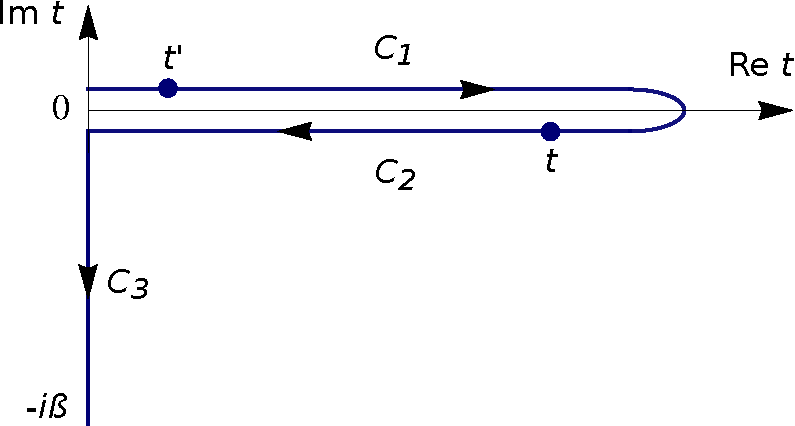
\includegraphics[width=0.5\linewidth]{Chapters/Theory_Kelgysh/figure/kadanoff-baym_contour.pdf}} 
\caption{L-shaped contour}
\label{L-shaped contour}
\end{figure}

	
Finally, the time-dependent expectation value with respect of initial equilibrium and the time-dependent density matrix can be expressed as
\begin{align}
\left\langle O(t) \right\rangle =\dfrac{1}{Z}
Tr\left[ U(-i \beta,0) U(0,t) O U(t,0) \right] =
\dfrac{Tr\left[ T_C e^{-i \int_C d \hat{t} H(\hat{t}) O(t) } \right] }{Tr\left[ T_C e^{-i \int_C d \hat{t} H(\hat{t})} \right] }
\label{expectation value2}
\end{align}
where $T_{C}$ is a contour-ordering operator that organize operators on the contour $C$ in the order 
 $0 \rightarrow t_{max} \rightarrow 0 \rightarrow -i \beta$ (Fig.~\ref{L-shaped contour}), $O(t)$ indicates that the operator $O$ is inserted at time $t$ on the contour $C$ \citep{bookKadanoff_and_Baym}.
 
Such time parametrization along the contour allows us to derive many techniques from equilibrium many-body theory to nonequilibrium. 
It should be noted that other time contours can also be used depending on the physical situation.


	
\FloatBarrier
\subsection{Contur-ordered Green's functions and self-energy}
	
One particle contour-ordering Green's functions is defined according to
\begin{align}
G(t,t')
&\equiv
-i\langle T_{C}\, c(t)\, c^\dagger(t')\rangle,
\label{green def}
\end{align}

where $c^{\dagger}$($c$) is a creation (annihilation) operator of particles, and $t,t' \in C$. Spin and orbital indices are not shown to simplify writing equations.

The contour $C$ is divided into three branches $C_1$, $C_2$ and $C_3$ as in Fig.~\ref{L-shaped contour}. there are nine possibilities to distribute the arguments along the contour, which can be grouped in a $(3 \times 3)$ matrix \citep{PhysRevB.44.6104}. 

Each component of the Green's functions satisfies
\begin{subequations}
\begin{align}
 \label{redundancy-1}
 G^{11}(t,t')
  &=
   G^{12}(t,t') \quad ({\rm for}\; t\le t'),
 \\
 G^{11}(t,t')
  &=
   G^{21}(t,t') \quad ({\rm for}\; t>t'),
 \\
 G^{22}(t,t')
  &=
   G^{21}(t,t') \quad ({\rm for}\; t<t'),
 \\
 \label{redundancy-4}
 G^{22}(t,t')
  &=
   G^{12}(t,t') \quad ({\rm for}\; t\ge t'),
 \\
 G^{13}(t,\tau ')
  &=
   G^{23}(t,\tau '),
 \\
 G^{31}(\tau,t')
  &=
   G^{32}(\tau,t').
\end{align}
\label{redundancy}
\end{subequations}


Some components can be summarized as
\begin{align}
G^{11}(t,t')+G^{22}(t,t')
 &=
  G^{12}(t,t')+G^{21}(t,t'). 
\label{linear dependence1}
\end{align}

But such matrix representation is overcomplete because not all components are independent. One can reduce $(3 \times 3)$ matrix using linear transformation (Keldysh rotation),
\begin{align}
 \hat{G}
  &=
   \begin{pmatrix}
    G^{R} & G^{K} & \sqrt{2} G^{\lh} \\
    0 & G^{A} & 0 \\
    0 & \sqrt{2} G^{\rh} & G^{M}
   \end{pmatrix}
   =L\tau_3
   \begin{pmatrix}
    G^{11}(t,t') & G^{12}(t,t') & G^{13}(t,\tau ') \\
    G^{21}(t,t') & G^{22}(t,t') & G^{23}(t,\tau ') \\
    G^{31}(\tau,t') & G^{32}(\tau,t') & G^{33}(\tau,\tau')
   \end{pmatrix}L^{\dagger}.
 \label{G_3x3}
\end{align}
where rotating $L$ and Pauli $\tau_3$ matrices,
\begin{align}
 L
  &=\frac{1}{\sqrt{2}}
   \begin{pmatrix}
    1 & -1 & 0 \\
    1 & 1 & 0 \\
    0 & 0 & \sqrt{2}
   \end{pmatrix}
    , \: \: \: \: \tau_3=
   \begin{pmatrix}
    1 & 0 & 0 \\
    0 & -1 & 0 \\
    0 & 0 & 1
   \end{pmatrix}.
 \label{rotating_pauli}
\end{align}

Thus, only six linearly independent Greens functions remain. They are called as retarded ($G^R$), advanced ($G^A$), Keldysh ($G^K$), left-mixing ($G^{\lh}$), right-mixing ($G^{\rh}$), and Matsubara Green's function ($G^M$). They can be parameterized as follows
\begin{subequations}
\label{physical green def}
\begin{align}
G^R(t,t')
 &=
   \tfrac12(G^{11}(t,t')-G^{12}(t,t')+G^{21}(t,t')-G^{22}(t,t'))
\nonumber
\\
 &=
  -i\theta(t-t') \langle [c(t),c^\dagger(t')]_\mp \rangle,
\\
G^A(t,t')
 &=
   \tfrac12(G^{11}(t,t')+G^{12}(t,t')-G^{21}(t,t')-G^{22}(t,t'))
\nonumber
\\
 &=
  i\theta(t'-t) \langle [c(t),c^\dagger(t')]_\mp \rangle,
\label{advanced green def}
\\
G^K(t,t')
 &=
   \tfrac12(G^{11}(t,t')+G^{12}(t,t')+G^{21}(t,t')+G^{22}(t,t'))
\nonumber
\\
 &=
  -i \langle [c(t),c^\dagger(t')]_\pm \rangle,
\label{keldysh green function}
\\
G^{\lh}(t,\tau ')
 &=
   \tfrac12(G^{13}(t,\tau ')+G^{23}(t,\tau '))
 =
   \mp i \langle c^\dagger(\tau ') c(t) \rangle,
\\
G^{\rh}(\tau, t')
 &=
   \tfrac12(G^{31}(\tau,t')+G^{32}(\tau,t'))
 =
   -i\langle c(\tau) c^\dagger(t') \rangle,
\\ \:
\:G^M(\tau,\tau ')
 &=
   -iG^{33}(\tau,\tau')
 =
   -\langle \mathcal{T}_\tau\, c(\tau) c^\dagger(\tau ') \rangle.  
\end{align}
\end{subequations}

Correlation functions $G^{>}$ and $G^{<}$ which correspond propagation of a "particle" and a "hole":
\begin{align}
\label{gles def}
 G^<(t,t')
  &=
   G^{12}(t,t')
  =
   \mp i \langle c^\dagger(t') c(t) \rangle
  = \tfrac12
   (G^K(t,t')-G^R(t,t')+G^A(t,t')),  
 \\
\label{ggtr def}
 G^>(t,t')
  &=
   G^{21}(t,t')
  =
   -i \langle c(t) c^\dagger(t') \rangle
  = \tfrac12
   (G^K(t,t')+G^R(t,t')-G^A(t,t')).
\end{align}

Using the above contur-ordered Green's function one can rewrite as inverse adopting for noninteracting tight-binding Hamiltonian $H_0(t)=\sum_k[\epsilon_k(t)-\mu]c_k^\dagger c_k$:
\begin{align}
\label{G0inv_k}
G^{-1}_{0,k}(t,t')=[i\partial_t+\mu -\varepsilon_k(t)]\delta_C(t,t')
\end{align}
where $\delta_C(t,t')=\partial_t \theta_C(t,t')$.

It is possible to describe the many-body interactions of a single particle by introducing an energy dependent effective potential called self-energy ($\Sigma$). Similar to the Green's functions the self-energy is defined on the L-shaped contour and has a $(3 \times 3)$ matrix structure which can be reduced using the Keldysh rotation \citep{PhysRevB.44.6104}:
\begin{align}
 \hat{\Sigma}
  &=
   \begin{pmatrix}
    \Sigma^{R} & \Sigma^{K} & \sqrt{2} \Sigma^{\lh} \\
    0 & \Sigma^{A} & 0 \\
    0 & \sqrt{2} \Sigma^{\rh} & \Sigma^{M}
   \end{pmatrix}
   =L\tau_3
   \begin{pmatrix}
    \Sigma^{11}(t,t') & \Sigma^{12}(t,t') & \Sigma^{13}(t,\tau ') \\
    \Sigma^{21}(t,t') & \Sigma^{22}(t,t') & \Sigma^{23}(t,\tau ') \\
    \Sigma^{31}(\tau,t') & \Sigma^{32}(\tau,t') & \Sigma^{33}(\tau,\tau')
   \end{pmatrix}L^{\dagger}.
 \label{S 3x3}
\end{align}
These components are called as retarded ($\Sigma^R$), advanced ($\Sigma^A$), Keldysh ($\Sigma^K$), left-mixing ($\Sigma^{\lh}$), right-mixing ($\Sigma^{\rh}$), and Matsubara ($\Sigma^M$).

The self-energy operator is related to the bare $G_0$ and dressed $G$ propagators and via the Dyson equation: 
\begin{align}
\label{dyson1}
\hat{G} = \hat{G_0} + \hat{G_0} \convz \hat{\Sigma} \convz \hat{G}.
\end{align}
where $*$ denotes convolution. Using a differential form for $G_0^{-1}$ this expression can be rewritten for various components as
\begin{align}
\label{dyson2}
&[i\partial_t - \mu +\varepsilon_k(t) ] G(t,t') - \int_\CC \!d\bar t\, \Sigma(t,\bar t) G(\bar t,t') 
= \delta_\CC(t,t')
\end{align}
From the physical point of view, the solutions of this equation describe the time-dependent single-particle spectrum $(G^R)$ and particle distribution $(G^<)$.


\FloatBarrier

\section{Hubbard model}
\label{section:Hubbard_model}
In 1960s the Hubbard model was proposed by Hubbard \citep{doi:10.1098/rspa.1963.0204}, Gutzwiller \citep{PhysRevLett.10.159} and Kanamori \citep{1963PThPh..30..275K} to describe electrons in $3d$ transition metal monoxides (FeO, NiO, CoO). 

The Hubbard model is one of the most important models in theoretical physics due to its simplicity and the number of physical phenomena that it can describe. These phenomena include metal-insulator transition, antiferromagnetism, ferrimagnetism, ferromagnetism, and superconductivity. 
Hamiltonian for single-band Hubbard model with time-dependent hopping amplitudes and local Coulomb repulsion,
\begin{subequations}
\begin{align}
\label{Habbard_Hamiltonian}
&
H(t)=H_{kin}(t)+H_{pot}(t)
\\
\label{Habbard_Hamiltonian_kin}
&
H_{kin}(t)=\sum_{ij\sigma} {t_{ij}(t)c^{\dagger}_{i \sigma} c_{j \sigma}}
\\
\label{Habbard_Hamiltonian_pot}
&
H_{pot}(t)=U(t) \sum_i{(n_{i\uparrow}-\frac{1}{2})(n_{i\downarrow}-\frac{1}{2})}
\end{align}
\end{subequations}
where $c^{\dagger}_{i \sigma}(c_{j \sigma})$ are creation (annihilation) operators for an electron with the spin $\sigma$ in the orbital at the lattice site $i$, $n_{i\sigma}=c^{\dagger}_{i \sigma} c_{j \sigma}$ counts the number of electrons with the spin $\sigma$ in the orbital at site $i$. The kinetic energy $H_{kin}(t)$ allows for tunneling of particles between sites of the lattice with amplitudes $t_{ij}(t)$. Potential term of the Hamiltonian $H_{pot}(t)$ corresponds of an on-site Coulomb interaction.

Due to recent growth of experimental interest in the systems driven out of equilibrium, such as the ultrafast pump-probe spectroscopies, theoretical methods to study such correlated systems are necessary. Thus, in later chapters, we will investigate the behavior of the Hubbard model out of equilibrium under the action of an external electromagnetic field. To do this, we describe the external spatially uniform electric field via the vector potential ${\bf A}(t)$
\begin{align}
\label{Vector_potential}
{\bf E(t)} = -\partial{\bf A}(t)/\partial t
\end{align}

The Peierls substitution \citep{Peierls1933} is used to account for the electric field in the Hamiltonian, so the hopping matrix in the general case elements satisfy
\begin{align}
\label{hoppings_1}
t_{ij}(t)=t_{ij}exp \left(-\int_{{\bf R}_i}^{{\bf R}_j} d{\bf r} {\bf A}({\bf{r}},t)\right)  
\end{align}

For the tight-binding parametrization of the electronic structure of the $CuO$ plane, which is a common feature of high-$T_c$ superconducting materials, we use the following dispersion law for a square lattice in the $k$-space:
\begin{subequations}
\begin{align}
\label{dispersion_1}
\varepsilon_1(k,t)
&=
{2t_1(cos(k_x+ A_x(t))+cos(k_y+A_y(t)))},
\\
\label{dispersion_2}
\varepsilon_2(k,t)
&=
	2t_1(cos(k_x+A_x(t))+cos(k_y+A_y(t)))
		\nonumber
		\\
 &+
4t_2(cos(k_x+A_x(t))\cdot cos(k_y+A_y(t))).
\end{align}
\end{subequations}
where $\varepsilon_1(k,t)$ corresponds to nearest neighbor (NN) approximation and $\varepsilon_2(k,t)$ next nearest neighbor (NNN).

Due to the fact that DMFT becomes exact in the limit of lattices with an infinite coordination we use for benchmarks the Bethe lattice with semielliptic density of states:
\begin{align}
\label{Bethe_lattice}
\rho(\varepsilon)=\dfrac{2\sqrt{1-(\varepsilon/D)^2}}{\pi D}
\end{align}
where $D$ is half-bandwidth.

The model has two extreme cases: 1) Limit with $U\rightarrow 0$ is a tight-binding model which entirely analogous for the investigation of spinless free fermions; 2) Limit with $t\rightarrow 0$ is called atomic limit where the electrons can not move, such case represent the Mott insulator.

\FloatBarrier

\section{ Nonequilibrium dynamical mean-field theory}
\label{section:NE_DMFT}
In equilibrium, the DMFT \citep{RevModPhys.68.13} plays a large role in understanding systems with strong electron correlations. An example of such DMFT success is explanation transition between a metal and the Mott insulator, and in combination with other theories for realistic simulation of many correlated materials. 

This chapter presents the nonequilibrium dynamical mean-field theory (NE-DMFT) \citep{RevModPhys.86.779} which allows studying the strongly correlated many-body systems out of equilibrium. 


\FloatBarrier
\subsection{Self-consistency loop}
An approximation of equilibrium and out of equilibrium DMFT is the local nature of the self-energy. This means that self-energy is momentum-independent.
\begin{equation}
\Sigma_{ij}^\text{lat}(t,t')\approx \delta_{ij}\Sigma^\text{imp}(t,t').
\end{equation}
This fact allows mapping of a lattice problem to a self-consistent solution of a quantum impurity model, which is exact in the limit of infinite dimensions. 
We can write nonequilibrium single-site action as
\begin{align}
\label{Action}
S_{imp}=-i\int_C dt H_{pot}(t)-i\sum_{\sigma}{\int_C dt dt' c^{\dagger}_{\sigma}(t) \Delta_i (t,t') c_{\sigma}(t')}
\end{align}
where $\Delta_i (t,t')$ is time-dependent hybridization function wich represents the hopping amplitude from the impurity into the bath \citep{PhysRevB.45.6479}.

After that we can define the contour-ordered impurity Green’s function
\begin{align}
\label{Green_imp}
G_{imp}(t,t')=-i\langle T_C c(t) c^{\dagger}(t') \rangle_{S_{imp}}
\end{align}
where $\langle...\rangle_{S_{imp}}=\dfrac{Tr\left[T_C exp (S_{imp})\cdots\right] }{Tr \left[T_C exp (S_{imp})\right]}$ the expectation value of observables.

The time-dependent Weiss Green's function is the Green's function of non-interacting impurity and related with the hybridization function:
\begin{align}
\label{Green_Weiss}
\mathcal{G}(t,t')=(i\partial_t+\mu(t))\delta_C(t,t')-\Delta(t,t')
\end{align}

The lattice and Weiss Green's functions need to be determined iteratively.

 
1) This self-consistent loop starts with the calculation of the impurity Green's function $G_{imp}(t,t')$ and $\mathcal{G}(t,t')$.

2) From impurity Green's function the self-energy can be extracted using the Dyson's equation: $\Sigma_{imp}(t,t')=\mathcal{G}^{-1}(t,t')-G_{imp}^{-1}(t,t')$

3) Due to DMFT approximation, identify the lattice self-energy with the impurity one, $\Sigma_{\bf k}(t,t')=\Sigma_{imp}(t,t')$. The local lattice Green’s function by integrating over all ${\bf k}$-points in the first Brilluin zone $G_{loc}(t,t')=\int(d {\bf k})[(i\partial_t+\mu(t)-\varepsilon_{\bf k}(t))\delta_C(t,t')-\Sigma_{imp}(t,t')]^{-1}$

4) The self-consistency condition of the DMFT is $G_{loc}(t,t')=G_{imp}(t,t')$. Use this definition to define a new Weiss Green's function $\mathcal{G}^{-1}(t,t')=G_{loc}^{-1}(t,t')+\Sigma_{imp}(t,t')$. To enhance the convergence of the self-consistency loop one can mixed new and old Weiss field: $\mathcal{G}_{new}^{-1}(t,t')=(1-\xi)\mathcal{G}_{old}^{-1}(t,t')+\xi \left[G_{loc}^{-1}(t,t') + \Sigma_{imp}(t,t') \right]$.


\FloatBarrier
\subsection{Equal-time observables}
The lattice Green's functions which we obtain after the NEDMFT iterations allows us compute physical observables:

Using definition of lesser Green function expression for the number of particles with spin $\sigma$ on site $i$ written as:
\begin{align}
\label{Number_of_particles}
n_{\sigma}(t)=\dfrac{1}{L}\sum_i {\left\langle c_{i \sigma}^{\dagger}(t) c_{i \sigma}(t)\right\rangle} = -iG_{\sigma}^{<}(t,t),
\end{align}
here $L$ is the lattice site.

A momentum ocupation we obtain from the ${\bf k}$-resolved Green's function
\begin{align}
\label{Number_of_particles_k}
n({\bf \tilde{k}},t)=-iG_{{\bf k}+{\bf A}(t),\sigma}^{<}(t,t)=-i\tilde{G}_{{\bf k},\sigma}^{<}(t,t)
\end{align}
this is the gage invariant form, where wave vector is ${\bf \tilde{k}}={\bf k}+{\bf A}(t)$ \citep{PhysRevB.38.1667}.

The current operator \citep{PhysRevLett.68.2830} is defined as
\begin{align}
\label{Current}
{\bf j}(t)
&
=\dfrac{e}{V}\sum_{{\bf k} \sigma} v_{\bf k}(t)n_{\tilde{\bf k}, \sigma}(t)
\\
&
=-\dfrac{ie}{V}\sum_{{\bf k} \sigma} v_{{\bf k}-{\bf A}(t)} G_{{\bf k},\sigma}^{<}(t,t) =-\dfrac{ie}{V}\sum_{{\bf k} \sigma} v_{\bf k} G_{{\bf k}+{\bf A}(t),\sigma}^{<}(t,t)=-\dfrac{ie}{V}\sum_{{\bf k} \sigma} v_{\bf k} \tilde{G}_{{\bf k},\sigma}^{<}(t,t),
\end{align}
where $V$ is the volume, $v_k$ - group velocity (derivative of the dispersion law).


The kinetic energy per lattice site 
\begin{align}
\label{Kinetic_energy}
E_{kin}(t)=\dfrac{1}{L}\sum_{{\bf k} \sigma} \varepsilon_{{\bf k}, \sigma}{\left\langle c_{{\bf k} \sigma}^{\dagger}(t) c_{{\bf k} \sigma}(t)\right\rangle}
=-\dfrac{i}{L} \sum_{{\bf k} \sigma} \varepsilon_{{\bf k}, \sigma}G_{{\bf k},\sigma}^{<}(t,t).
\end{align}

The double occupation per lattice site
\begin{align}
\label{Double_occupation}
d(t)=\dfrac{1}{L}\sum_i{ \left\langle {n}_{i\uparrow}(t) {n}_{i\downarrow}(t) \right\rangle }.
\end{align}

The interaction energy
\begin{align}
\label{Interaction_energy}
E_{pot}(t)
&
=U(t) \sum_{i}\left\langle 
\left( {n}_{i\uparrow}(t)-\dfrac{1}{2} \right) 
\left( {n}_{i\downarrow}(t)-\dfrac{1}{2} \right) \right\rangle
\\ 
&
= U(t)\left[ d(t)-\dfrac{1}{2} \left({n}_{\uparrow}(t) + {n}_{\downarrow}(t) \right) +\dfrac{1}{4} \right]. 
\end{align}

The total energy is a sum of the kinetic and potential energies:
\begin{align}
\label{Total_energy}
E_{tot}(t)=E_{kin}(t)+E_{pot}(t).
\end{align}

\FloatBarrier
\subsection{Spectral function and photoemission spectrum}
\label{subsection:Spectral_function}
A pump-probe time-resolved photoemission spectroscopy (TRPES) [see Sec. \ref{PP_s}] and a angular-resolved photoemission spectroscopy(TRARPES) allows to probe the excited state non-equilibrium dynamics of electrons in solids. These methods can provide data about time-dependent electronic structure of strongly correlated materials.

DMFT based retarded and lesser Green's functions can give information about the excitation and occupation spectrum \citep{PhysRevB.81.115131}, which is closely related with the intensity in TRPES:
\begin{align}
\label{Spectr_R_L_1}
&
A^R(t,\omega)=-\dfrac{1}{\pi}Im \int_0^t ds e^{i\omega s}G^R(t,t-s),
\\
&
A^<(t,\omega)=\dfrac{1}{\pi}Im \int_0^t ds e^{i\omega s}G^<(t,t-s).
\label{Spectr_R_L_2}
\end{align}

The $k$-resolved spectral function and occupied density of states which is associated with TRARPES are calculated by the formulas:
\begin{align}
\label{Spectr_R_L_k_1}
&
A^R(t,\omega)_k=-\dfrac{1}{\pi}Im \int_0^t ds e^{i\omega s}G^R_k(t,t-s),
\\
&
A^<(t,\omega)_k=\dfrac{1}{\pi}Im \int_0^t ds e^{i\omega s}G^<_k(t,t-s).
\label{Spectr_R_L_k_2}
\end{align}

The photoemission intensity of emitted electrons under action of a short probe pulse as a function of energy and time-delay \citep{PhysRevB.95.115132}:
\begin{align}
\label{PES}
I(\omega,t_p)=-i\int dtdt'S(t)S(t')e^{i\omega(t-t')}G^{<}(t+t_p,t'+t_p)
\end{align}
here $t_p$ is time-delay between the pump and probe pulses; $S(t)$ - probe envelope. 
These TRPES equations has frequancy-time uncertainty. If the probe pulse is very short one measures the occupation density using Wigner transorm of the lesser Green's function $I(\omega,t_p)=\int ds e^{i\omega t_p} G^< (t_p+s/2,t_p-s/2)$, but lost good energy resolution.
It is also important to note such an expression of the photoemission spectrum neglects interactions between the outgoing electron and the bulk (sudden approximation).


\FloatBarrier
\subsection{Impurity solvers}
\label{subsection:Impurity_solvers}
As we discussed earlier, the lattice model of correlated electrons is mapped onto the Anderson impurity model (AIM) by neglecting the nonlocal electron correlations.

To solve the impurity problem in time-dependent systems numerically is much expensive compared to equilibrium as one must manipulate the contour-ordered objects such as Green's function and self-energy that depends on two-time variables. 

The most popular exact time-dependent impurity solvers:

1) Continuous-time quantum Monte Carlo (CT-QMC)\citep{RevModPhys.83.349,PhysRevLett.100.176403,PhysRevB.79.035320,PhysRevLett.106.236401}. There are several varieties of this solver, interaction expansion (CT-INT)\citep{PhysRevB.81.035108,PhysRevB.72.035122,Gull_2008,PhysRevB.79.035320} and hybridisation expansion (CT-HYB)\citep{PhysRevLett.100.176403,PhysRevB.79.153302,PhysRevB.79.035320}. The disadvantage of these methods is the high cost of calculations in which the computation time grows exponentially with simulation time. There is the successful extension of CT-HYB is Inchworm QMC\citep{PhysRevLett.115.266802,PhysRevB.95.085144,PhysRevB.96.155126}, where the computational time grows polynomially.

2) Density matrix renormalization group (DMRG)\citep{RevModPhys.77.259, PhysRevB.95.165139, PhysRevLett.93.040502, PhysRevLett.93.076401}. Here the computation time also grows exponentially with modeling time.

3) Exact diagonalization (ED)\citep{PhysRevB.88.235106,PhysRevB.91.045136}. In this method, the simulation time may be large, but there is a limit of lattice sites.

As well there are many approximate impurity solvers:

1) Iterated perturbation theory (IPT)\citep{PhysRevLett.107.186406, PhysRevB.81.115131,PhysRevB.88.165115, PhysRevB.91.245153}. Approximation based on second-order perturbation theory in terms of Coulomb interaction. It works well in a weak-coupling regime and was found that accidentally reproduce the strong-coupling limit and is believed to describe moderate and strong-coupling regimes qualitatively.

2) Noncrossing approximation (NCA)\citep{PhysRevB.49.11040, PhysRevB.82.115115} and 
one-crossing approximation (OCA)\citep{PhysRevB.92.195123, PhysRevB.99.045118}. They are conserving approximations and based on strong-coupling perturbation theory. In this way, one can treat strongly interacting systems.

In nonequilibrium physics, it is essential to have sufficient simulation time for presentation observables properties and to understand ultrafast processes. Therefore, in this thesis, we developed and used some perturbation methods based on weak coupling expansion, which requires reasonable computational time. 

Thus we calculate the momentum independent self-energies for weak coupling expansion \citep{1989AnPhy.193..206B}:

{Hartree-Fock self-energy}:
\begin{align}
\label{HF_single_band}
\Sigma^{HF}(t)=U(t)n(t)
\end{align}

{Second order self-energy}:
\begin{align}
\label{S2_single_band}
\Sigma^{2}(t,t')=i V^2(t,t')G(t,t') 
\end{align}
where potential given by
\begin{align}
\label{V2_single_band}
V^2(t,t')=U(t)\chi^{PH}_0(t,t')U(t')
\end{align}
here bare particle-hole polarization bubble:
\begin{align}
\label{chi02_single_band}
\chi^{PH}_0(t,t')=-iG(t,t')G(t',t)
\end{align}

{Self-energy for particle-hole channel}:
\begin{align}
\label{Sph_single_band}
\Sigma^{PH}(t,t')=iV^{PH}(t,t')G(t,t')
\end{align}
where potential of the particle-hole channel has charge and magnetic contributions:

\begin{align}
\label{Vph_single_band}
V^{PH}(t,t')
&=\dfrac{1}{2}\left[ U_d(t) \left( \chi_d^{PH}(t,t')-\chi_{0d}^{PH}(t,t') \right) U_d(t') \right] 
\nonumber
		\\
&+ \dfrac{3}{2} \left[ U_m(t) \left( \chi_m^{PH}(t,t')-\chi_{0m}^{PH}(t,t') \right) U_m(t') \right]
\end{align}


The total propagators of charge and magnetic parts of the channel have to be found from RPA-like equation:
\begin{align}
\label{chiph_d_single_band}
\chi^{PH}_d(t,t')=\chi^{PH}_{0d}(t,t')+\int_C \chi^{PH}_{0d}(t,t_1) U_d(t_1) \chi^{PH}_d(t_1,t') dt_1
\end{align}
\begin{align}
\label{chiph_m_single_band}
\chi^{PH}_m(t,t')=\chi^{PH}_{0m}(t,t')+\int_C \chi^{PH}_{0m}(t,t_1) U_m(t_1) \chi^{PH}_m(t_1,t') dt_1
\end{align}
bare particle-hole polarization bubbles:
\begin{align}
\label{chiph_0_single_band}
\chi^{PH}_{0d}(t,t')=\chi^{PH}_{0m}(t,t')=-iG(t,t')G(t',t)
\end{align}

{Self-energy for particle-particle channel}:
\begin{align}
\label{Spp_single_band}
\Sigma^{PP}(t,t')=-iV^{PP}(t,t')G(t',t)
\end{align}
where a particle-particle potential is given by
\begin{align}
\label{Vpp_single_band}
V^{PP}(t,t')= U_s(t) \left( \chi_s^{PP}(t,t')-\chi_{0s}^{PP}(t,t') \right) U_s(t') 
\end{align}
The total propagator has to be found as:
\begin{align}
\label{chipp_s_single_band}
\chi^{PP}_s(t,t')=\chi^{PP}_{0s}(t,t')+\int_C \chi^{PP}_{0s}(t,t_1) U_s(t_1) \chi^{PP}_s(t_1,t') dt_1
\end{align}
bare particle-particle polarization bubbles:
\begin{align}
\label{chipp_0_single_band}
\chi^{PP}_{0s}(t,t')=iG(t,t')G(t,t').
\end{align}
The Coulomb interaction for different channels is renormalized as
$U_d(t)=U(t)$, $U_m(t)=-U(t)$, $U_s(t)=U(t)$.

Thus the second order self-energy (SOPT):
\begin{align}
\label{S_so_single_band}
\Sigma^{SOPT}(t,t')=\Sigma^{HF}(t)+\Sigma^{2}(t,t').
\end{align}

The self-energy for the particle-hole T-matrix approximation (TMA-PH):
% is sums the series of particle-hole ladder diagrams:
\begin{align}
\label{Stma_ph_single_band}
\Sigma^{TMA-PH}(t,t')=\Sigma^{HF}(t)+\Sigma^{2}(t,t')+\Sigma^{PH}(t,t').
\end{align}

The self-energy for the particle-particle T-matrix approximation (TMA-PP):
% is sums the series of particle-particle ladder diagrams:
\begin{align}
\label{Stma_pp_single_band}
\Sigma^{TMA-PP}(t,t')=\Sigma^{HF}(t)+\Sigma^{2}(t,t')+\Sigma^{PP}(t,t').
\end{align}

The self-energy for the fluctuation-exchange approximation (FLEX):
% bubble, particle-particle, and particle-hole ladder diagrams are included:
\begin{align}
\label{Sflex_single_band}
\Sigma^{FLEX}(t,t')=\Sigma^{HF}(t)+\Sigma^{2}(t,t')+\Sigma^{PH}(t,t')+\Sigma^{PP}(t,t').
\end{align}

Below we provide calculations for the 2D square lattice Eq. \eqref{dispersion_1}, hopping amplitude $t=1$, inverse temperature $\beta=1/T=10$ and $64 \times 64$ $k$-grid. 

In Fig.~\ref{Eq_comp_DOS} two density of states representing DMFT+TMA-PH are calculated using different codes: red line analytic continuation from imaginary axis and blue line getting using the real-time Keldysh contour. Both results are fit well. 
\begin{figure}[h!]
\center{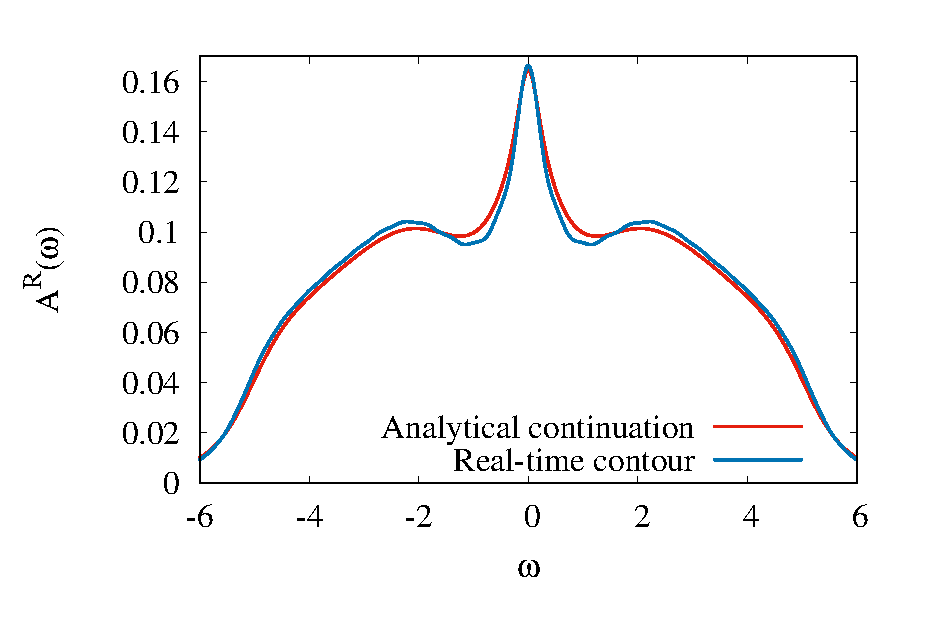
\includegraphics[width=0.5\linewidth]{Chapters/Theory_Kelgysh/figure/DOS_comp.eps}} 
\caption{Comparison of DMFT+TMA-PH spectral functions obtained using different methods ($U=2.88$)}
\label{Eq_comp_DOS}
\end{figure}

In \citep{PhysRevB.91.235114} systematic studies of the accuracy calculating the self-energy for the single-band model was found that in weak-coupling regime second order perturbation theory is more reliable than performing additional channals summations. It is also known that the magnetic part of the particle-hole channal has a divergence in the denominator, which does not allow us to use it in the standard form of the DMFT scheme for $U>0.3W$($W$-bandwidth). Based on these, further calculations for the single-band model in this work will be provide using 2D square lattice and IPT scheme. 
\begin{figure}[h!]
\begin{minipage}[h]{0.5\linewidth}
\center{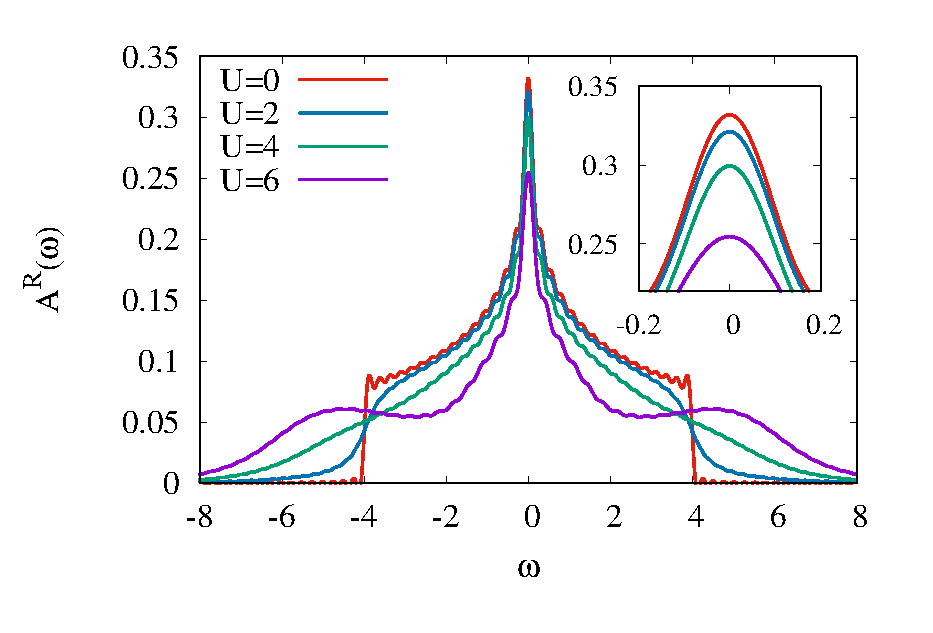
\includegraphics[width=1\linewidth]{Chapters/Theory_Kelgysh/figure/DOS_U.eps}} (a) \\
\end{minipage}
\hfill
\begin{minipage}[h]{0.5\linewidth}
\center{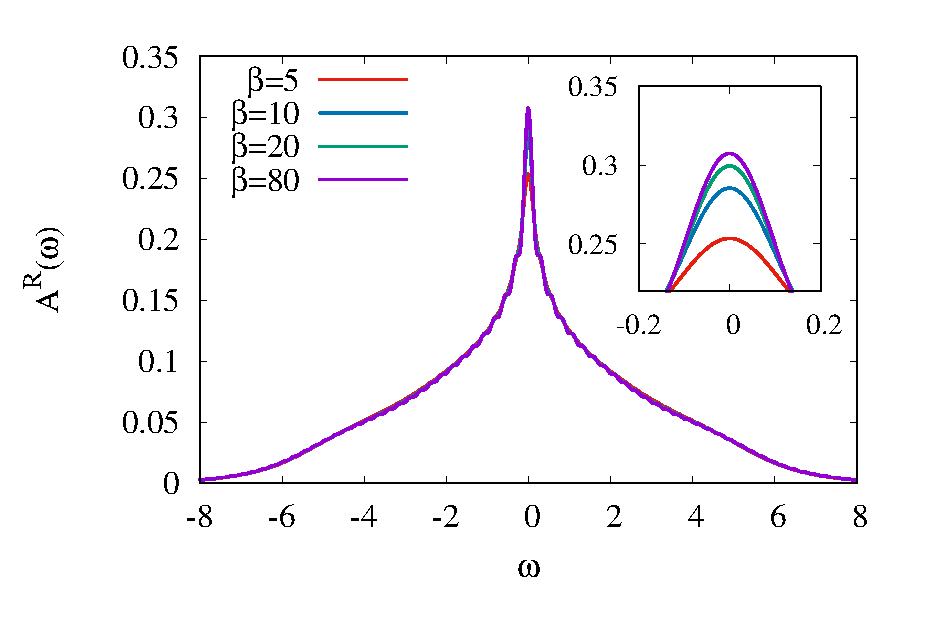
\includegraphics[width=1\linewidth]{Chapters/Theory_Kelgysh/figure/DOS_T.eps}} (b) \\
\end{minipage}
\caption{(a) IPT spectral function with different Coulomb interaction. (b) IPT spectral function with different inverse temperatures for $U=4$.}
\label{Eq_IPT_DOS}
\end{figure}

In Fig.~\ref{Eq_IPT_DOS}a equilibrium IPT spectral functions is characterized by different Coulomb interactions. Results for $U=0$ represent tight-binding model with $W=8$. With increasing interaction, we observe the disappearance of sharp edges and the gradual blurring of the density of states, which leads to an increase in the bandwidth. In a high $U=6$, the formation of three peak structures could be observed, which is present in the $U \sim W$ region. Decreasing temperature not significantly increase the peak height at $\omega=0$ (Fig.~\ref{Eq_IPT_DOS}b).

\FloatBarrier


\section{\label{PP_s}Appendix: Pump-probe spectroscopy}

Ultrafast time scale processes characteristic for a large number of physical phenomena, thereby induce great interest in fundamental and applied physics. The pump-probe spectroscopy \citep{Petek_Ogawa_1997,Axt_2004_Kuhn,ABRAMCZYK2005147} is the powerful and widely used experimental technique to study such nonequilibrium phenomena. Observation of fast processes is crucial to understanding ultrafast phase transitions, dynamics of various excitations, and many scattering processes.

%\citep{Zewail_Ahmed_2000,Petek_Ogawa_1997,Axt_2004_Kuhn}


%2) Схема эксперимента

\begin{figure}[h!]
\center{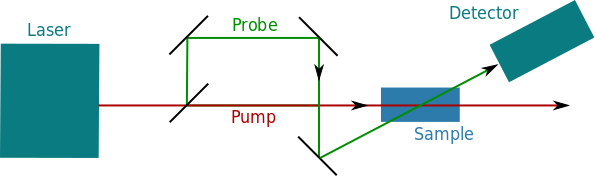
\includegraphics[width=0.6\linewidth]{Chapters/introduction_1/figure/PP_scheme.png}} \\
\caption{Schematic setup of the pump-probe spectroscopy.}
\label{fig:PES_scheme}
\end{figure}

In Fig.~\ref{fig:PES_scheme}, is shown a schematic picture of the pump-probe spectroscopy measurements. To study dynamical processes, the system must be perturbed from an equilibrium state to an excited one by using the "pump" beam. The excitement of the sample is possible with various parameters of the pump pulse including duration, intensity, polarization, and energy. Another higher frequency "probe" pulse is used to observe a transient response after the pump. Both pulses approach the sample on different paths determined by the arrangement of mirrors, which allow obtaining time-resolved data for physical quantities.

%3) Физика процесса
The distribution of photoelectrons in energy, angle and time gives information about the evolution of the electronic structure due to perturbation of the system. 
Access to nonequilibrium states of matter attainable through femtosecond IR \citep{C9CP00855A, PhysRevApplied.3.051002}, optical \citep{Steinmeyer1507, Hentschel_2001} or extreme ultraviolet lasers (EUV) and X-ray free
electron lasers \citep{McNeil_2010,Dunne_Mike_2018,Parra2003,Maltezopoulos_2008}.
At the moment, a large number of experiments and studies has been done for various materials: correlated insulators \citep{PhysRevLett.112.087402,PhysRevB.89.205114,PhysRevLett.113.216401}; graphene \citep{Nature_Materials_12_1119_1124,doi:10.1063/1.4871381} and graphitic materials \citep{PhysRevLett.76.483,PhysRevLett.87.267402,PhysRevLett.112.257401,PhysRevB.92.184303}; semiconductors \citep{RevModPhys.83.543,PhysRevB.81.113203}; cuprate superconductors \citep{PhysRevLett.99.197001,PhysRevLett.107.097002,Smallwood1137,Sci_Rep_6_18747_2016}; topological insulators \citep{Wang453,Sci_Rep_5_13213_2015,PhysRevLett.108.117403,PhysRevLett.109.127401,Nat_Commun_5_3003_2014,Sci_Rep_5_8160_2015,PhysRevLett.115.116801}; ultracold atoms \citep{PhysRevA.50.5025,PhysRevA.64.033421,PhysRevA.80.033404,}.




\chapter{Dynamical repulsive-to-attractive conversion of interactions}
\label{chap:pi_pulse}
\section{Introduction}
The creation of a population inversion in metallic bands corresponding to a negative temperature state \citep{PhysRev.81.279,PhysRev.103.20} is one of the ways to control the interparticle interaction. Such investigation was done in the work of \citep{PhysRevB.85.155124} for hypercubic lattice, where it was shown that it is possible to induce the population inversion in metallic systems using properly shaped half-cycle or monocycle pulses, the system without energy dissipation will thermalize in the negative temperature state after the pulse. Effective switching of the interaction from repulsive to attractive occurs because a density matrix $\exp ({-H/T})$ for a Hamiltonian $H$ with temperature $T < 0$ corresponds inverted $-H$ with $-T > 0$ \citep{PhysRevLett.105.220405,PhysRevLett.106.236401}.

In this chapter, we rely on the work \citep{PhysRevB.85.155124} taking realistic 2D square lattice and focused on transient nonequilibrium dynamics with different polarization of the electric field.
By the half-cycle pulse, we induce a shift in the momentum distribution of the electrons. Selecting the parameters of such pulse we can achieve half of the Brillouin zone, the system is brought to the negative-$T$ state, this is often (depending on the value of the interaction) leads to change of the interaction from repulsive to attractive.

Below we provide calculations for 2D square lattice with hopping amplitude $t=1$, initial inverse temperature $\beta=1/T=5$ and $32 \times 32$ $k$-grid. Time has units of reverse hoppings. 
%\clearpage
\section{Population invertion induced by a linear polarized pulse}

To investigate the effects of negative temperature state we use a single-band Hubbard model driven by the half-cycle electric field. The half-cycle pulses with amplitude of vector potential ($A_{max}$) and pulse length ($\tau$) chosen in $Y$ and $XY$ (diagonal) polarisation directions.
%The vector potential has the form:
%\begin{equation}
%A(t)=\frac{A_{max}}{\tau}(t-\tau sin(2\pi t/\tau))
%\end{equation}
%where $A_{max}$ - amplitude of vector potential; $\tau$ - pulse length.
\begin{figure}[h!]
\begin{minipage}[h]{0.5\linewidth}
\center{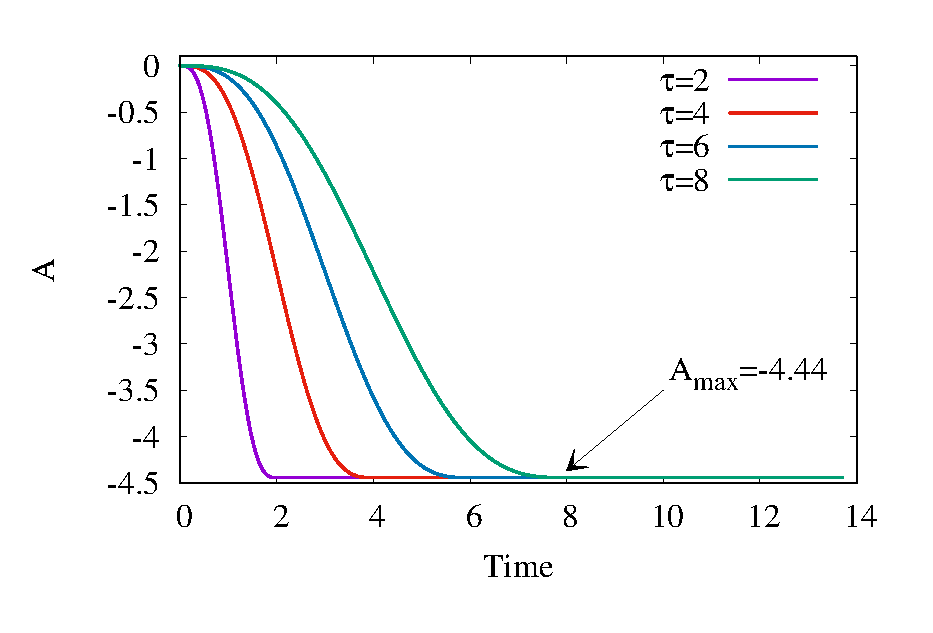
\includegraphics[width=1\linewidth]{Chapters/1_pi_pulse_tex/figure/xy/PulseA.eps}} (a) \\
\end{minipage}
\hfill
\begin{minipage}[h]{0.5\linewidth}
\center{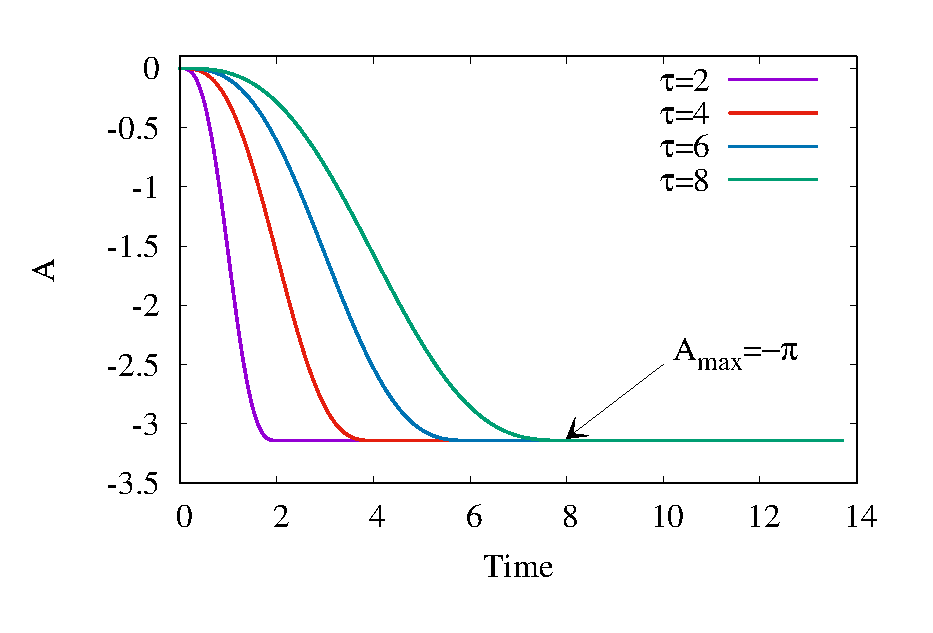
\includegraphics[width=1\linewidth]{Chapters/1_pi_pulse_tex/figure/y/PulseA.eps}} \\(b)
\end{minipage}
\begin{minipage}[h]{0.5\linewidth}
\center{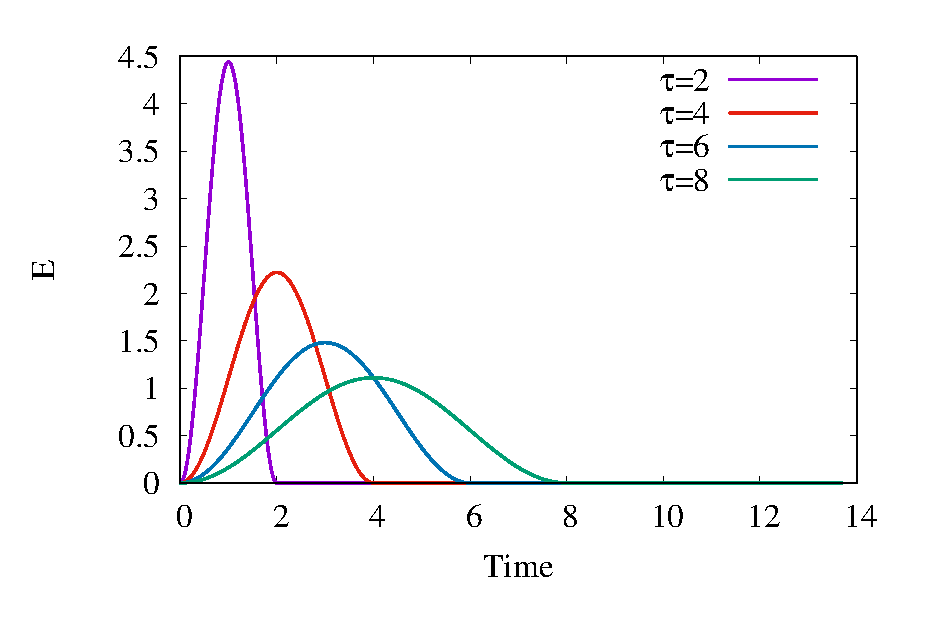
\includegraphics[width=1\linewidth]{Chapters/1_pi_pulse_tex/figure/xy/PulseE.eps}} (c) \\
\end{minipage}
\hfill
\begin{minipage}[h]{0.5\linewidth}
\center{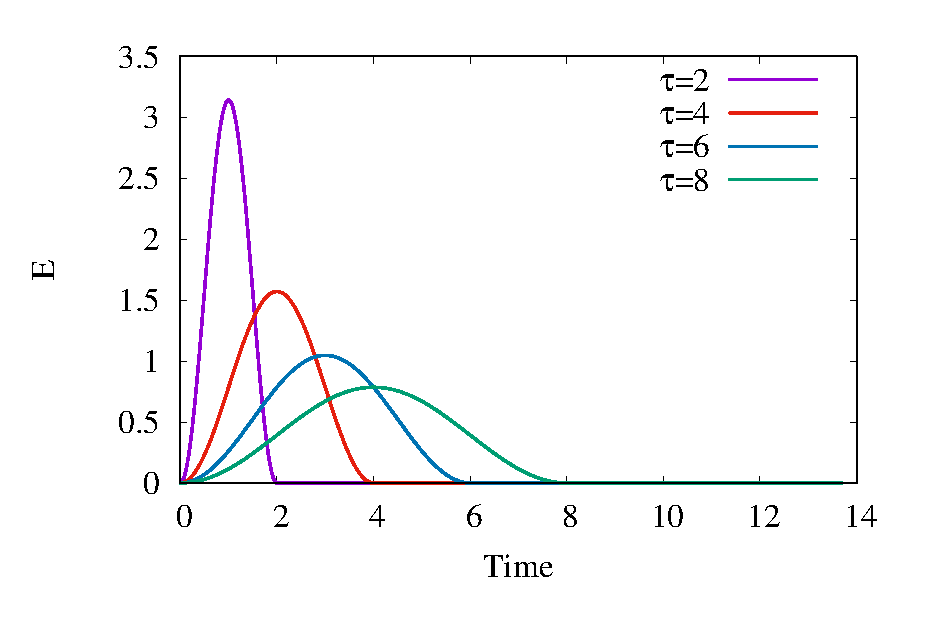
\includegraphics[width=1\linewidth]{Chapters/1_pi_pulse_tex/figure/y/PulseE.eps}} \\(d)
\end{minipage}
\caption{Vector potential and external electric field: (a),(c) for $XY$-polarization; (b),(d) for $Y$-polarization}
\label{fig:Pulses}
\end{figure}
In case of $Y$-polarization, the maximum value of the vector potential is as follows $A_{max} = \pi$ (Fig.~\ref{fig:Pulses}b). For diagonal polarization the maximum value of the vector potential $A_{max} =\pi*\sqrt{2}$ depicted in Fig.~\ref{fig:Pulses}a. The corresponding electric fields are shown in the Figs.~\ref{fig:Pulses}c,d. This allows to shift the momentum distribution in the case of $Y$-polarization from $\Gamma$ to Y, in the case of $XY$-polarization from $\Gamma$ to M in the Brillouin zone.

After the pulse excitation the isolated system strives to achieve a thermalized state with some effective temperature $T_{eff}$ and total energy $E_{tot}$. A thermal state with a positive temperature has $E_{tot} < 0$ at half filling, while $E_{tot} > 0$ happens at negative temperature ($T_{eff} < 0$). Thereby the total energy is an order parameter for the repulsion-to-attraction transition \citep{PhysRevB.85.155124}.

To show the effect of the population inversion we choose the half-cycle shape of the electric field with $\tau = 4$ (red line in Figs.~\ref{fig:Pulses}c,d) and investigate the behavior of the total energy and double occupancy (Fig.~\ref{fig:E_tot}).
\begin{figure}[h!]
\begin{minipage}[h]{0.5\linewidth}
\center{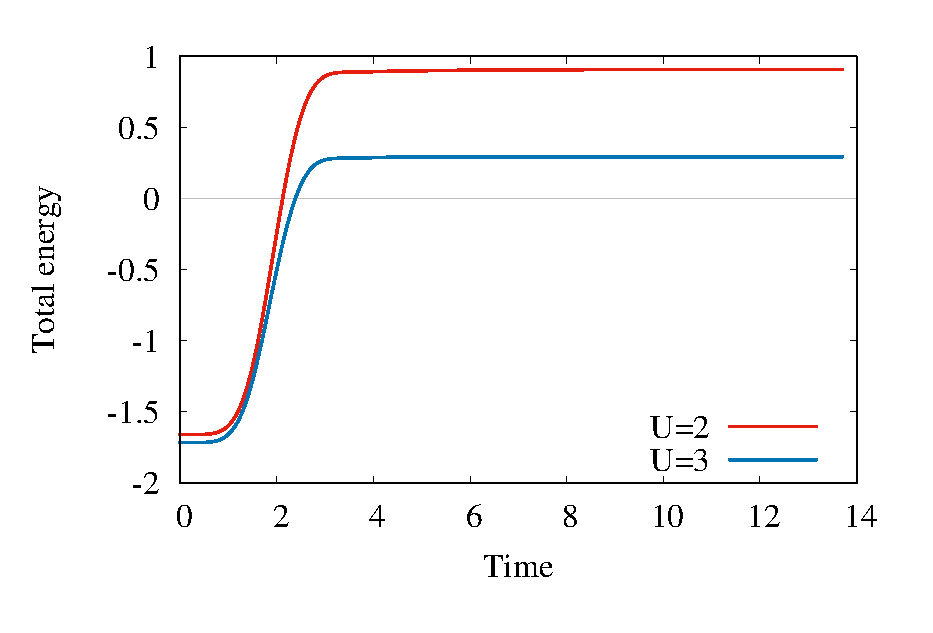
\includegraphics[width=1\linewidth]{Chapters/1_pi_pulse_tex/figure/xy/E_tot_xy.eps}} (a) \\
\end{minipage}
\hfill
\begin{minipage}[h]{0.5\linewidth}
\center{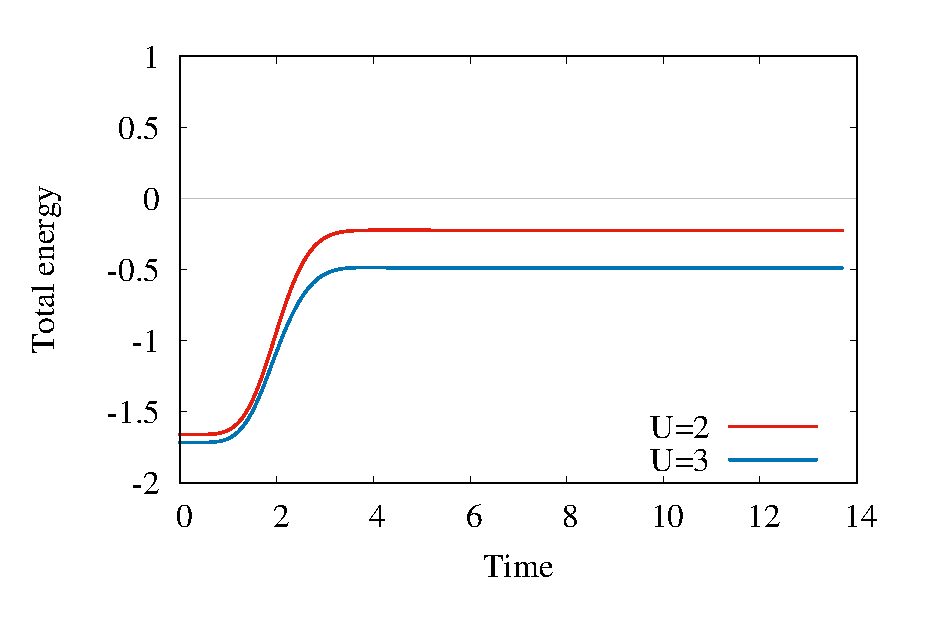
\includegraphics[width=1\linewidth]{Chapters/1_pi_pulse_tex/figure/y/E_tot_y.eps}} \\(b)
\end{minipage}
\begin{minipage}[h]{0.5\linewidth}
\center{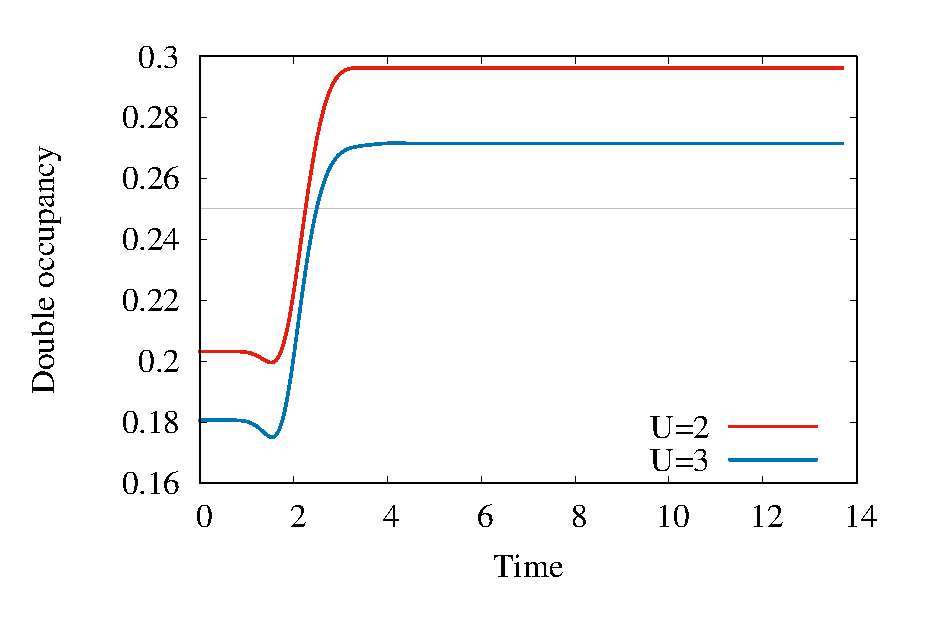
\includegraphics[width=1\linewidth]{Chapters/1_pi_pulse_tex/figure/xy/docc_xy.eps}} (c) \\
\end{minipage}
\hfill
\begin{minipage}[h]{0.5\linewidth}
\center{\includegraphics[width=1\linewidth]{Chapters/1_pi_pulse_tex/figure/y/docc_y.eps}} \\(d)
\end{minipage}
\caption{Total energy and double occupancy ($\tau = 4$): (a),(c) for $XY$ direction of pulse polarization ($A_{max} =\pi\sqrt{2}$); (b),(d) for $Y$-polarization ($A_{max} = \pi$).}
\label{fig:E_tot}
\end{figure}

From the analysis of Figs.~\ref{fig:E_tot}a,c we can observe a change in the sign of the interaction in case of field in the $XY$-polarization, $U=2$ and $U=3$. $E_{tot}>0$ (the total energy has the origin at zero) and the double occupancy $docc>0.25$ after the pulse. Then lower Coulomb interaction than $E_{tot}$ has a bigger value and a more pronounced effect of the negative temperature state after the pulse. In the case of $Y$-polarization of the electric field, the total energy negative all the time, so the interaction does not change the sign.
\begin{figure}[h!]
\center{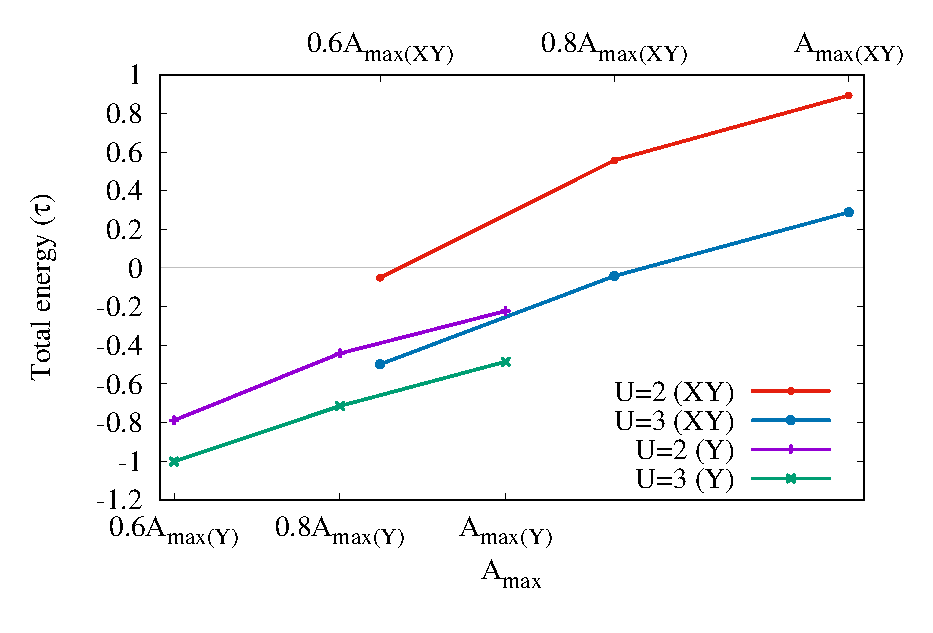
\includegraphics[width=0.7\linewidth]{Chapters/1_pi_pulse_tex/figure/xy/E_mpi.eps}} \\
\caption{The total energy after the pulse as a function of the magnitude of the vector potential ($\tau = 4$).}
\label{fig:E_tot_A}
\end{figure}

In the Fig.~\ref{fig:E_tot_A} is shown the total energy after the pulse for $\tau=4$ as a function of the magnitude of the vector potential for both polarizations. For the field in $XY$-polarization, there is positive total energy, which means that the sign of interaction has changed. The value of the total energy is maximum when the value of the amplitude of the vector potential such that exactly shift momentum distribution in the case of $Y$-polarization from $\Gamma$ to Y points in the Brillouin zone and the case of $XY$-polarization from $\Gamma$ to M. The value of the total energy decreases with increasing $U$. In the case of $Y$-polarization, there is no change in the sign of the interaction for all values of the vector potential and the Coulomb interaction. These statements are consistent with the results of the article \citep{PhysRevB.85.155124}.
\begin{figure}[h!]
\center{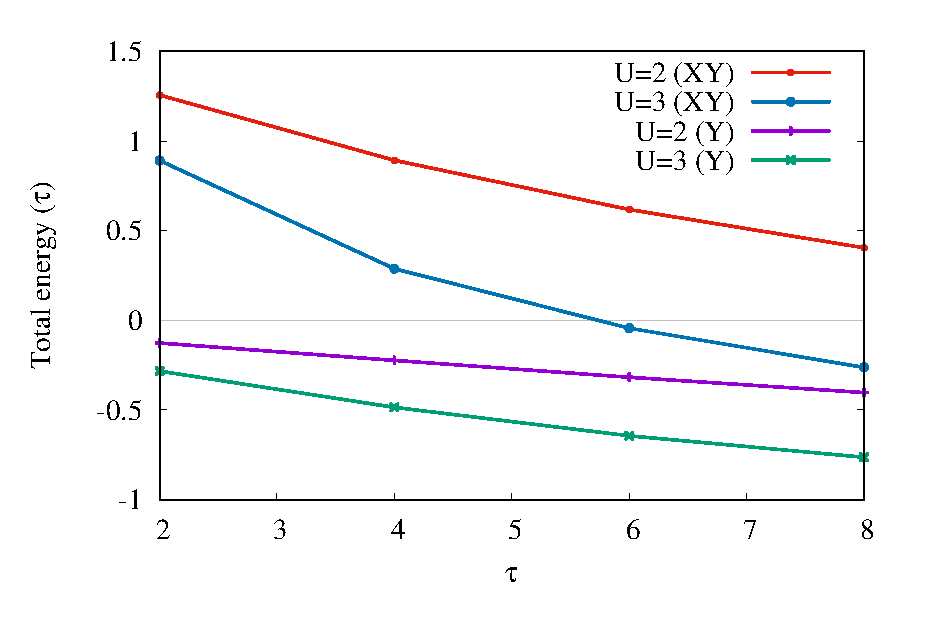
\includegraphics[width=0.7\linewidth]{Chapters/1_pi_pulse_tex/figure/xy/E_tau.eps}} \\
\caption{The total energy after the pulse as a function of the pulse width.}
\label{fig:E_tot_tau}
\end{figure}
%\clearpage

The total energy after the half-cycle pulse as a function of pulse width depicted in Fig.~\ref{fig:E_tot_tau}. For the pulse with $\tau = 2$ ($XY$-polarization), the total energy has a positive and maximum value (red and blue lines), this pulse narrowest in the calculations. With increasing pulse width, the total energy after the pulse can become negative, as seen on the blue line. This behavior was also demonstrated in the work \citep{PhysRevB.85.155124} for the hypercubic lattice.
In the case of a pulse in the $Y$-polarization, the total energy is always negative. With increasing pulse width, the total energy goes deep into the negative region.
%\subsection{Modification of momentum distribution under half-cycle linear polarized pulse.}

Visually change of an electron population can be traced in the time-dependent momentum distribution. Fig.~\ref{fig:md_u2_t0} shows the momentum distribution of the interacting system ($U=2$) at time $t=0$ when the system is in equilibrium and the field does not affect it.
\begin{figure}[h!]
\center{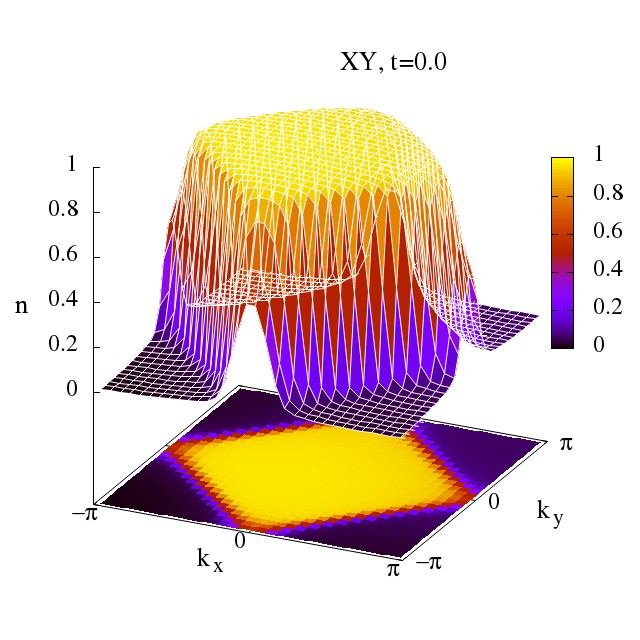
\includegraphics[width=0.5\linewidth]{Chapters/1_pi_pulse_tex/figure/y/A_0.jpg}} \\
\caption{Equilibrium momentum distribution for $U=2$ at $time=0$.}
\label{fig:md_u2_t0}
\end{figure}

\begin{figure}[hp]
\begin{minipage}[h]{0.43\linewidth}
\begin{overpic}[width=1\textwidth]{Chapters/1_pi_pulse_tex/figure/xy/u2/A_200.jpg}
 \put (20,85) {(a)}
\end{overpic}
\end{minipage}
\hfill
\begin{minipage}[h]{0.43\linewidth}
\begin{overpic}[width=1\textwidth]{Chapters/1_pi_pulse_tex/figure/y/u2/A_200.jpg}
 \put (20,85) {(b)}
\end{overpic}
\end{minipage}
\begin{minipage}[h]{0.43\linewidth}
\begin{overpic}[width=1\textwidth]{Chapters/1_pi_pulse_tex/figure/xy/u2/A_300.jpg}
 \put (20,85) {(c)}
\end{overpic}
\end{minipage}
\hfill
\begin{minipage}[h]{0.43\linewidth}
\begin{overpic}[width=1\textwidth]{Chapters/1_pi_pulse_tex/figure/y/u2/A_300.jpg}
 \put (20,85) {(d)}
\end{overpic}
\end{minipage}
\begin{minipage}[h]{0.43\linewidth}
\begin{overpic}[width=1\textwidth]{Chapters/1_pi_pulse_tex/figure/xy/u2/A_400.jpg}
 \put (20,85) {(e)}
\end{overpic}
\end{minipage}
\hfill
\begin{minipage}[h]{0.43\linewidth}
\begin{overpic}[width=1\textwidth]{Chapters/1_pi_pulse_tex/figure/y/u2/A_400.jpg}
 \put (20,85) {(f)}
\end{overpic}
\end{minipage}
\caption{Momentum distribution for $U=2$ at different $time$ $\in$ [2,4], $\tau=4$. Left column (a),(c),(e) - field in $XY$-polarization; right column (b),(d),(f) - field in $Y$-polarization.}
\label{fig:md_u2_A_max}
\end{figure}
%\clearpage



\begin{figure}[hp]
\begin{minipage}[h]{0.43\linewidth}
\begin{overpic}[width=1\textwidth]{Chapters/1_pi_pulse_tex/figure/xy/u2/A_500.jpg}
 \put (20,85) {(a)}
\end{overpic}
\end{minipage}
\hfill
\begin{minipage}[h]{0.43\linewidth}
\begin{overpic}[width=1\textwidth]{Chapters/1_pi_pulse_tex/figure/y/u2/A_500.jpg}
 \put (20,85) {(b)}
\end{overpic}
\end{minipage}
\begin{minipage}[h]{0.43\linewidth}
\begin{overpic}[width=1\textwidth]{Chapters/1_pi_pulse_tex/figure/xy/u2/A_700.jpg}
 \put (20,85) {(c)}
\end{overpic}
\end{minipage}
\hfill
\begin{minipage}[h]{0.43\linewidth}
\begin{overpic}[width=1\textwidth]{Chapters/1_pi_pulse_tex/figure/y/u2/A_700.jpg}
 \put (20,85) {(d)}
\end{overpic}
\end{minipage}
\begin{minipage}[h]{0.43\linewidth}
\begin{overpic}[width=1\textwidth]{Chapters/1_pi_pulse_tex/figure/xy/u2/A_1000.jpg}
 \put (20,85) {(e)}
\end{overpic}
\end{minipage}
\hfill
\begin{minipage}[h]{0.43\linewidth}
\begin{overpic}[width=1\textwidth]{Chapters/1_pi_pulse_tex/figure/y/u2/A_1000.jpg}
 \put (20,85) {(f)}
\end{overpic}
\end{minipage}
\caption{Relaxation of momentum distribution (after pulse) for $U=2$ in different $time$ $\in$ [5,10], $\tau=4$. Left column (a),(c),(e) - $XY$-polarization; right column (b),(d),(f) - $Y$-polarization.}
\label{fig:md_u2_A_max_relaxation}
\end{figure}
%\clearpage






\begin{figure}[hp]
\begin{minipage}[h]{0.43\linewidth}
\begin{overpic}[width=1\textwidth]{Chapters/1_pi_pulse_tex/figure/xy/u3/A_200.jpg}
 \put (20,85) {(a)}
\end{overpic}
\end{minipage}
\hfill
\begin{minipage}[h]{0.43\linewidth}
\begin{overpic}[width=1\textwidth]{Chapters/1_pi_pulse_tex/figure/y/u3/A_200.jpg}
 \put (20,85) {(b)}
\end{overpic}
\end{minipage}
\begin{minipage}[h]{0.43\linewidth}
\begin{overpic}[width=1\textwidth]{Chapters/1_pi_pulse_tex/figure/xy/u3/A_300.jpg}
 \put (20,85) {(c)}
\end{overpic}
\end{minipage}
\hfill
\begin{minipage}[h]{0.43\linewidth}
\begin{overpic}[width=1\textwidth]{Chapters/1_pi_pulse_tex/figure/y/u3/A_300.jpg}
 \put (20,85) {(d)}
\end{overpic}
\end{minipage}
\begin{minipage}[h]{0.43\linewidth}
\begin{overpic}[width=1\textwidth]{Chapters/1_pi_pulse_tex/figure/xy/u3/A_400.jpg}
 \put (20,85) {(e)}
\end{overpic}
\end{minipage}
\hfill
\begin{minipage}[h]{0.43\linewidth}
\begin{overpic}[width=1\textwidth]{Chapters/1_pi_pulse_tex/figure/y/u3/A_400.jpg}
 \put (20,85) {(f)}
\end{overpic}
\end{minipage}
\caption{Momentum distribution for $U=3$ in different $time$ $\in$ [2,4], $\tau=4$. Left column (a),(c),(e) - $XY$-polarization; right column (b),(d),(f) - $Y$-polarization.}
\label{fig:md_u3_A_max}
\end{figure}
%\clearpage


\begin{figure}[h!]
\begin{minipage}[h]{0.43\linewidth}
\begin{overpic}[width=1\textwidth]{Chapters/1_pi_pulse_tex/figure/xy/u3/A_500.jpg}
 \put (20,85) {(a)}
\end{overpic}
\end{minipage}
\hfill
\begin{minipage}[h]{0.43\linewidth}
\begin{overpic}[width=1\textwidth]{Chapters/1_pi_pulse_tex/figure/y/u3/A_500.jpg}
 \put (20,85) {(b)}
\end{overpic}
\end{minipage}
\begin{minipage}[h]{0.43\linewidth}
\begin{overpic}[width=1\textwidth]{Chapters/1_pi_pulse_tex/figure/xy/u3/A_700.jpg}
 \put (20,85) {(c)}
\end{overpic}
\end{minipage}
\hfill
\begin{minipage}[h]{0.43\linewidth}
\begin{overpic}[width=1\textwidth]{Chapters/1_pi_pulse_tex/figure/y/u3/A_700.jpg}
 \put (20,85) {(d)}
\end{overpic}
\end{minipage}
\caption{Relaxation of momentum distribution (after pulse) for $U=3$ in $time=5$ and $time=7$, $\tau=4$. Left column (a),(c) - $XY$-polarization; right column (b),(d) - $Y$-polarization.}
\label{fig:md_u3_A_max_relaxation}
\end{figure}

Under the influence of the half-cycle cosine electric field, the momentum distribution begins to move in the direction of the vector potential (or opposite to the direction of the electric field). Figs.~\ref{fig:md_u2_A_max} shows the momentum distribution for $U=2$ during the action of the pulse. The pulse exists at $time \in $ [0,4] ($\tau=4$). 

In the $XY$-polarization of the field (Figs.~\ref{fig:md_u2_A_max}a,c,e), the shift and flattening of the momentum distribution are seen. This shift leads to an inversion of the population since the maximum of the momentum distribution at the final instant of $time=4$ is at the corners of the first Brillouin zone and the minimum at the $\Gamma$-point. This finite distribution does not change much after the pulse (Figs.~\ref{fig:md_u2_A_max_relaxation}a,c,e). Also, in Fig.~\ref{fig:E_tot}a is presented that after the pulse, the total energy is positive.

Under the $Y$-polarized field, momentum distribution shifts to the value of the vector potential (Figs.~\ref{fig:md_u2_A_max}b,d,f) and has a long relaxation time (Figs.~\ref{fig:md_u2_A_max_relaxation}b,d,f) in comparison with the $XY$-polarization (Figs.~\ref{fig:md_u2_A_max_relaxation}a,c,e).

In Figs.~\ref{fig:md_u3_A_max} is shown momentum distribution for $U=3$ during the action of the pulse. In the $XY$-polarization (Figs.~\ref{fig:md_u3_A_max}a,c,e), the shift which leads to inversion of the population and flattening of the momentum distribution could be observed (Fig. \ref{fig:md_u3_A_max_relaxation}a,c). The distribution after exitation does not change. In Fig.~\ref{fig:E_tot}a is presented that after the pulse the total energy is positive but less than in the case of $U=2$. For $Y$-polarization there is no population inversion (Figs.~\ref{fig:md_u3_A_max}b,d,f) and has a short relaxation time after pulse (Figs.~\ref{fig:md_u3_A_max_relaxation}b,d).



\begin{figure}[hp]
\begin{minipage}[h]{0.43\linewidth}
\begin{overpic}[width=1\textwidth]{Chapters/1_pi_pulse_tex/figure/xy/u2_08A/A_200.jpg}
 \put (20,85) {(a)}
\end{overpic}
\end{minipage}
\hfill
\begin{minipage}[h]{0.43\linewidth}
\begin{overpic}[width=1\textwidth]{Chapters/1_pi_pulse_tex/figure/y/u2_08A/A_200.jpg}
 \put (20,85) {(b)}
\end{overpic}
\end{minipage}
\begin{minipage}[h]{0.43\linewidth}
\begin{overpic}[width=1\textwidth]{Chapters/1_pi_pulse_tex/figure/xy/u2_08A/A_300.jpg}
 \put (20,85) {(c)}
\end{overpic}
\end{minipage}
\hfill
\begin{minipage}[h]{0.43\linewidth}
\begin{overpic}[width=1\textwidth]{Chapters/1_pi_pulse_tex/figure/y/u2_08A/A_300.jpg}
 \put (20,85) {(d)}
\end{overpic}
\end{minipage}
\begin{minipage}[h]{0.43\linewidth}
\begin{overpic}[width=1\textwidth]{Chapters/1_pi_pulse_tex/figure/xy/u2_08A/A_400.jpg}
 \put (20,85) {(e)}
\end{overpic}
\end{minipage}
\hfill
\begin{minipage}[h]{0.43\linewidth}
\begin{overpic}[width=1\textwidth]{Chapters/1_pi_pulse_tex/figure/y/u2_08A/A_400.jpg}
 \put (20,85) {(f)}
\end{overpic}
\end{minipage}
\caption{Momentum distribution for $U=2$ and $0.8A_{max}$ in different $time$ $\in$ [2,4], $\tau=4$. Left column (a),(c),(e) - $XY$ field polarization; right column (b),(d),(f) - $Y$ field polarization.}
\label{fig:md_u2_08A}
\end{figure}
%\clearpage


\begin{figure}[hp]
\begin{minipage}[h]{0.43\linewidth}
\begin{overpic}[width=1\textwidth]{Chapters/1_pi_pulse_tex/figure/xy/u2_08A/A_500.jpg}
 \put (20,85) {(a)}
\end{overpic}
\end{minipage}
\hfill
\begin{minipage}[h]{0.43\linewidth}
\begin{overpic}[width=1\textwidth]{Chapters/1_pi_pulse_tex/figure/y/u2_08A/A_500.jpg}
 \put (20,85) {(b)}
\end{overpic}
\end{minipage}
\begin{minipage}[h]{0.43\linewidth}
\begin{overpic}[width=1\textwidth]{Chapters/1_pi_pulse_tex/figure/xy/u2_08A/A_700.jpg}
 \put (20,85) {(c)}
\end{overpic}
\end{minipage}
\hfill
\begin{minipage}[h]{0.43\linewidth}
\begin{overpic}[width=1\textwidth]{Chapters/1_pi_pulse_tex/figure/y/u2_08A/A_700.jpg}
 \put (20,85) {(d)}
\end{overpic}
\end{minipage}
\begin{minipage}[h]{0.43\linewidth}
\begin{overpic}[width=1\textwidth]{Chapters/1_pi_pulse_tex/figure/xy/u2_08A/A_1000.jpg}
 \put (20,85) {(e)}
\end{overpic}
\end{minipage}
\hfill
\begin{minipage}[h]{0.43\linewidth}
\begin{overpic}[width=1\textwidth]{Chapters/1_pi_pulse_tex/figure/y/u2_08A/A_1000.jpg}
 \put (20,85) {(f)}
\end{overpic}
\end{minipage}
\caption{Relaxation of momentum distribution (after pulse) for $U=2$ and $0.8A_{max}$ in different $time$ $\in$ [5,10], $\tau=4$. Left column (a),(c),(e) - $XY$ field polarization; right column (b),(d),(f) - $Y$ field polarization.}
\label{fig:md_u2_08A_relaxation}
\end{figure}

With increasing interaction, the momentum distribution becomes flattered for all polarizations. It can be associated not only with the correlation effects, which together with the electric field change the topology of the momentum distribution but also with an increase of the effective temperature of the system.

Increasing the value of the Coulomb interaction reduces the relaxation time of the distribution after radiation. It is clearly seen in comparing with the results of relaxation for the $Y$-polarization for different values of the interaction.

In Figs.~\ref{fig:md_u2_08A} and \ref{fig:md_u2_08A_relaxation} is shown momentum distribution for $U=2$ during the action of the pulse and relaxation. The pulses were used with $0.8A_{max}$. This pulse shape does not allow to shift the momentum distribution in the case of $Y$-polarization from $\Gamma$ to Y and in the $XY$-polarization from $\Gamma$ to M in the Brillouin zone during the pulse (Figs.~\ref{fig:md_u2_08A}e,f).


In the process of relaxation (Figs.~\ref{fig:md_u2_08A_relaxation}a,c,e) the minimum of the momentum distribution shifted to the $\Gamma$ point for $XY$-polarization. It takes place because the system needs to adjust the momentum shift to $\pi\sqrt{2}$ to achieve a thermal state. The distribution relax to the thermal states with $T_{eff} < 0$.
As expected, field with $Y$-polarization does not turn over distribution of electrons (Figs.~\ref{fig:md_u2_08A_relaxation}b,d,f).

\vspace{5mm} %5mm vertical space

Thus the geometry of the 2D square lattice gives us the opportunity to investigate the polarization dependence of physical quantity. Due to this fact, the behavior of the system under the action of linearly polarized fields in $XY$ and $Y$-polarization was considered.

In the case of $XY$-polarization, many effects have been found that agreed with the article \citep{PhysRevB.85.155124} such as population inversion and the behavior of relaxation of the momentum distribution to the thermal state in case of the non-optimal vector potential. 

The population inversion is not observed at the considered parameters of the laser pulse and the Coulomb interaction for the $Y$-polarization. It is shown in the graphs of the total energy, double occupancy, and the momentum distribution. The distribution has a long relaxation time compared with the results for the $XY$ pulse polarization. 





\FloatBarrier
\section{Population inversion induced by a circularly polarized pulse}

In the paragraph, we examine in detail how the sign of the interaction changes in the presence of a circularly polarized field on the 2D square lattice. 

Selecting the pulse parameters possible to change interaction from repulsive to attractive by different scenarios. For this purpose, we use half- mono- and multi-cycle circularly polarized pulses with different lattice and pulse parameters. 

\subsection{Monocycle pulse condition}

Consider the transition from linear to circular polarization for a half-cycle pulse. Figs.~\ref{fig:Pulses_3} shows the graphs of vector potentials. 
\begin{figure}[h!]
\begin{minipage}[h]{0.5\linewidth}
\center{\includegraphics[width=1\linewidth]{Chapters/1_pi_pulse_tex/figure_c/3/Pulse_1.eps}} (a) \\
\end{minipage}
\begin{minipage}[h]{0.5\linewidth}
\center{\includegraphics[width=1\linewidth]{Chapters/1_pi_pulse_tex/figure_c/3/Pulse_4.eps}} \\(b)
\end{minipage}
\caption{Circularly polarized vector potentials with different phases between $X$ and $Y$ projections: (a) $\phi_y=\pi /4$; (b) $\phi_y=\pi /2$.}
\label{fig:Pulses_3}
\end{figure}
The trajectory of the center of momentum distribution is shown in Fig.~\ref{fig:Pulse_p_3}. The trajectory strongly depends on the polarization and the amplitude of the $X$ and $Y$ component of the vector potential. The curves with phase between $X$ and $Y$ projections equal to $\phi_y=\pi /4$ corresponds to circular polarization, $\phi_y=\pi /3$ and $\phi_y=5\pi /12$ are elliptical and phase equal to $\phi_y=\pi /2$ has linear polarization.

The monocycle condition:
\begin{equation}
\text{FWHM}={1 \over \omega}\\
\label{eq:monocycle_condition}
\end{equation}
were FWHM - full width at half maximum, $\omega$ - frequency.
\begin{figure}[h!]
\center{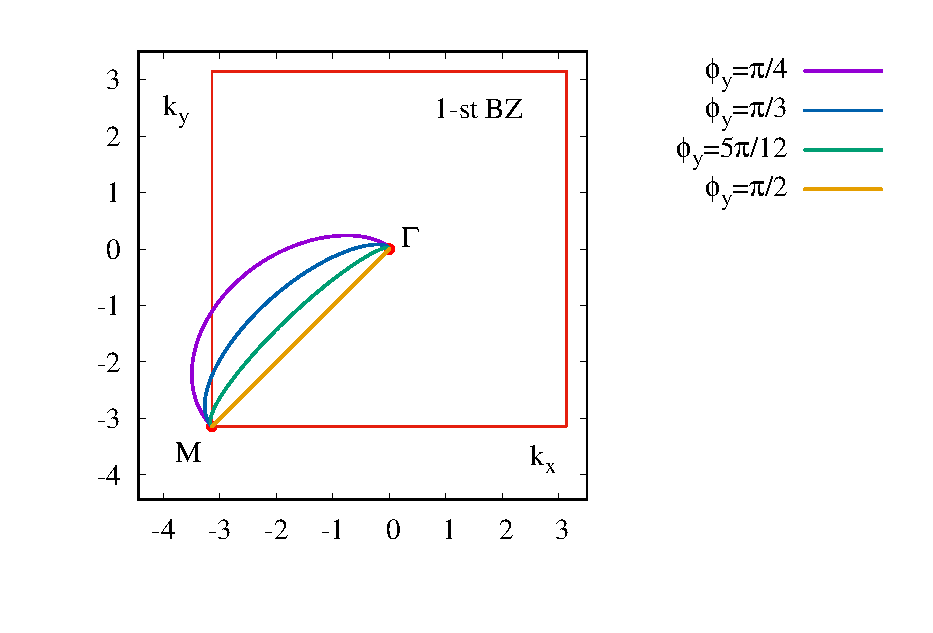
\includegraphics[width=0.7\linewidth]{Chapters/1_pi_pulse_tex/figure_c/3/Pulse_p.eps}} \\
\caption{Middle point trajectories of the momentum distribution for different phases between $X$ and $Y$ projections of the vector potential.}
\label{fig:Pulse_p_3}
\end{figure}

\begin{figure}[h!]
\begin{minipage}[h]{0.5\linewidth}
\center{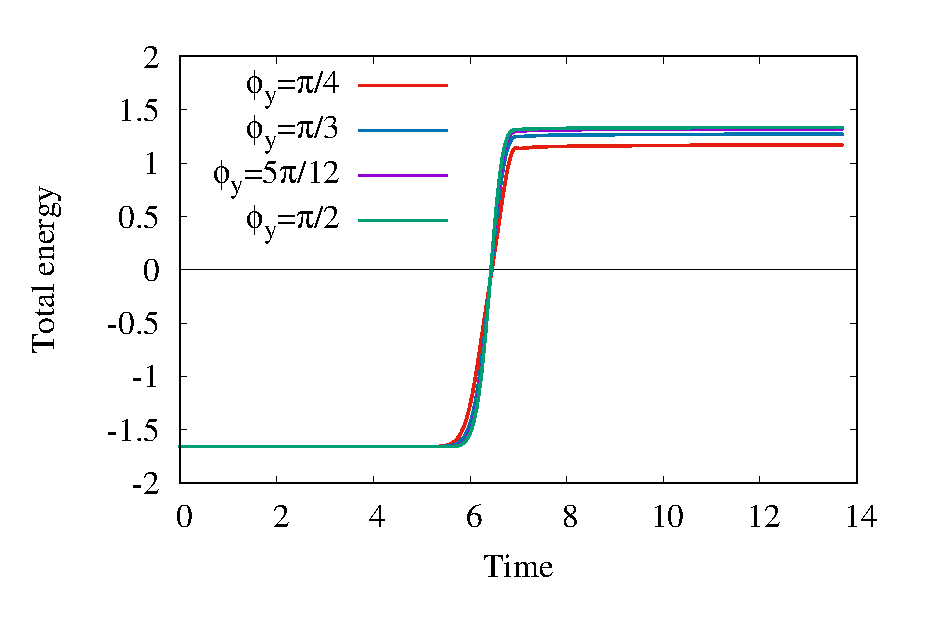
\includegraphics[width=1\linewidth]{Chapters/1_pi_pulse_tex/figure_c/3/Etot.eps}} (a) \\
\end{minipage}
\hfill
\begin{minipage}[h]{0.5\linewidth}
\center{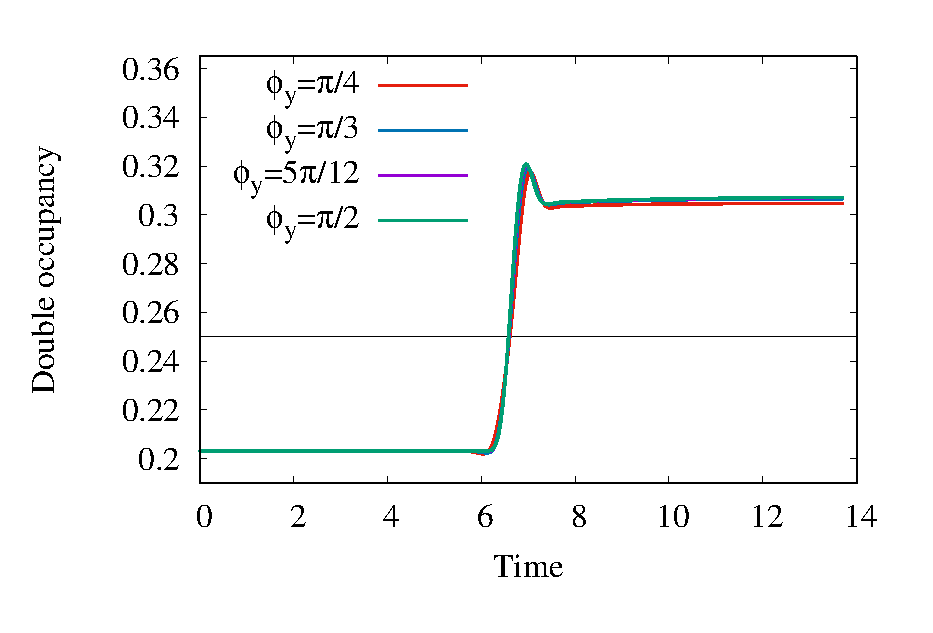
\includegraphics[width=1\linewidth]{Chapters/1_pi_pulse_tex/figure_c/3/docc.eps}} \\(b)
\end{minipage}
\caption{Dependence of the total energy (a) and double occupancy (b) for different phases between $X$ and $Y$ projections of the vector potential.}
\label{fig:Etot_3}
\end{figure}

To obtain a more significant population inversion better to apply the pulse with linear $XY$-polarization; this can be seen from the graph of the total energy in Fig.~\ref{fig:Etot_3}a. Gradually increasing the polarization from linear to circular, the final value of the total energy slightly decreases. But the double occupancy (Fig.~\ref{fig:Etot_3}b) react to the change of phase between the $X$ and $Y$ components of the field polarization not significantly.
\FloatBarrier

%\subsection{The frequency dependence}

Next, consider how the physical parameters of the model change under the action of half-cycle circularly polarized vector potentials with different frequencies. Figs.~\ref{fig:Pulses_2} shows the graphs vector potentials for these cases. 
\begin{figure}[h!]
\begin{minipage}[h]{0.5\linewidth}
\center{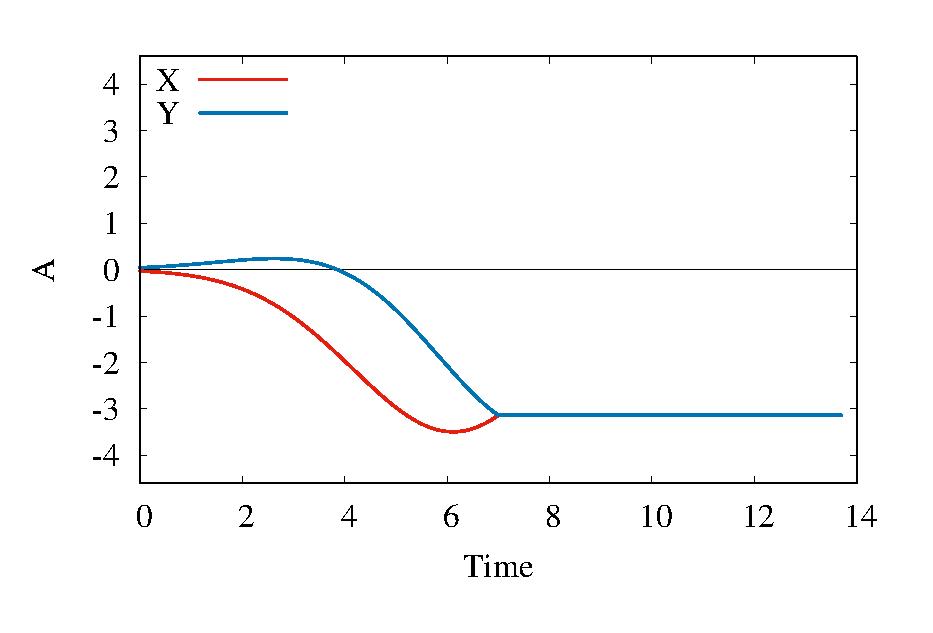
\includegraphics[width=1\linewidth]{Chapters/1_pi_pulse_tex/figure_c/2/Pulse_0.eps}} (a) \\
\end{minipage}
\begin{minipage}[h]{0.5\linewidth}
\center{\includegraphics[width=1\linewidth]{Chapters/1_pi_pulse_tex/figure_c/2/Pulse_4.eps}} \\(b)
\end{minipage}
\caption{Vector potentials with different frequencies: (a) $\omega=0.25$; (b) $\omega=2$.}
\label{fig:Pulses_2}
\end{figure}
%The trajectory of the momentum distribution is the same everywhere for each frequency. Than higher the frequency then faster the momentum distribution moves from the $\Gamma$ point of the Brillouin zone to M. 

Total energy and double occupancy respond strongly to such a frequency change (Fig.~\ref{fig:Etot_2}). The higher the frequency of the pulse, the greater the total energy and double occupancy, and therefore the greater the population inversion.
%\begin{figure}[h!]
%\center{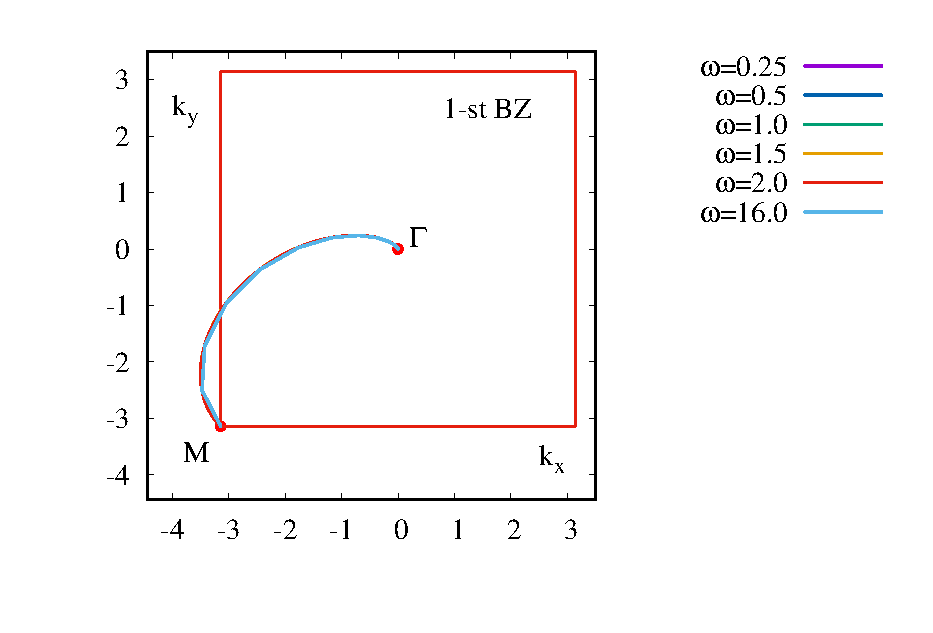
\includegraphics[width=0.7\linewidth]{Chapters/1_pi_pulse_tex/figure_c/2/Pulse_p.eps}} \\
%\caption{Middle point trajectories of the momentum distribution for different frequencies of the vector potential.}
%\label{fig:Pulse_p_2}
%\end{figure}
\begin{figure}[h!]
\begin{minipage}[h]{0.5\linewidth}
\center{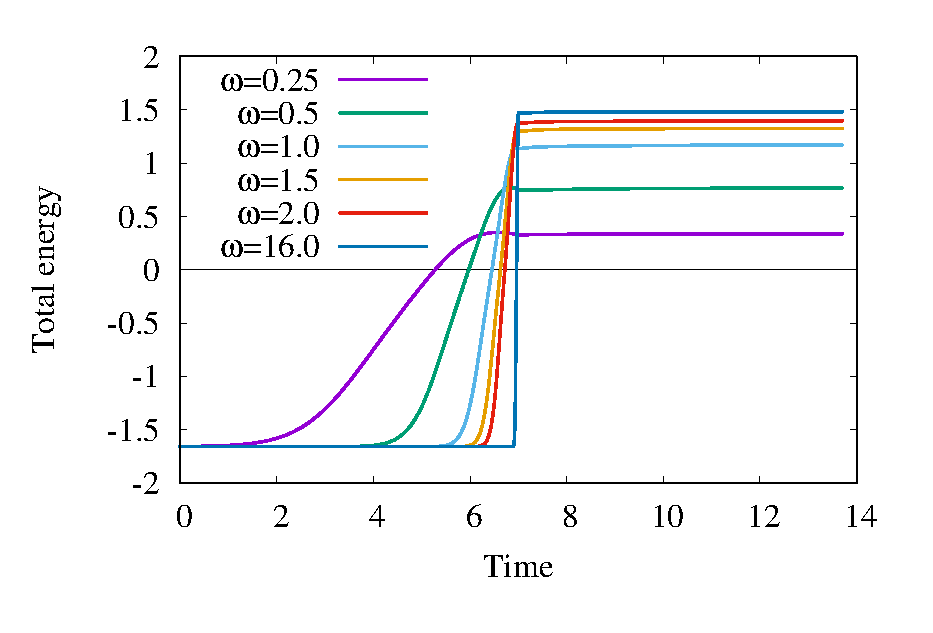
\includegraphics[width=1\linewidth]{Chapters/1_pi_pulse_tex/figure_c/2/Etot.eps}} (a) \\
\end{minipage}
\hfill
\begin{minipage}[h]{0.5\linewidth}
\center{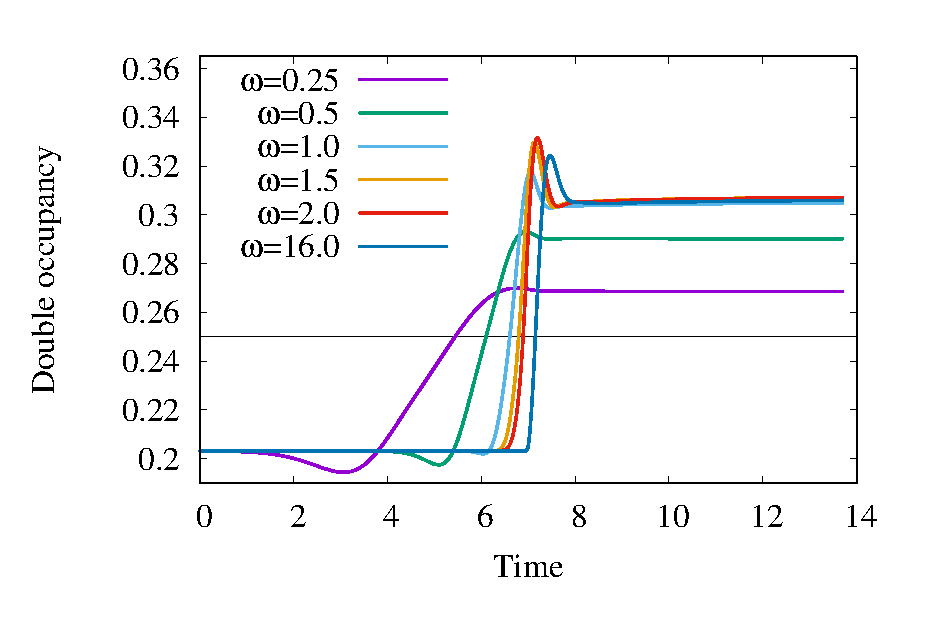
\includegraphics[width=1\linewidth]{Chapters/1_pi_pulse_tex/figure_c/2/docc.eps}} \\(b)
\end{minipage}
\caption{Dependence of the total energy (a) and double occupancy (b) from the frequency of the vector potential.}
\label{fig:Etot_2}
\end{figure}

In Figs.~\ref{fig:md_2} depicted the behavior of the momentum distribution in the circular field at different points in time for $U=2$. Distribution moves in the direction of the vector potential at $time=5.0$ to $time=7.0$ because electric field is switched on (Figs.~\ref{fig:md_2}a-d). After $time=7.0$ the distribution stop moving because process of relaxation starts and until $time=10.0$ the topology becomes smoother.
\begin{figure}[h!]
\begin{minipage}[h]{0.43\linewidth}
\begin{overpic}[width=1\textwidth]{Chapters/1_pi_pulse_tex/figure_c/2/A_550.jpg}
 \put (20,85) {(a)}
\end{overpic}
\end{minipage}
\hfill
\begin{minipage}[h]{0.43\linewidth}
\begin{overpic}[width=1\textwidth]{Chapters/1_pi_pulse_tex/figure_c/2/A_700.jpg}
 \put (20,85) {(d)}
\end{overpic}
\end{minipage}
\begin{minipage}[h]{0.43\linewidth}
\begin{overpic}[width=1\textwidth]{Chapters/1_pi_pulse_tex/figure_c/2/A_600.jpg}
 \put (20,85) {(b)}
\end{overpic}
\end{minipage}
\hfill
\begin{minipage}[h]{0.43\linewidth}
\begin{overpic}[width=1\textwidth]{Chapters/1_pi_pulse_tex/figure_c/2/A_750.jpg}
 \put (20,85) {(e)}
\end{overpic}
\end{minipage}
\begin{minipage}[h]{0.43\linewidth}
\begin{overpic}[width=1\textwidth]{Chapters/1_pi_pulse_tex/figure_c/2/A_650.jpg}
 \put (20,85) {(c)}
\end{overpic}
\end{minipage}
\hfill
\begin{minipage}[h]{0.43\linewidth}
\begin{overpic}[width=1\textwidth]{Chapters/1_pi_pulse_tex/figure_c/2/A_1000.jpg}
 \put (20,85) {(f)}
\end{overpic}
\end{minipage}
\caption{Momentum distribution for $U=2$ in different $time$ $\in$ [5.5,10] with $\omega=1$ and FWHM=1.}
\label{fig:md_2}
\end{figure}

\FloatBarrier

%\subsection{Circular monocycle pulse with different initial phases.}

Consider how the properties of the Hubbard model change under the influence of monocycle pulses at different values of the initial phase (Fig.~\ref{fig:Pulses_1}).
\begin{figure}[h!]
\begin{minipage}[h]{0.5\linewidth}
\center{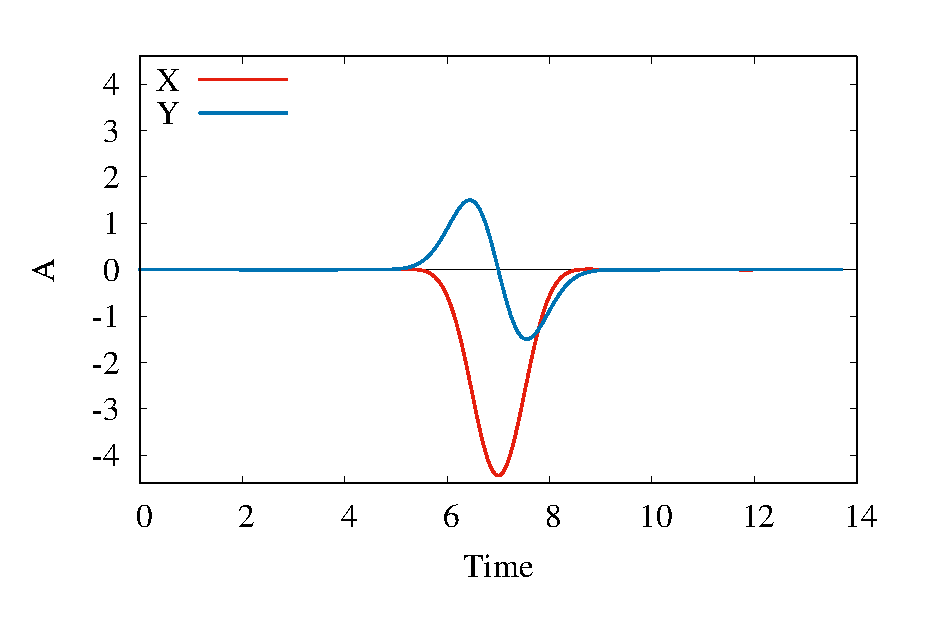
\includegraphics[width=1\linewidth]{Chapters/1_pi_pulse_tex/figure_c/1/u_0/Pulse_1.eps}} (a) \\
\end{minipage}
\hfill
\begin{minipage}[h]{0.5\linewidth}
\center{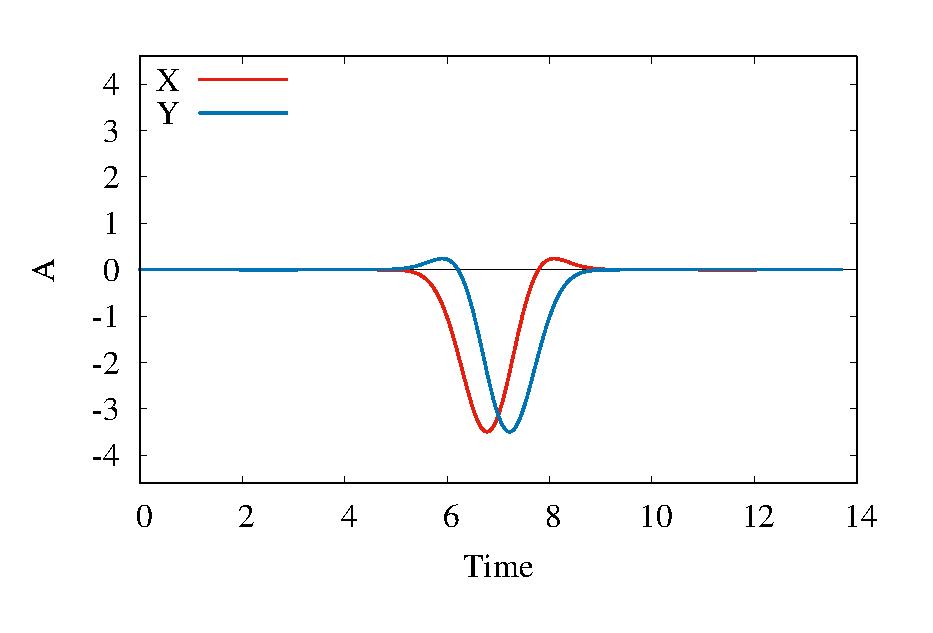
\includegraphics[width=1\linewidth]{Chapters/1_pi_pulse_tex/figure_c/1/u_0/Pulse_3.eps}} \\(c)
\end{minipage}
\begin{minipage}[h]{0.5\linewidth}
\center{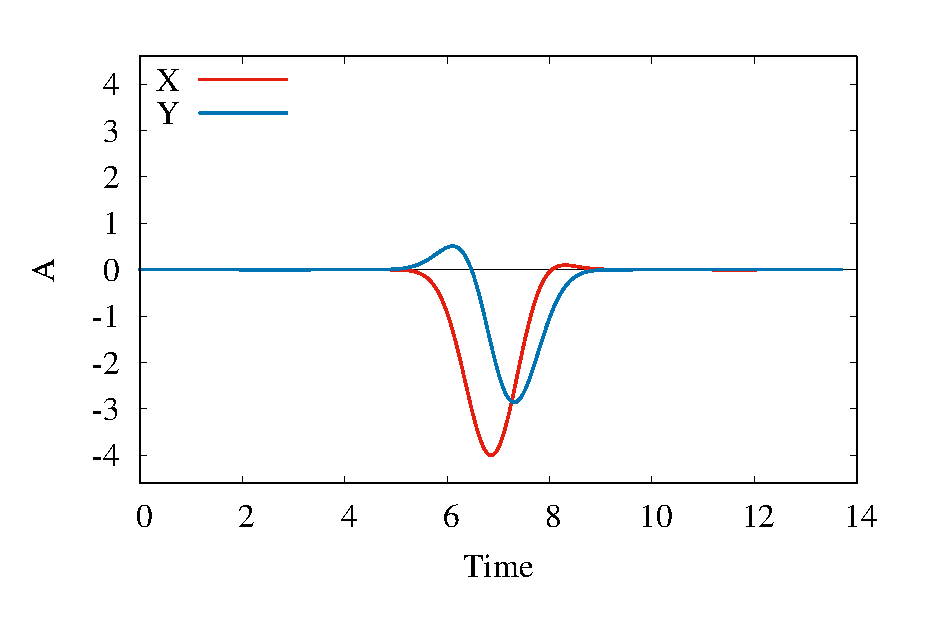
\includegraphics[width=1\linewidth]{Chapters/1_pi_pulse_tex/figure_c/1/u_0/Pulse_2.eps}} (b) \\
\end{minipage}
\hfill
\begin{minipage}[h]{0.5\linewidth}
\center{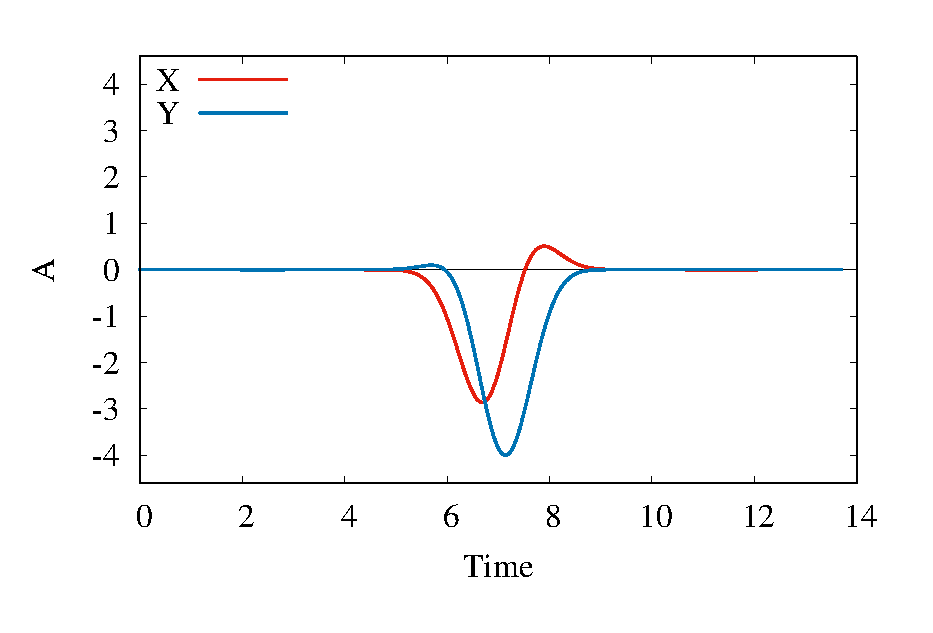
\includegraphics[width=1\linewidth]{Chapters/1_pi_pulse_tex/figure_c/1/u_0/Pulse_4.eps}} \\(d)
\end{minipage}
\caption{Vector potentials with different initial phases: (a) $\phi_y=0$; (b) $\phi_y=\pi /6$; (c) $\phi_y=\pi /4$; (d) $\phi_y=\pi /3$.}
\label{fig:Pulses_1}
\end{figure}

Moving the maximum of the momentum distribution from $\Gamma$ point of the Brillouin zone to the M point is depicted in Fig.~\ref{fig:Pulse_p_1}. 

Figs.~\ref{fig:Etot_1} shows the total energy and double occupancy for different values of the initial phases of the vector potential and for various Coulomb interactions $U$. Fig.~\ref{fig:Etot_1}a depicts the total energy for a pulse at $U=0$. The maximum value of the total energy is reached for $\phi_y=\pi /4$. The total energy for $\phi_y=\pi /6$ and $\phi_y=\pi /3$ are symmetrical relative to the middle of the pulse ($time=7$) and graph for $\phi_y=0$ symmetrical since it is always equidistant from M points of the Brillouin zone during the whole pulse time (Fig.~\ref{fig:Pulse_p_1} red line). The double occupancy (Fig.~\ref{fig:Etot_1}a) is equal to $0.25$ during all time, which must be in case of $U=0$.


\begin{figure}[h!]
\center{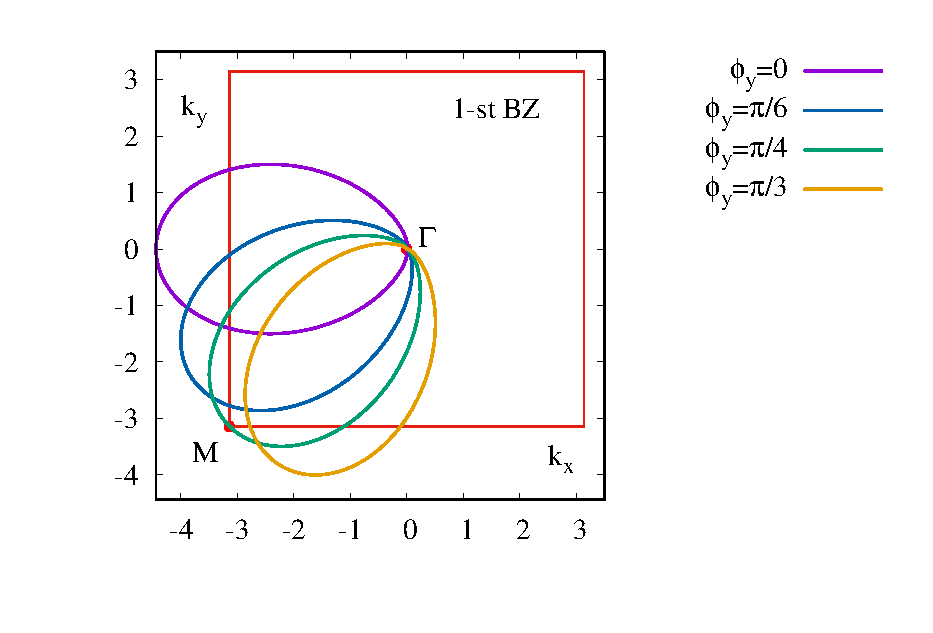
\includegraphics[width=0.7\linewidth]{Chapters/1_pi_pulse_tex/figure_c/1/u_0/Pulse_p.eps}} \\
\caption{Middle point trajectories of the momentum distribution with different initial phases of the vector potential.}
\label{fig:Pulse_p_1}
\end{figure}
Figs. \ref{fig:Etot_1}b,d show the total energy and double occupancy for a monocycle pulse at different initial phases in the case of $U=2$. The symmetry of the total energy with respect to the middle of the pulse disappears gradually depending on the magnitude of interaction.

All considered pulses lead to population inversion. The total energy for $\phi_y=\pi /6$ and $\phi_y=\pi /3$ are not any more symmetrical relative to the middle of pulse $time=7$. The curve at $\phi_y=\pi /6$ has a bigger maximum of the total energy comparing to $\phi_y=\pi /3$. Increasing the interaction lead to increasing of an energy absorption by the system and thus it increases the temperature during the pulse. The temperature rise makes the flatter momentum distribution that reduces the value of the population inversion, because more electrons are now may extend to the edges of the "hat" of the momentum distribution. At the same time, as it shown by previous calculations, the form of the "hat" of the momentum distribution for the correlated system itself may vary during the pulse. Thus, competition of the effects: inclusion of correlations that tend to bend the "hat" of the momentum distribution, shifting the momentum distribution by the vector potential to a more "favorable" position and heating the system, may explain why we see the maximum value of the total energy and double occupancy for the pulse with $\phi_y=\pi /3$ slightly larger than for $\phi_y=\pi /4$ in Figs.~\ref{fig:Etot_1}b,d.
\begin{figure}[h!]
\begin{minipage}[h]{0.5\linewidth}
\center{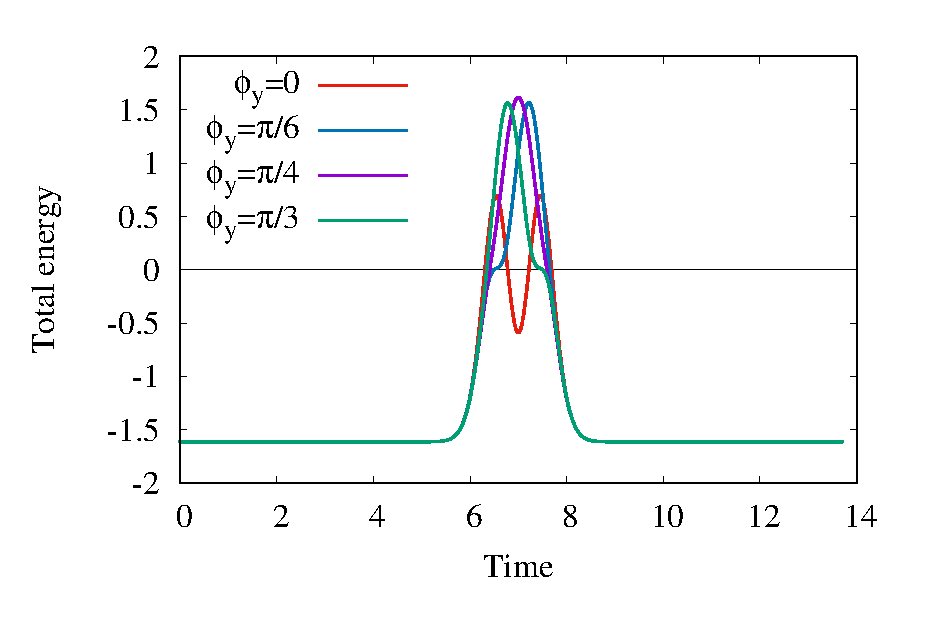
\includegraphics[width=1\linewidth]{Chapters/1_pi_pulse_tex/figure_c/1/u_0/Etot.eps}} (a) \\
\end{minipage}
\hfill
\begin{minipage}[h]{0.5\linewidth}
\center{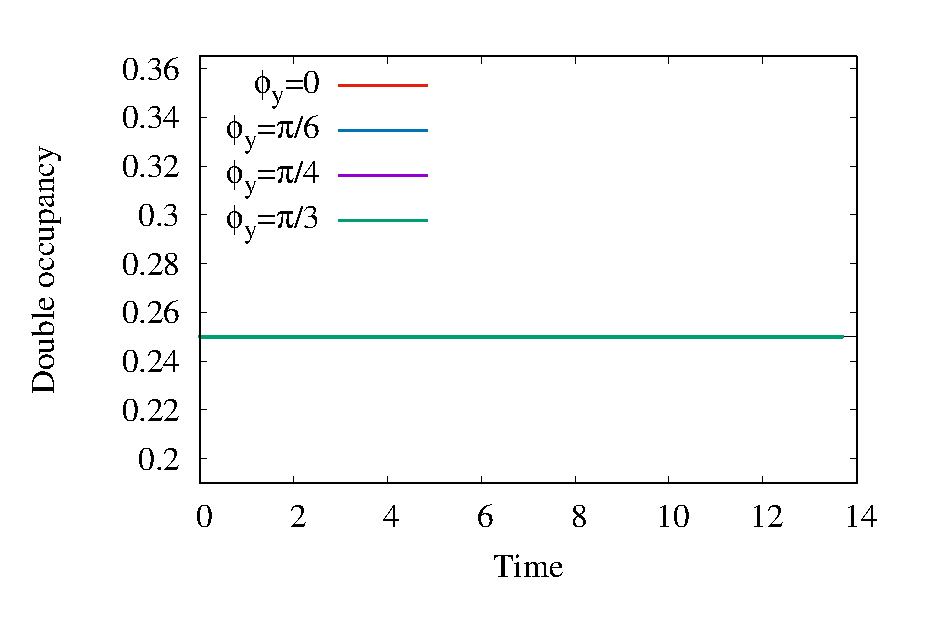
\includegraphics[width=1\linewidth]{Chapters/1_pi_pulse_tex/figure_c/1/u_0/docc.eps}} \\(c)
\end{minipage}
\begin{minipage}[h]{0.5\linewidth}
\center{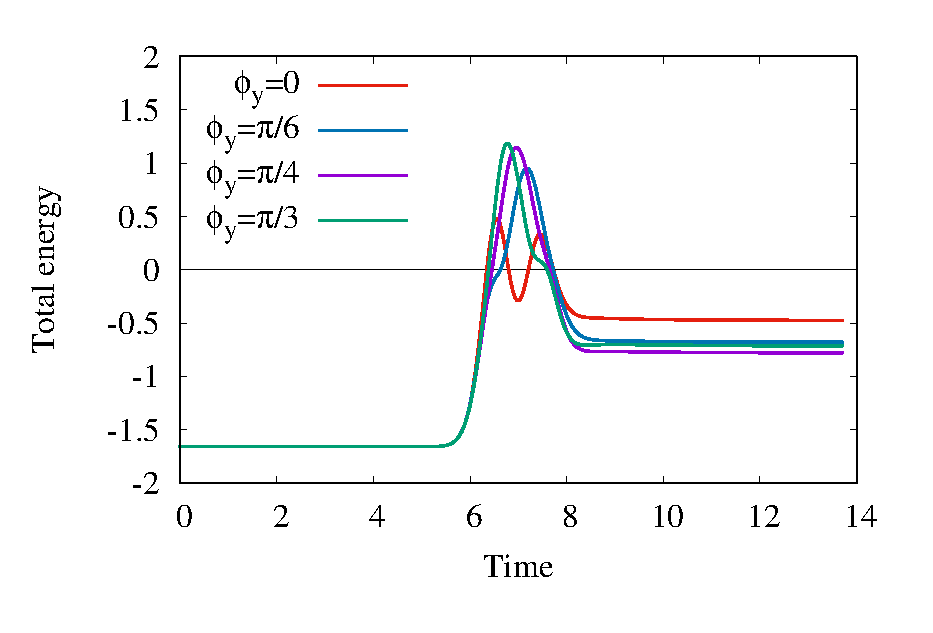
\includegraphics[width=1\linewidth]{Chapters/1_pi_pulse_tex/figure_c/1/u_2/Etot.eps}} (b) \\
\end{minipage}
\hfill
\begin{minipage}[h]{0.5\linewidth}
\center{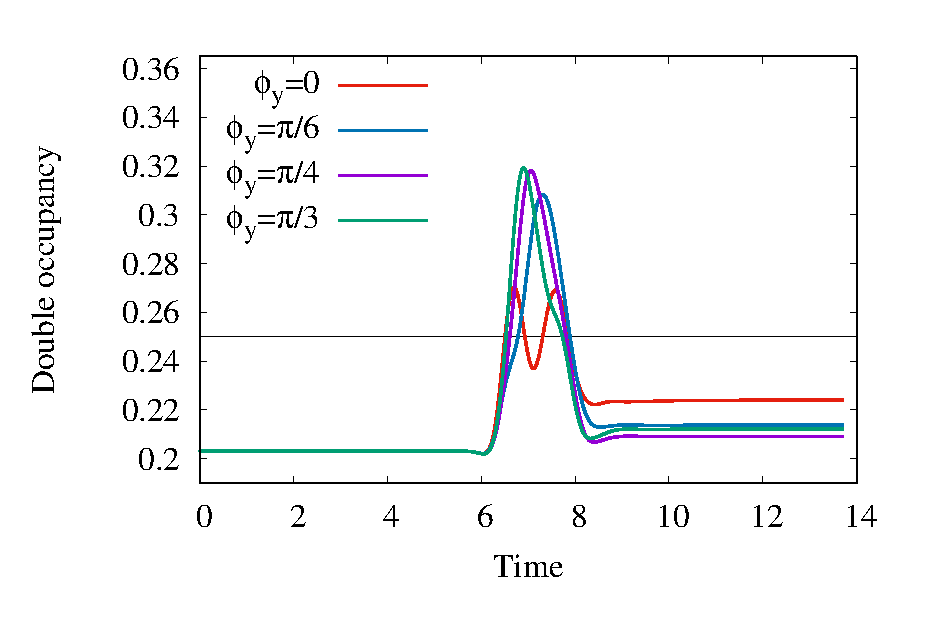
\includegraphics[width=1\linewidth]{Chapters/1_pi_pulse_tex/figure_c/1/u_2/docc.eps}} \\(d)
\end{minipage}
\caption{Dependence of total energy and double occupancy from different initial phases of the vector potential: (a),(c) case of $U=0$; (b),(d) case of $U=2$.}
\label{fig:Etot_1}
\end{figure}

\FloatBarrier

\subsection{Beyond of monocycle condition}

It is interesting to explore how the model behaves outside of the monocycle condition. Fig.~\ref{fig:Pulses_4} shows the graphs of half-cycle circularly polarized vector potentials with different ratios FWHM and $\omega$.
\begin{figure}[h!]
\begin{minipage}[h]{0.5\linewidth}
\center{\includegraphics[width=1\linewidth]{Chapters/1_pi_pulse_tex/figure_c/4/Pulse_1.eps}} (a) \\
\end{minipage}
\hfill
\begin{minipage}[h]{0.5\linewidth}
\center{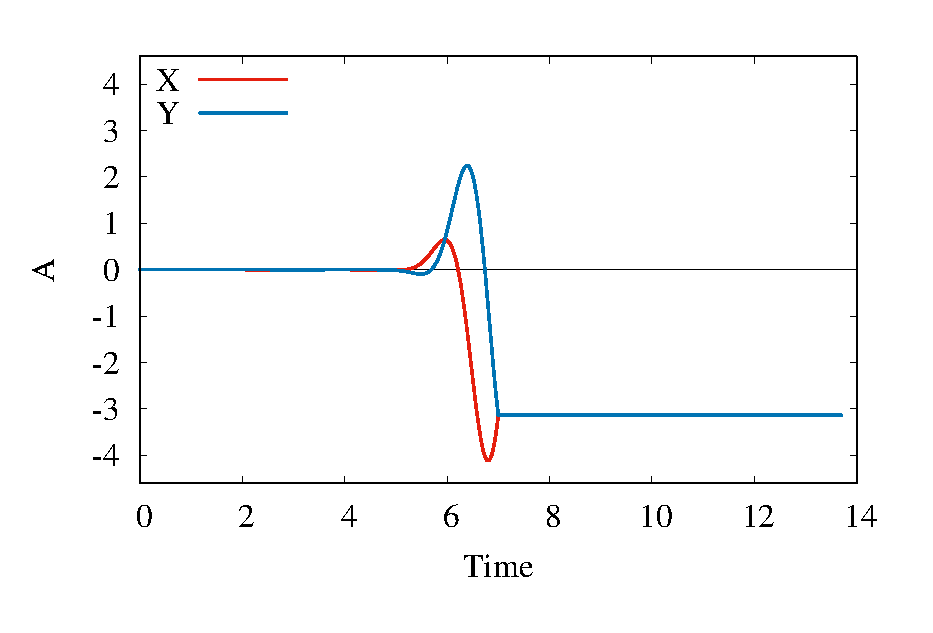
\includegraphics[width=1\linewidth]{Chapters/1_pi_pulse_tex/figure_c/4/Pulse_3.eps}} \\(c)
\end{minipage}
\begin{minipage}[h]{0.5\linewidth}
\center{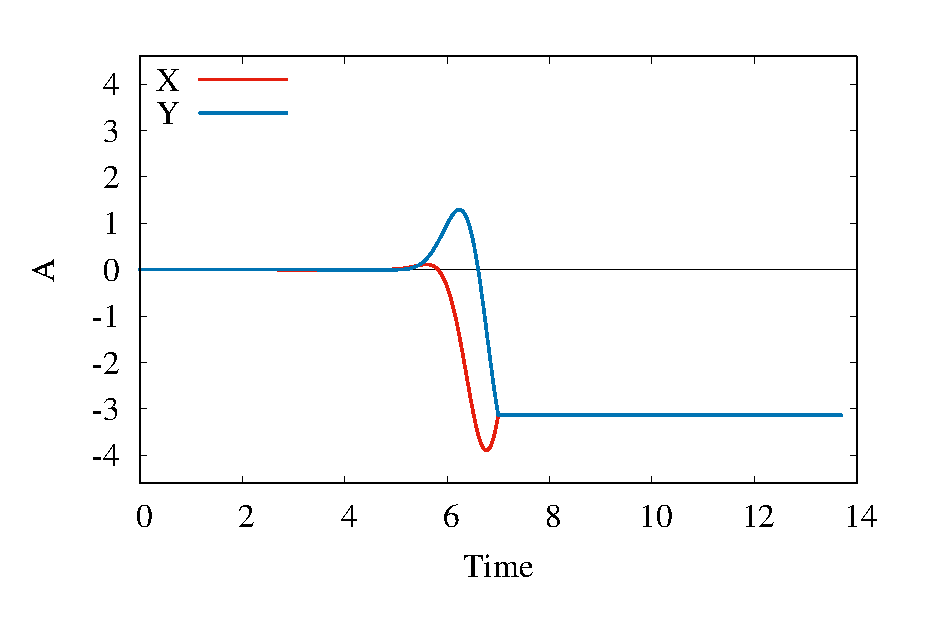
\includegraphics[width=1\linewidth]{Chapters/1_pi_pulse_tex/figure_c/4/Pulse_2.eps}} (b) \\
\end{minipage}
\hfill
\begin{minipage}[h]{0.5\linewidth}
\center{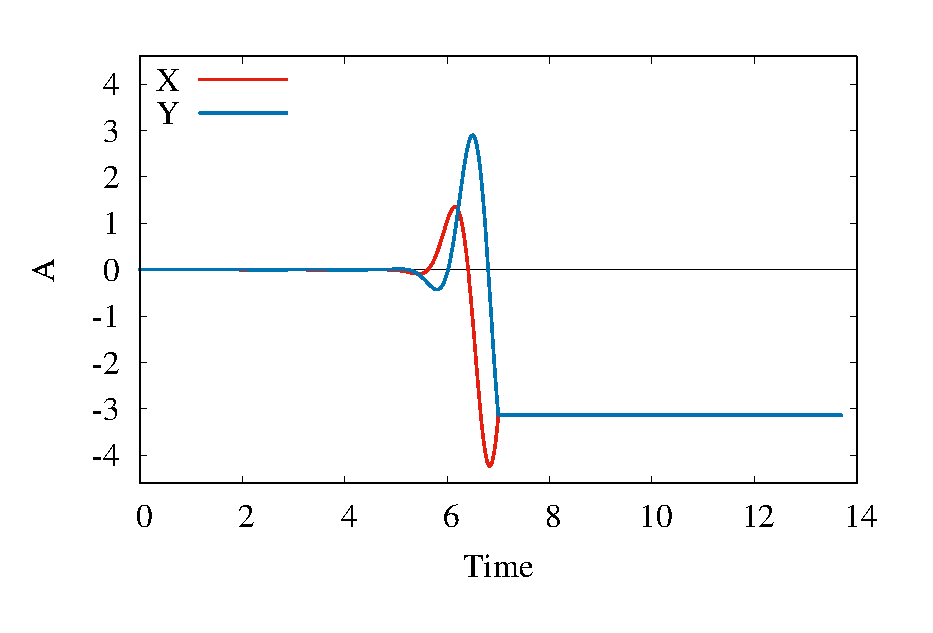
\includegraphics[width=1\linewidth]{Chapters/1_pi_pulse_tex/figure_c/4/Pulse_4.eps}} \\(d)
\end{minipage}
\caption{Vector potentials for different frequencies with fixed FWHM: (a) $\omega=1.0$ monocycle condition; (b) $\omega=2.0$; (c) $\omega=3.0$; (d) $\omega=4.0$.}
\label{fig:Pulses_4}
\end{figure}

By increasing the frequency of the pulse and leaving the FWHM constant we move away from the monocycle condition Eq.~\eqref{eq:monocycle_condition}. Fig.~\ref{fig:Pulse_p_4} illustrate trajectory of the center momentum distribution for $\pi$-pulse. Line with $\omega=1$ is a half-cycle pulse with the monocycle condition.
\begin{figure}[h!]
\center{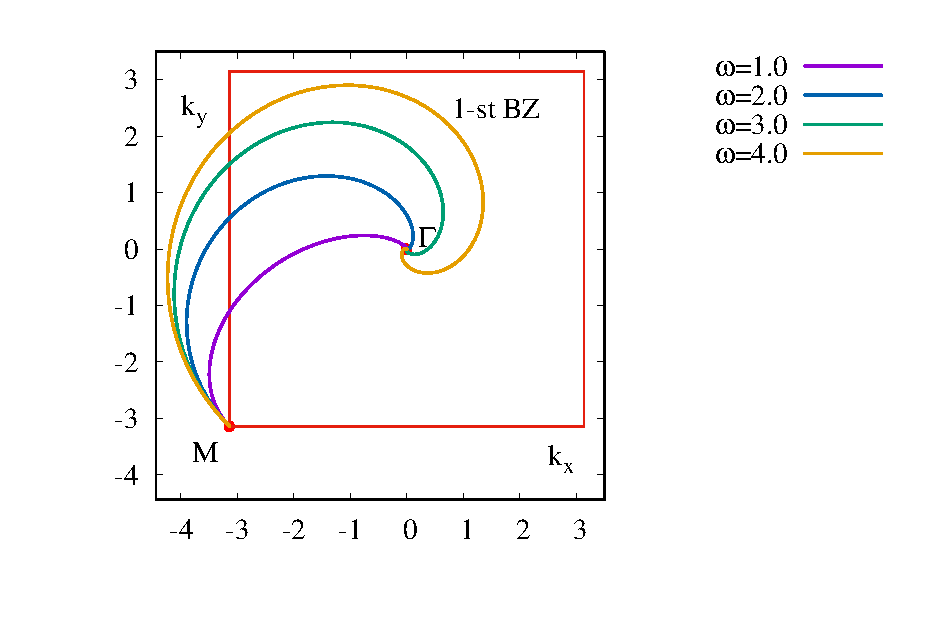
\includegraphics[width=0.7\linewidth]{Chapters/1_pi_pulse_tex/figure_c/4/Pulse_p.eps}} \\
\caption{Middle point trajectories of the momentum distribution for different frequencies with fixed FWHM of the vector potentials.}
\label{fig:Pulse_p_4}
\end{figure}

The total energy of such pulses (Fig.~\ref{fig:Etot_4}a) has a different structure during the excitation, nevertheless the optimal inversion presented at the $\pi$-pulse with the monocycle condition. This can be explained by the fact that the monocycle condition has the shortest way to move the center of momentum distribution from $\Gamma$ to M point, which contributes to less heating of the system. 
\begin{figure}[h!]
\begin{minipage}[h]{0.5\linewidth}
\center{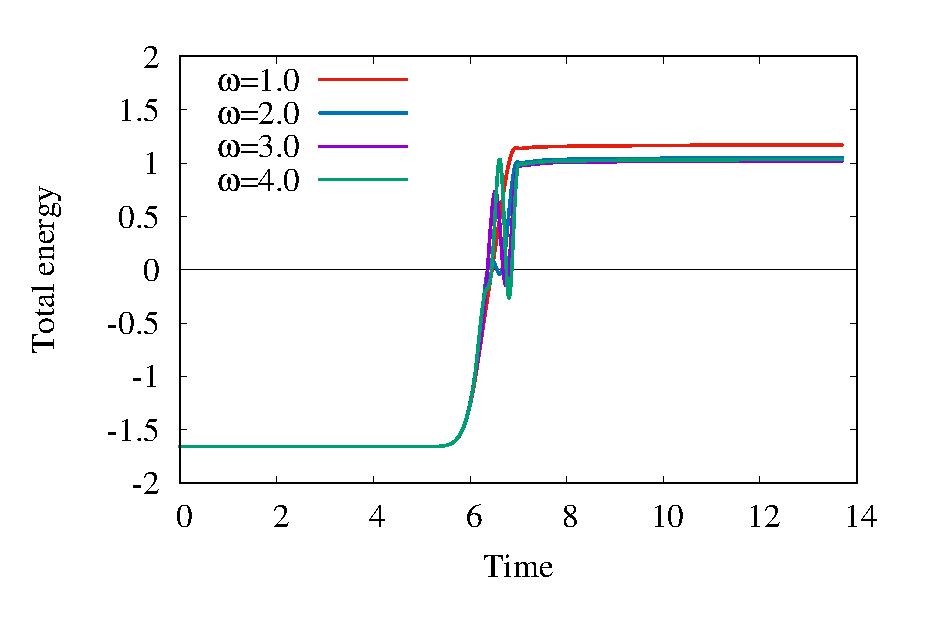
\includegraphics[width=1\linewidth]{Chapters/1_pi_pulse_tex/figure_c/4/Etot.eps}} (a) \\
\end{minipage}
\hfill
\begin{minipage}[h]{0.5\linewidth}
\center{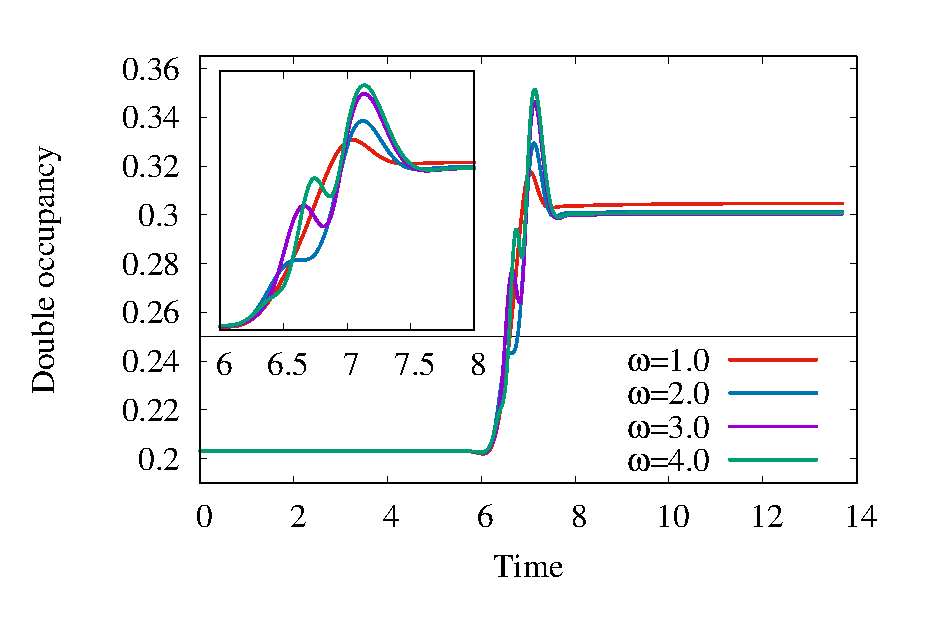
\includegraphics[width=1\linewidth]{Chapters/1_pi_pulse_tex/figure_c/4/docc.eps}} \\(b)
\end{minipage}
\caption{Dependence of the total energy (a) and double occupancy (b) from different frequencies with fixed FWHM of the vector potentials.}
\label{fig:Etot_4}
\end{figure}

Beyond of the monocycle condition Eq. \eqref{eq:monocycle_condition}  additional peak appears in the graphs of total energy and double occupancy (Fig.~\ref{fig:Etot_4}). The peak gradient increases and moves towards greater times. The presence of the peak at these graphs is due to the fact that the center of momentum distribution in the non-monocycle case passes near another M point in the first Brillouin zone, thereby creating an inversion on that part of the trajectory. 

\FloatBarrier

\subsection{Multicycle pulse}

In this part, we discuss how to create a maximum population inversion during multicycle circularly polarized pulse. A ramp of the vector potential is depicted in Fig.~\ref{fig:Pulses_5}. The maximum amplitude of the vector potential is $A_{max}=4.44$. 
\begin{figure}[h!]
\center{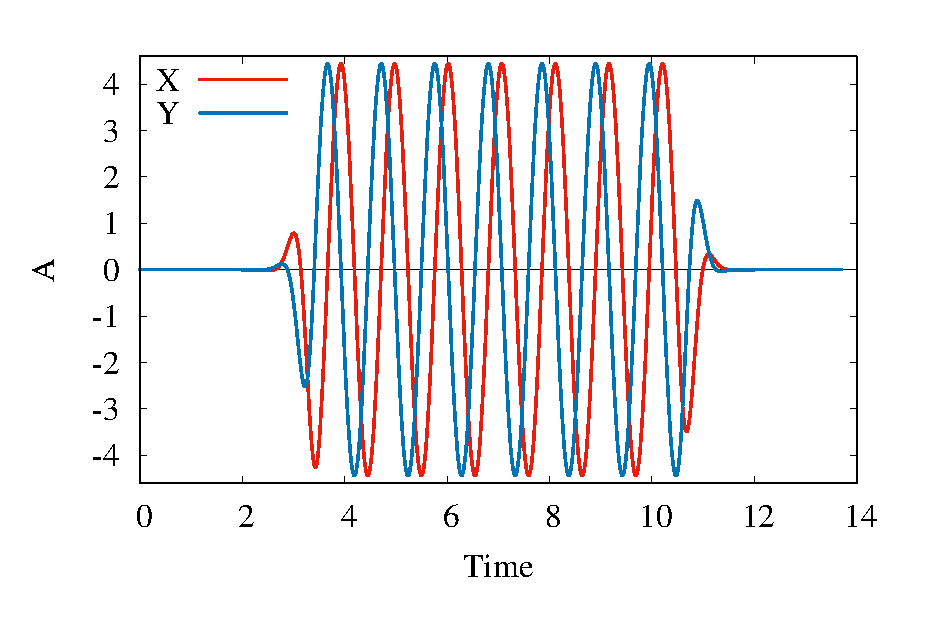
\includegraphics[width=0.55\linewidth]{Chapters/1_pi_pulse_tex/figure_c/plot/Pulse_3.eps}} \\
\caption{The ramp of the multicycle circularly polarized vector potential.}
\label{fig:Pulses_5}
\end{figure}

This form of vector potential that moves the middle of the momentum distribution from $\Gamma$ through all four M points in the 2D square lattice in Brillouin zone (Fig. \ref{fig:Pulse_p_5}).
\begin{figure}[h!]
\center{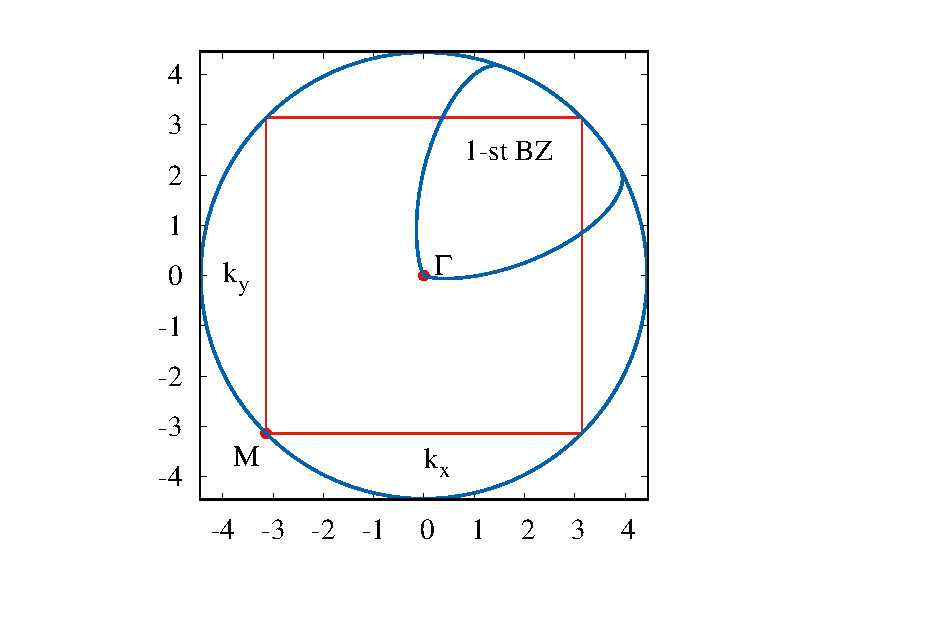
\includegraphics[width=0.7\linewidth]{Chapters/1_pi_pulse_tex/figure_c/plot/Pulse_p_w1.eps}} \\
\caption{Middle point trajectories of the momentum distribution induced by the ramp of the multicycle circularly polarized vector potential.}
\label{fig:Pulse_p_5}
\end{figure}

The corresponding total energy and double occupancy are shown in Fig.~\ref{fig:Etot_5}. General patterns characterize results for all frequencies. Initially, the total energy increases from negative to positive value, then oscillates and finally decreases to the negative. The behavior of the double occupancy is very similar, except that it can only be positive and grows to a higher value than 0.25.
This corresponds to the fact that the maximum of the momentum distribution first goes from the $\Gamma$ point to a circle close to the M point (Fig.~\ref{fig:Pulse_p_5}). Moving in a circle near all four M points inversion of the population occurs, and over the X and Y points in the BZ it disappears. 

\clearpage

\begin{figure}[h!]
\begin{minipage}[h]{0.5\linewidth}
\begin{overpic}[width=1\textwidth]{Chapters/1_pi_pulse_tex/figure_c/plot/Etot_1.eps}
 \put (22,55) {(a)}
\end{overpic}
\end{minipage}
\hfill
\begin{minipage}[h]{0.5\linewidth}
\begin{overpic}[width=1\textwidth]{Chapters/1_pi_pulse_tex/figure_c/plot/docc_1.eps}
 \put (24,55) {(d)}
\end{overpic}
\end{minipage}
\begin{minipage}[h]{0.5\linewidth}
\begin{overpic}[width=1\textwidth]{Chapters/1_pi_pulse_tex/figure_c/plot/Etot_2.eps}
 \put (22,55) {(b)}
\end{overpic}
\end{minipage}
\hfill
\begin{minipage}[h]{0.5\linewidth}
\begin{overpic}[width=1\textwidth]{Chapters/1_pi_pulse_tex/figure_c/plot/docc_2.eps}
 \put (24,55) {(e)}
\end{overpic}
\end{minipage}
\begin{minipage}[h]{0.5\linewidth}
\begin{overpic}[width=1\textwidth]{Chapters/1_pi_pulse_tex/figure_c/plot/Etot_3.eps}
 \put (22,55) {(c)}
\end{overpic}
\end{minipage}
\hfill
\begin{minipage}[h]{0.5\linewidth}
\begin{overpic}[width=1\textwidth]{Chapters/1_pi_pulse_tex/figure_c/plot/docc_3.eps}
 \put (24,55) {(f)}
\end{overpic}
\end{minipage}
%\begin{minipage}[h]{0.5\linewidth}
%\begin{overpic}[width=1\textwidth]{Chapters/1_pi_pulse_tex/figure_c/%plot/Etot_4.eps}
% \put (22,55) {(d)}
%\end{overpic}
%\end{minipage}
%\hfill
%\begin{minipage}[h]{0.5\linewidth}
%\begin{overpic}[width=1\textwidth]{Chapters/1_pi_pulse_tex/figure_c/%plot/docc_4.eps}
% \put (24,55) {(h)}
%\end{overpic}
%\end{minipage}
\caption{Dependence of the total energy (a-c) left column and corresponded double occupancy (d-f) right column, at $U=2$ from different frequencies ($\omega=1$;$3$ and $6$) of the multicycle circularly polarized vector potential.}
\label{fig:Etot_5}
\end{figure}
And finally, at the end of the pulse, the maximum of distribution returns to its initial location at the $\Gamma$ point, but it has already been changed by the effects of correlations, external field, and temperature.
As the pulse frequency increases, the total energy tends to oscillate and be in the majority with a positive value. The higher the field frequency, the longer it remains in transient positive value. The double occupancy fully arrives above 0.25 at the time of the excitations for frequencies above $\omega=1$. 

The total energy and double occupancy at high frequencies of the external field initially have a change in the amplitude of oscillations. However, after some time, the mean value and amplitude of oscillations hardly change. This implies that we detect a transition to a mode where physical observables are periodic in time what can be connected with the Floquet regime.

%\vspace{5mm} %5mm vertical space
\FloatBarrier
\section{Summary}
Thus, summarizing the various options for changing the sign of the interaction in the Hubbard model under the influence of the external field, we come to the following conclusions:

1. Creating of the population inversion becomes more efficient in linear pulse compare to circularly polarized (Fig.~\ref{fig:Etot_3}a).

2. Higher pulse frequency helps to significantly increase inversion in the case of $\pi$-pulse (Fig.~\ref{fig:Etot_2}).

3. With the circularly polarized vector potential, the maximum positive value of the total energy depends on the initial phase as well. To create population inversion, do not necessary to have a phase due to which the middle of momentum distribution is transferred exactly from the $\Gamma$ point to M, as previously expected. This case is shown in Fig.~\ref{fig:Etot_1}b.

4. Moving away from the monocycle condition for circular polarization allows creating controlled peaks of the total energy that can change the sign of the interaction (Fig.~\ref{fig:Etot_4}a).

5. It is important to note how the parameters of the system and the pulse separately affect the distribution. In equilibrium, correlations and temperature blur the Fermi step, the electric field used as a vector potential shift the distribution by the value of this vector potential. In nonequilibrium in the absence of correlations, the momentum distribution moves in the direction of the vector potential without changing its shape. 
The momentum distribution distorted under the action of the combined effects of correlations, the electric field (for all considered polarization) and an increasing of the effective temperature.
%\begin{frontmatter}



%\title{Tuning properties of strongly correlated materials by means of strong laser pulses}% Force line breaks with \\
% \title{Post-Floquet engineering of electronic phase transitions by intense laser pulses}
\chapter{Strongly correlated Kramers-Henneberger solid}
\label{chap:KH_solid}
Strong laser electric fields exert forces on an electron comparable to forces binding the electron to an atomic core. Surprisingly, 
such strong fields do not always destroy the atom, but may rather create new bound electronic states residing in a new potential generated by the combined action of the laser field and the core. This so-called "Kramers-Henneberger atom" has recently been observed experimentally, settling decades of debate regarding its existence. 
Here we show that similar novel electronic structures can appear in strongly correlated solids. In our system, the effective potential generated by the laser-induced many-body dynamics traps the electrons, converting metallic into an insulating phase. The electron interaction is crucial to establish this Kramers-Henneberger solid. After the pulse is over the system remains in a state of high electronic temperature, which still has insulating (or rather a bad metallic) properties.
Our finding demonstrates new ways of manipulating phases 
of correlated systems with strong, non-resonant low-frequency 
fields, opening a new regime of "post-Floquet" engineering of strongly correlated systems. 



\section{Introduction}

Light is a powerful and versatile tool for controlling the properties of quantum systems. Exquisite control over light fields, available today, opens an opportunity to shape electronic states by
tailoring the light field, aiming to obtain "properties on demand" \citep{Basov}. 
Already at modest laser intensities, simple non-resonant shifts of atomic energy levels offer an extraordinary control tool, leading to optical traps, optical lattices, tweezers, \cite{Gao_1} etc. At higher intensities, the concept of a "dressed atom" embodies the appearance of new light-induced Floquet states, 
representing "matter + light" hybrid states with sidebands separated by the photon energy. 
These have led to new phenomena, from 
efficient laser cooling leading to 
Bose-Einstein condensation, to electromagnetically induced transparency and related phenomena, to Floquet engineering of quantum matter, e.g. using light to turn a trivial insulator into a topological \cite{Oka_Aoki_1,Kitamura_AR_2019,Huebener_1}. 
The Floquet states for time-periodic modulations are a temporal analog of the Bloch states for spatially periodic potentials.

At still higher laser intensities, the photon-counting inherent 
in the frequency-domain Floquet picture loses its simplicity -- 
too many photons are constantly exchanged between the field and the system. A welcome alternative is offered by the time-domain picture, which explicitly incorporates
the sub-cycle response of charges to the oscillating electric field. 
One example pertinent to our work is the so-called Kramers-Henneberger (KH) atom, where an intense laser field dominates the electron motion \cite{Popov_1,Henneberger_1,Gavrila_1}. The electron oscillates as nearly free so that the field-free electronic density is changed completely. 
It acquires a characteristic double-peak structure, 
with the peaks concentrated near the turning points of the 
oscillatory trajectory. The atomic core keeps the electron from drifting away, and the strongest attraction
arises when one of the two turning points is positioned 
near the core, leading to the formation of long-lived states
with a characteristic double-peaked structure.
The emergence of the Kramers-Henneberger atom leads to 
spectacular effects, from
accelerating neutral atoms at rates $\sim 10^{15}$m/s$^2$ in 
intense laser fields, to the exponential amplification of visible radiation generated
during propagation of intense infrared light in dense gases,
at the frequencies absent in the spectrum of the field-free 
gas \cite{Matthews_1}.
\begin{figure}[h!]
\begin{minipage}[h]{0.5\linewidth}
\center{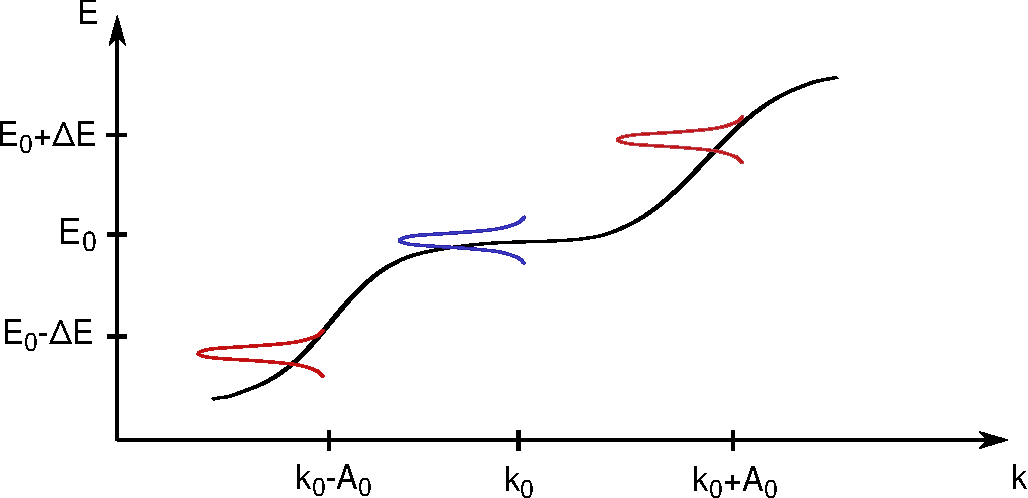
\includegraphics[width=1\linewidth]{Chapters/KH_solid/Band_sketch_1_1.pdf}} (a) \\
\end{minipage}
\hfill
\begin{minipage}[h]{0.5\linewidth}
\center{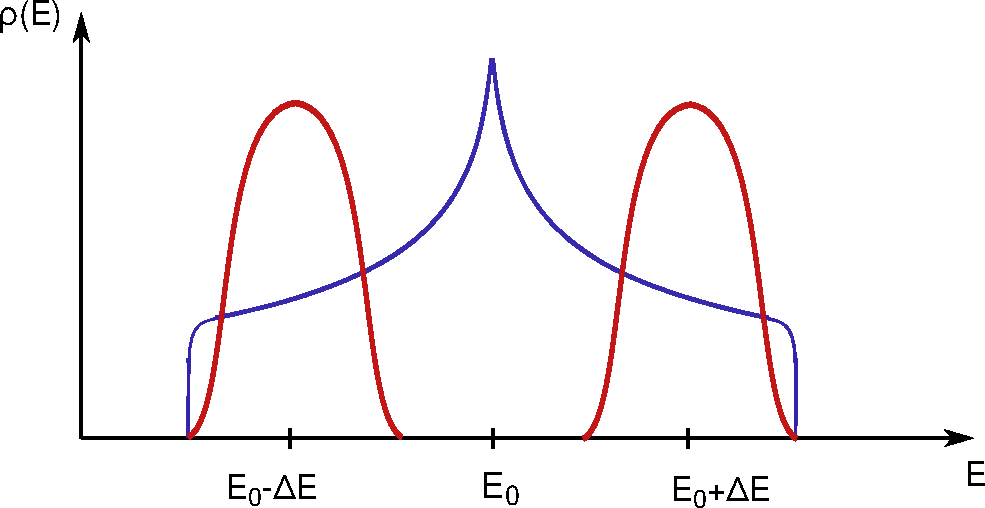
\includegraphics[width=1\linewidth]{Chapters/KH_solid/DOS_sketch_2_1.pdf}} (b) \\
\end{minipage}
\caption{Schematic band structure of square lattice. Pulse with vector potential amplitude $A_0$ drive the electrons with initial momentum $\bf k_0$ from high-density region $\text{E}_0$ to regions with momentum $\bf k_{0} \pm A_0$ and energy $\text{E}_{0}\pm\Delta\text{E}$.}
\label{BandPulse}
\end{figure}

Now we can question what will happen if we turn from an atom to electrons in solids. Fig.\ref{BandPulse} sketches the qualitative idea of extending the KH
perspective to a correlated solid modeled as a half-filled tight-binding electron model with the 
hopping rate $t_{ij}$ on a square lattice with the Hubbard-type (on-site) electron-electron repulsion $U$.
The field-free system is in the correlated metallic phase\cite{RevModPhys.68.13}, below a Mott metal-insulator transition, with the van Hove singularity 
in the density of states at the Fermi level (with the crystal momentum 
${\bf k}_0=0$, Fig.~\ref{BandPulse}a).
As the laser is turned on, it induces a current and drives the 
electrons away from the van Hove singularity to the turning
points along the dispersion curve ${\bf k}_{0} \pm {\bf A}_0$ and energy $\text{E}_{0}\pm\Delta\text{E}$ 
where
${\bf A}_0=F_0/\omega$ the amplitude of the field vector-potential
(Fig.~\ref{BandPulse}a) and $F_0, \omega$ being the field amplitude and
frequency, respectively, while $\Delta\text{E}$ defined by complicated combinations of correlation effects, a band dispersion and pulse parameters.


%This motion already in the non-interacting case has the potential to 
%transform the charge distribution from the 
%single peak near the van Hove
%singularity at the Fermi level into a double-peaked structure 
%near the turning points of the electron 
%trajectory (Fig.~\ref{BandPulse}b). 

%To induce similar modification in a 
%correlated Hubbard system and convert its metallic
%phase into insulating, the interaction with the laser field 
%should lead to the strong reduction of the 
%effective hopping rate $t_{ij}$ in the dressed system.
%This could change the system from the metallic to
%the Mott-insulating state, stabilizing 
%the insulating gap and the doubly-peaked charge distribution 
%imposed by the laser-driven motion (similar to Fig.~\ref{BandPulse}b) and moving the 
%system into an insulating state. 


%In the Floquet formalism, such transition was observed in dynamical mean-field theory and high-frequency expansion\cite{PhysRevB.93.144307,PhysRevB.99.019902}. We will discuss here experimentally realised cases of low-frequency pulses which cannot be treated in the Floquet scheme [see Sec. \ref{beyond_Floquet}].   

The mathematical analogy with the Kramers-Henneberger atom is 
as follows. The KH atom is described by transforming the 
Hamiltonian into the reference frame moving with a free electron,
${\bf r}\rightarrow{\bf r}+{\bf a}(t)$, where ${\bf a}(t)$ describes
laser-driven oscillations of the free electron.
This transformation removes the standard laser-matter interaction 
term in the Hamiltonian while modifying the electron-core interaction potential $U(\bf r)$ to
$U_{\rm KH}({\bf r},t)=U({\bf r}+{\bf a}(t))$.
The new potential exactly incorporates the dominant, laser-induced component of electron dynamics. Next, one expands 
$U_{\rm KH}({\bf r},t)$ in Fourier series.
The zero-frequency term $U^{(0)}_{\rm KH}({\bf r})$, 
which averages $U_{\rm KH}({\bf r},t)$ over the laser cycle, 
is the new effective potential describing the slow
dynamics and the 
bound states of the new system. Other 
Fourier components $U^{(N)}_{\rm KH}({\bf r})\exp(-iN\omega t)$ are responsible
for transitions between the new states. 
In lattices, the analogue of the KH-transformation is 
the Peierls substitution \cite{Peierls1933}, which moves 
the light-matter interaction term into the time-dependence of the 
hopping parameter between cites $i,j$,
\begin{equation}
t_{ij}(t)=t_{ij}\exp(-i{\bf R}_{ij}\cdot {\bf A}(t)),
\end{equation}
with ${\bf R}_{ij}$ the vector connecting the cites and ${\bf A}(t)$
the laser vector-potential. The zero-order term 
in the Fourier expansion of $t_{ij}(t)$, which for
$A(t)=A_0\cos\omega t$ is $t^{(0)}_{ij}
=t_{ij}J_0({\bf R}_{ij} {\bf A}_0)$, is the renormalized hopping rate
(here $J_0(x)$ is the zero-order Bessel function, 
$A_0=F_0/\omega$ is the amplitude of the vector potential along [11] direction in the present case, 
$F_0$ is the electric field amplitude). 
For one-electron systems, this reduction of the hopping rate leads to the well-known coherent destruction of tunneling \cite{Dunlap1986}. 

In spite of the analogy to the KH atom, the cycle-averaged electronic structure in a solid without interactions would in general not give rise to a two-peak structure as illustrated in Fig.~\ref{BandPulse}, because a hopping renormalization in all directions implies only an overall bandwidth renormalization. The essential difference to the atom is that in solid, the spectrum emerges from a superposition of delocalized momentum states such as shown in Fig.~\ref{BandPulse}. Nevertheless, we will demonstrate below the double-peaked charge distribution imposed by the laser-driven motion can be established when the field effect cooperates with the electron interaction. In correlated systems, where the interplay of the hopping rate and the on-site interaction determines the many-body state, even modest reduction in the effective hopping rate can change the system from metallic to Mott-insulating state \cite{RevModPhys.86.779}. Hence, the interaction should cooperate with the field to turn a system of delocalized electrons into a KH solid.


In the Floquet formalism, such transition was observed in dynamical mean-field theory and high-frequency expansion \cite{PhysRevB.93.144307,PhysRevB.99.019902}. We will discuss here experimentally realized cases of low-frequency pulses 
far from the off-resonant limit, 
which cannot be treated in the Floquet scheme.

%In correlated
%systems, where the interplay of the hopping rate and 
%the on-site interaction determines the many-body state, 
%even modest reduction in the effective hopping rate 
%%Mott-insulating state \cite{RevModPhys.86.779}. 
% , stabilizing 
% the insulating gap and the double-peaked charge distribution 
% imposed by the laser-driven motion (Fig.1b) and moving the 
% system into an insulating state

Note that, just like the 
KH-atom does not have to be described solely with 
the cycle-average potential $U^{(0)}_{\rm KH}({\bf r})$, 
the reduction of the hopping rate does not have to be
described solely with 
the cycle-average $t^{(0)}_{ij}$. In general, 
for 
laser frequencies the reduction 
occurs already on the sub-cycle scale\cite{PhysRevB.85.155124} as soon as the laser-induced bias $F_0a_0$ between the neighboring lattice sites ($a_0$ is the lattice constant) becomes comparable to the 
corresponding next-neighbor hopping rate $t_1$; such
sub-cycle perspective becomes particularly relevant 
for the relatively low-frequency fields 
$\omega \ll W, U$, where $W=8t_1$ is the width of the 
first Hubbard band. 

There are, of course, fundamental differences of the KH solid to laser-dressed atoms. Strong laser pulses in metals typically induce a large excitation density, which itself can have a substantial effect on the spectrum in correlated electrons. While there have been proposals to use the field-induced localization of electrons to enhance specific interaction effects in Mott insulators,\cite{dasari2019revealing,Werner_2015} where the electrons are already localized, it is therefore unclear how the KH atom emerges in a system of initially delocalized electrons. Furthermore, while light-induced effects in atoms disappear as soon as the light is turned off, the excitations in the solid can imply a persistent modification of the electronic structure. In insulators or gapped systems, this photo-excitation can generate non-thermal metastable states \cite {PhysRevLett.110.136404,PhysRevB.91.245153}. In metals, excitations typically thermalize within only few hopping times, even in the vicinity of the Mott transition \cite{PhysRevLett.120.166401, PhysRevLett.103.056403}. It should be emphasized that in correlated systems this huge increase in electron temperature can transform a metal into a bad metallic or insulating-like state with a pseudo-gap, and hence imply a modification of the electronic structure which is typically not accessible in equilibrium (because the lattice cannot by heated to correspondingly high temperatures).

%However, there is a fundamental difference between 
%laser-dressed systems such as atoms and a 
%strongly correlated system.
%In atoms, light-induced states disappear as soon as the 
%light is turned off. Here, however, the interplay of a strong  
%laser field and correlated dynamics generates
%a metastable state surviving after the end of the laser pulse.
%The presence of long-lived non-thermal states, which 
%do not relax to the thermal ones after the driving field is switched off \cite {PhysRevLett.110.136404,PhysRevB.91.245153}, is an important property 
%of correlated systems. Intense laser field allows us 
%to access such transient states, which are 
%inaccessible via adiabatic or thermal pathways \cite{RevModPhys.86.779}. 

Highly non-perturbative interaction involving a vast number of photons and generating new system properties after the end of the pulse offers control beyond Floquet engineering.  
In contrast to phonon-driven transitions \cite{Cavalleri_2011}, 
our mechanism is purely electronic, with the effect arising
within a fraction of the cycle of the driving laser field.

\section{Kramers-Henneberger solid}

To demonstrate this qualitative idea quantitatively, 
we consider a two-dimensional, half-filled square 
Fermi-Hubbard lattice interacting with intense,
linearly polarized field. In contrast to previously studied 
Bethe- or hypercube-lattices \cite{PhysRevLett.106.236401,PhysRevB.91.245153} or one-dimensional chains\cite{Rui}, here the field can be applied either along one of the lattice directions, obtaining a quasi one-dimensional system (studied e.g. by Silva et al. \cite{Rui}), or along the diagonal, obtaining the situation similar to the Bethe-lattice or infinite-dimensional hypercube, but with realistic two-dimensional band electron dispersion, including the van Hove singularity at the Fermi level and sharp band step at the edges. To treat the non-perturbative 
time-dependent problem, we used the non-equilibrium 
extension \cite{schmidt2002,RevModPhys.86.779} of 
the Dynamical Mean-Field Theory (DMFT) \cite{RevModPhys.68.13}.
The algorithm and its realization are described in [Sec. \ref{section:Hubbard_model} and \ref{section:NE_DMFT} of \autoref{chap:Non_mb_th}] \cite{PhysRevB.81.115131}, for technical details. The method was benchmarked 
against exact diagonalization of one-dimensional finite 
chain used in Ref.~\cite{Rui}, see Sec.~\ref{Benchmark}.

The implementation is based on the NESSi simulation package for non-equilibrium Green's functions \cite{nessi}.

The key optical observable encoding the 
dynamics of the system is
the coherent light emission generated 
by the laser-induced current. The current operator is defined as
\begin{equation}
\label{Current}
{\bf j}(t)=-\dfrac{ie}{V}\sum_{{\bf k} \sigma} v_{\bf k} G_{{\bf k},\sigma}^{<}(t,t),
\end{equation}
where $V$ is the volume, $e$ - charge of electron (equal to 1 in our units)\cite{PhysRevB.84.035122}
. 
Detecting coherent light emitted by the system 
offers excellent diagnostic of the underlying 
charge dynamics. Modern light characterization methods 
such as e.g. 
frequency-resolved optical gating (FROG) \cite{Trebino_1997, Kane_1993} 
or spectral shearing interferometry \cite{Iaconis_1998} allow one to characterize both 
spectral amplitude and spectral phase of
the emitted light.
The resulting time- and frequency-resolved  
spectrograms (known as the FROG spectrograms)  
represent the window Fourier (e.g. Gabor) transform 
favored by theorists and allow one to reconstruct the 
generated current and the underlying charge dynamics with
temporal resolution limited only by the inverse spectral 
width of the generated emission, i.e. often 
far better than one cycle of the driving field. These techniques
are particularly well developed in the IR and visible frequency
range, which we focus on here, see Ref.\cite{RupertHuber_2015} for a 
a striking example of about 1 fs temporal resolution in
the experimental measurement of high harmonic
emission induced by THz field. 
% To generate 
% the emission spectrograms, we use
% the Gabor transform of the current. 


% The spectral function is calculated as
% \begin{equation}
% G^{ret}(w,t)=-\frac{1}{\pi}Im\int ds e^{iws}G^{ret}(t,t-s).
% \label{Gret}
% \end{equation}

% The population density is calculated as
% \begin{equation}
% G^{<}(w,t)=-\frac{1}{\pi}Im\int ds e^{iws}G^{<}(t,t-s).
% \label{Gles}
% \end{equation}

We use hopping parameters for undoped 
LaCuO$_4$ (LCO), with the lattice constant $a_{0}=3.78\AA$ and
$t_1=0.43$~eV \cite{Markiewicz}. 
The width of the
non-interacting band dispersion is $W=8t_1=3.44$~eV.  
We set the value of Hubbard $U=2.5$ eV,  
close to the estimate of Ref.\cite{Delannoy}.
We use few-cycle pulses, such as
shown in Fig.~\ref{Fig:Light_induced_transition}a, where it has a central wavelength of $\lambda=1500$~nm ($\omega=0.827$~eV) and duration of 7.6 fs (full width at half-maximum, FWHM), with
total simulation time 32.8 fs. We found no significant frequency dependence for the dynamical localization processes 
described below in the studied range 
$\omega=0.4...16$~eV. Here we focus on the 
relatively low-frequency regime $\omega \ll W,U$
but kept $\omega\geq t_1$ and present results for
$\lambda=1500$~nm and $\lambda=3000$~nm.
The pulse polarization was parallel to the lattice diagonal ([11] direction), to ensure that both lattice directions are
equally affected by the laser field. 

% Although 0.827~eV pulse frequency is chosen for the present calculations, the system behavior stays the same with lowering pulse central frequency down to at least $\omega=0.4$~eV, so the lower frequency pulses could also be used in order to decrease laser flux and concomitant sample damage approaching the equal peak vector potential.
% We found no significant frequency dependence for the dynamical localization processes described in this section, at least in the range 
% $\omega=0.4...16$~eV. 
%The peak value of the vector potential, that is one of the key values determining the system behavior, is varied in the range $A_{max} = 0.25...4.9$, that corresponds to electric field strength of order of $8*10^{8}$~V/m to $2*10^{10}$~V/m for lattice parameter equal to $a_{0}=3.78\AA$, lattice constant for $CuO_2$ plane of LCO. These values correspond to 0.36~$mJ/cm^2$ to 71.2~$mJ/cm^2$ pulse fluence for $150\times200 \mu m$ focus size.
% // for 800 nm; The data for the pulse above is also available, no significant difference found.

One of the key parameters governing system response is the maximal value of vector potential
${A}_{0}$. For  
$\omega=0.827$~eV the range 
${A}_{0} = 0.37,..., 2.3$ corresponds to the laser field intensity range from
$I_0=8.3 \times 10^{10}$W/cm$^2$ 
($F_0=0.08$ V/A) 
to $I_0=3.5 \times 10^{12}$W/cm$^2$ 
($F_0=0.5$ V/A). The voltage across the 
unit cell approaches the hopping rate, $a_0F_0 \simeq V_1$, at  
$I_0\simeq 1.6 \times 10^{11}$W/cm$^2$
($F_0\simeq 0.1$ V/A). Thus, in our system
fields at the level of $F_0\simeq 0.1$ V/A enable 
strong modification of the effective hopping rate and
thus can alter the structure of the correlated system.  
The relation between the maximal pulse intensity $I_0$ and the maximal strength of the pulse electric field $F_0$
is given by $I_0 = \frac{c \epsilon_0 F_0^2}{2}$, where c is the speed of light and $\epsilon_0$ is the permittivity of free space.
%The case of the electric field parallel to one of the lattice directions %([100] direction)
%({\it y-polarization}) 
%was also considered, however the model became quasi one-dimensional, giving results similar to ones discussed in Ref.~\cite{Rui}: no occupation inversion, no change of the $U_{eff}$ sign. 

% \begin{figure}
% 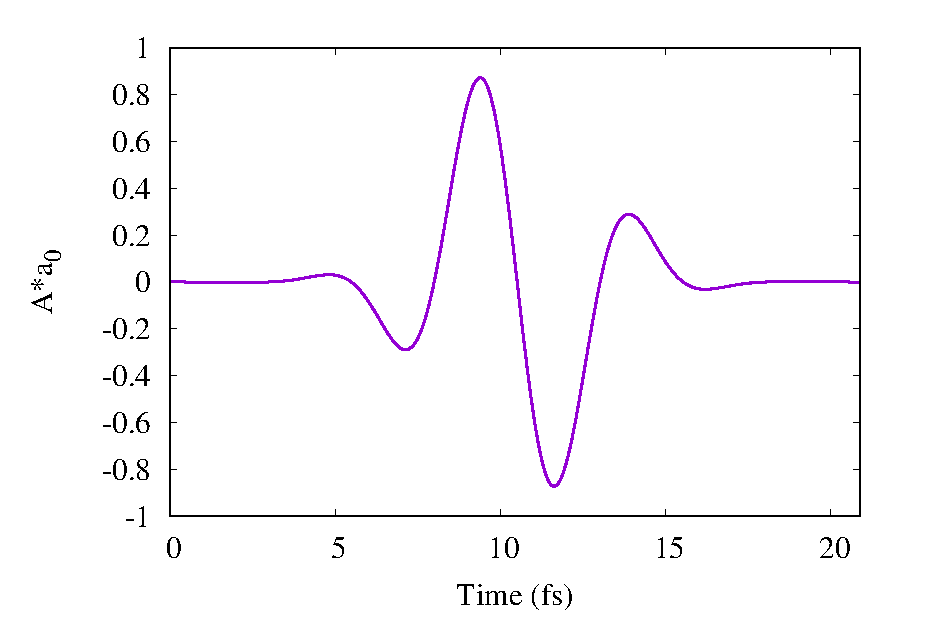
\includegraphics[width=1.0\linewidth,angle=0]{Pulse1p5A1.eps}
% \caption{The vector potential for the Gaussian pulse 
% with carrier $\omega=0.827$~eV, and $A_{0}\times a_0=1$.}
% \label{Pulse1p5A1}  
% \end{figure}

Our results are summarized in Figs.~4.2-4.4. 
Fig.~\ref{Fig:Light_induced_transition}a shows the electric field of the 
pulse carried at 1500 nm, while Fig.~\ref{Fig:Time_resolved_energy}b shows
the electric field of the pulse carried at 
3000 nm. The dynamical response is very similar in
these two cases.

Fig.~\ref{Fig:Light_induced_transition}(b-d) show the time-dependent population
densities [Eq.\eqref{Spectr_R_L_2} in Sec. \ref{subsection:Spectral_function} of \autoref{chap:Non_mb_th}] for increasing field
strength.  
Transfer of spectral weight from the van Hove singularity 
(located at the zero energy $E=0$) 
\begin{figure}[h!]
\begin{minipage}[h]{0.5\linewidth}
\center{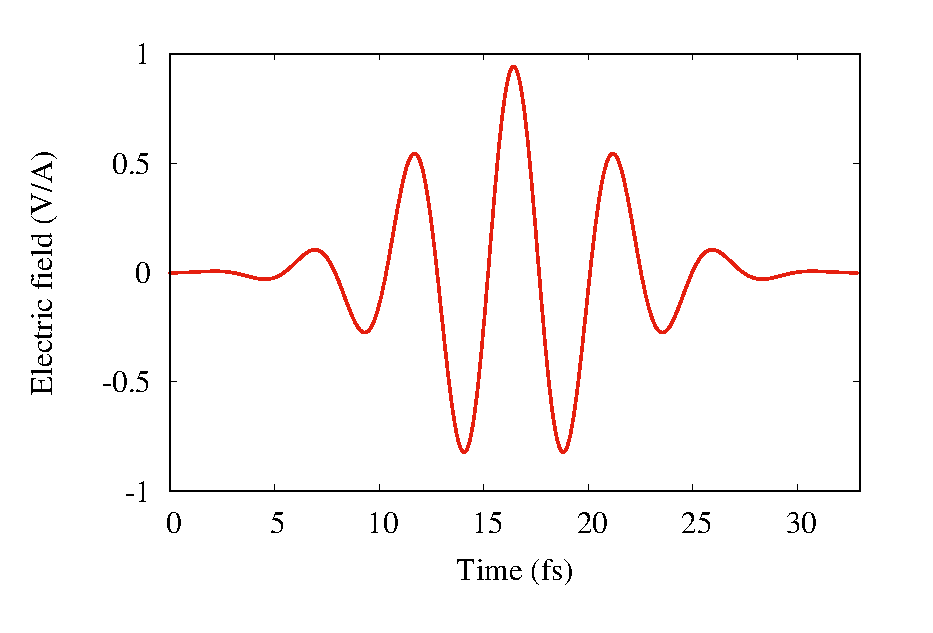
\includegraphics[width=1\linewidth]{Chapters/KH_solid/E_32.eps}} (a) \\
\end{minipage}
\hfill
\begin{minipage}[h]{0.5\linewidth}
\center{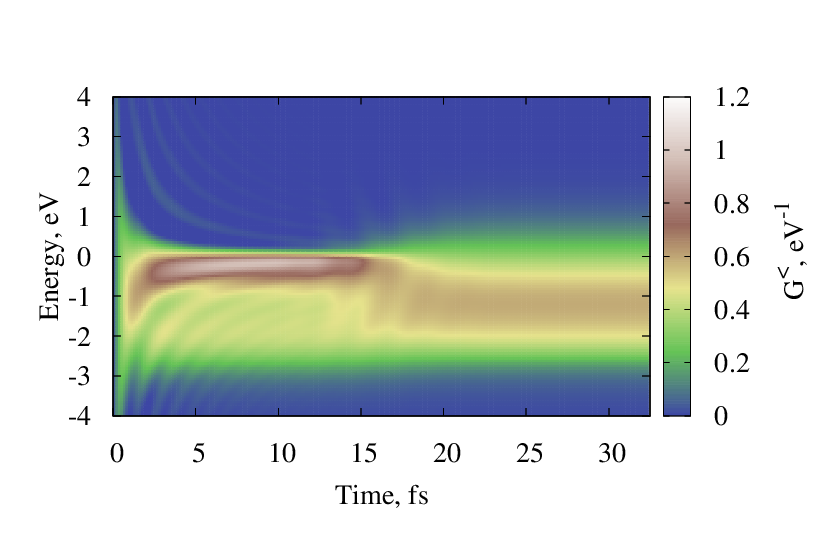
\includegraphics[width=1\linewidth]{Chapters/KH_solid/3d_les_E_1_10_9.png}} \\(b)
\end{minipage}
\begin{minipage}[h]{0.5\linewidth}
\center{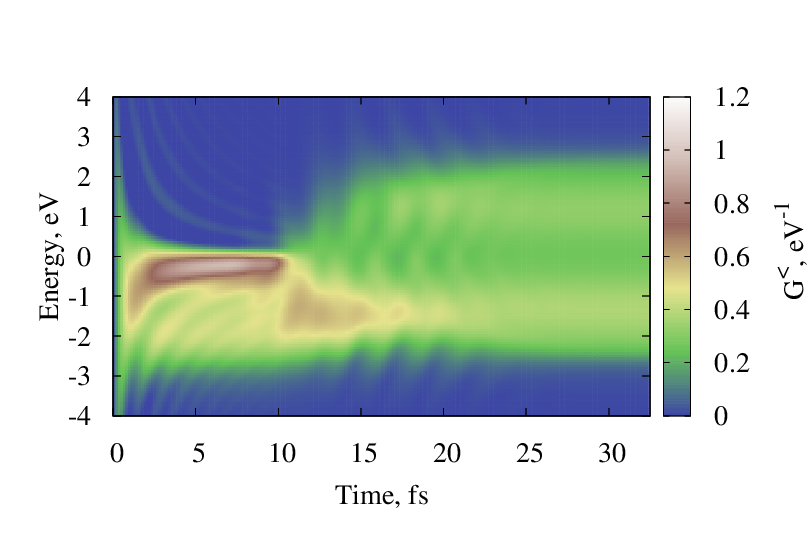
\includegraphics[width=1\linewidth]{Chapters/KH_solid/3d_les_E_5_10_9.png}} (c) \\
\end{minipage}
\hfill
\begin{minipage}[h]{0.5\linewidth}
\center{\includegraphics[width=1\linewidth]{Chapters/KH_solid/3d_les_E_2_10_10.png}} \\(d)
\end{minipage}
\caption{Light-induced transition from the metallic to 
the Mott-insulating state. 
(a) The electric field for the Gaussian pulse carried at 
$\omega=0.827$~eV used in the simulations. 
(b-d) Time-dependent population density for 
%$E_{max}=8*10^{8}$V/m (a),
the field amplitude $F_0=0.1$ V/A (b), 0.5 V/A (c), and 2.0 V/A (d).}
\label{Fig:Light_induced_transition}
\end{figure}
to the Hubbard bands becomes prominent 
as soon as the field approaches 0.1 V/A. 
The response is manifestly sub-cycle, within about 1 fs. 
At lower fields (Fig.~\ref{Fig:Light_induced_transition}b) the system stays predominantly in the lower Hubbard band during the whole interaction. 
It also does not return to the original distribution near the 
van Hove singularity once the pulse is over.
At higher fields (Fig.~\ref{Fig:Light_induced_transition}c), 
we see substantial population transfer from the lower 
to the upper Hubbard band (situated at $E=1.25$ eV) 
with the spectral gap opening. Blurring the graphs of occupied states within 5 femtoseconds is due to the lack of data for the Fourier transform from time to frequency.
The sub-cycle nature of the nonlinear response remains evident, 
including the splitting of the population between the upper and the lower bands as the electric field rapidly goes through its maxima, with the transient return of small spectral weight near zero energy as the electric field goes through zero. 
Crucially, the double-band Mott-type structure
survives well after the end of the pulse, 
Fig.~\ref{Fig:Light_induced_transition}(b-d), signifying 
the transition from a metallic to an insulating-type structure, 
induced by the laser field and stabilized by correlation.
The gap formation is confirmed by Fig.~\ref{Fig:Time_resolved_energy}, which shows that
the total energy in the system increases in steps synchronized with the instantaneous maxima in the laser electric field. 
This is true for both $\lambda=1500$ nm and $\lambda=3000$ nm
drivers. Note that the steps for both frequencies are
very similar in height, showing that the transitions are
in the quasi-static low-frequency regime.
\begin{figure}[h!]
\begin{minipage}[h]{0.5\linewidth}
\center{\includegraphics[width=1\linewidth]{Chapters/KH_solid/Etot_w192.eps}} (a) \\
\end{minipage}
\hfill
\begin{minipage}[h]{0.5\linewidth}
\center{\includegraphics[width=1\linewidth]{Chapters/KH_solid/Etot_w0961.eps}} (b) \\
\end{minipage}
\caption{Time-resolved energy absorption by the 
driven system with different peak field strengths (from $F_0=0.1$ V/A to $F_0=0.8$ V/A)
for 1500 nm (a) and 3000 nm (b). For guide we also show the shape of electric field.}
\label{Fig:Time_resolved_energy}
\end{figure}

Such frequency-independent step-wise behavior is characteristic of the tunneling limit in non-adiabatic excitation across a bandgap, be
it in an atom or a solid. In this regime the 
instantaneous transition amplitude across the 
energy gap is $A\propto \exp(-F_{\rm thr}/F(t))$. Here 
$F(t)$ is electric field with Gaussian envelop (Fig.~\ref{Fig:Light_induced_transition}a),
$F_{\rm thr}$ is the characteristic "threshold" field.
In a Mott insulator with a gap $\Delta$, 
$F_{\rm thr}\simeq \Delta /2\xi$ \cite{Oka_2003,Oka_2005,Oka_2010,Oka_2012}, where
$\xi\sim a_0$ is the correlation length. In our system,
an estimate for $F_{\rm thr}$ 
along the lattice direction is $F_{\rm thr}\sim U/2a_0=0.33 $V/A,
implying the threshold electric field amplitude of $F\simeq F_{\rm thr}\sqrt{2}=0.47$ V/A along the [11] direction. This estimate
is in excellent agreement with the observed behavior of 
$E_{\rm tot}(t)$, where the  
fields with amplitude $F>0.4-0.5$ V/A lead to 
saturation of excitation within a field cycle.
\begin{figure}[h!]
 \includegraphics[width=0.9\linewidth,angle=0]{Chapters/KH_solid/2_w_0_961.png}
\caption{Upper panel: A gaussian pulse at a central frequency $\omega=0.413$~eV, width $d=7.7$~fs, and intensity $F_{0}=0.8$~V/A, polarization along [11]. The generated current is shown in red. Middle panel: Time-dependent PES, dash lines denotes positions of Hubbard bands $\pm U/2$ (with $U=2.5$). Lower panel: Gabor transform of the current the dash line denotes position of odd $\omega$ harmonics generation in case of constant ac-field.}
\label{HHG_1}  
\end{figure}

As expected in the low-frequency regime, the
transition from the 
metallic phase to dynamical localization with
a gap is very similar for 3000 nm driver, and 
occurs as the instantaneous 
electric field exceeds $\sim 0.1-0.2$ V/A. An example
is shown in Fig.~\ref{HHG_1}, for the peak amplitude
of the driving field $F_{0}=0.8$ V/A.
Fig.~\ref{HHG_1}(upper panel) shows the driving electric field
(blue) and the generated current (red). Fig.~\ref{HHG_1}(middle panel) shows 
the time-resolved formation of the 
lower Hubbard band and the gap, as tracked by 
$I(\omega, t_p)$. In Fig.~\ref{HHG_1}(middle panel), the gap opens around 7-8 fs, 
when the instantaneous field reaches $\sim 0.1-0.2$ V/A. 
The excitations across the bandgap into the upper Hubbard 
band occur near the maxima of the instantaneous 
field, most notably at $\sim 12-13$ fs and $\sim 16-17$ fs.
Excitation is accompanied by 
suppression of the current, which is fully quenched 
at $\sim 18$ fs, when the excitation of the upper Hubbard band 
saturates and the insulating state is established. 
\begin{figure}[h!]
 \includegraphics[width=0.9\linewidth,angle=0]{Chapters/KH_solid/2_w_1_92.png}
\caption{Upper panel: A gaussian pulse at a central frequency $\omega=0.827$~eV, width $d=7.7$~fs, and intensity $F_{0}=0.8$~V/A, polarization along [11]. The generated current is shown in red. Middle panel: Time-dependent PES, dash lines denotes positions of Hubbard bands $\pm U/2$ (with $U=2.5$). Lower panel: Gabor transform of the current the dash line denotes position of odd $\omega$ harmonics generation in case of constant ac-field.}
\label{HHG_2}  
\end{figure}

The time-resolved optical signatures of charge dynamics are
encoded in the induced current and the 
coherent emission it generates (given 
by the Fourier transform of the current). As we have
already pointed out, time-resolved characterization of
the emission is feasible with about 1 fs accuracy.
The emergence of the gap and the step-wise injection of
charge across the gap inevitably lead to bursts
of current near the field maxima. Their Fourier transform
produces characteristic odd harmonics (dominated by
3rd and fifth), often referred to
as the Brunel harmonics \cite{Burnett_1989}. Thus, we expect that
efficient harmonic generation would start
with the formation of the Mott gap and cease when the excitation across the gap is saturated. 

The harmonics generation in Fig.~\ref{HHG_1} not coincide with odd frequencies of the pulse with limitation low-frequency external field by the Gaussian envelope. In Fig.~\ref{HHG_2} situation changing due to increasing the pulse frequency.


These expectations
are confirmed in Fig.~\ref{HHG_1}(bottom panel), which shows the FROG-type 
spectrogram of the emission, obtained using the Gabor transform
with a 3-fs (full width at half-maximum) Gaussian window. Indeed, the spectrogram contains clear information about the laser-induced reshaping of
the many-body state and the formation of the Mott gap. 
When the system is in the metallic state, the field
generates a strong current at the driving frequency. 
Harmonics are synchronized with the formation of
the gap and cease when light-induced step-wise transitions
across the bandgap are saturated. 



\section{Summary}

Modification of the electronic properties
of quantum systems with light opens new opportunities for
using light to tailor the ultrafast electronic response. 
Our work brings the strong-field concepts developed for
atomic systems in the context of strongly correlated
metals. 

%Altering the effective 
%potential for the electron motion with strong pulse light we 
%convert the system from a metallic state to the state
%with a Mott gap. 

We show how many-body correlations help to establish the field-induced transient insulator out of delocalized electrons. After the pulse, the system is transferred into a state of high electron temperature, which is inaccessible under equilibrium conditions and remains more insulating than the initial state, with a pseudo-gap. 
The dynamics in time-domain is 
resolved via harmonic generation spectroscopy, which 
encodes the formation of the Mott gap, 
excitation dynamics across it, and the establishment 
of the insulating state. 
Our findings demonstrate the possibility of manipulating phases 
of correlated systems with strong, non-resonant  
fields in a manner that is extremely robust with respect to the specific
frequency of the driving field, with the time-domain 
mechanisms opening a new regime of "beyond-Floquet" engineering of 
strongly correlated systems.

\FloatBarrier
\section{\label{beyond_Floquet}Appendix: Beyond-Floquet parametrization.}

To show the difference of regimes in current article calculations and high-frequency Floquet behavior we would like to demonstrate how much the dependence of the band narrowing on the magnitude of the vector potential. Here we use vector potential with [11] polarization limited by Gaussian envelope.  The mean value of the vector potential $\tilde{A}$ selected in the range from -FWHM to FWHM. Below we provide calculations for 2D square lattice with initial inverse temperature $\beta=1/T=5$ and $50 \times 50$ $k$-grid. For convenient comparison with other theoretical works all results in units of hopping. Where $t=1=0.43$eV; $U=5.81t=2.5$eV; $W=8t=3.44$eV; $\omega=1.92t=0.827$eV. 
\begin{figure}[h!]
\begin{minipage}[h]{0.5\linewidth}
\center{\includegraphics[width=1\linewidth]{Chapters/KH_solid/Intensity_of_LHB_occ_1.eps}} (a) \\
\end{minipage}
\hfill
\begin{minipage}[h]{0.5\linewidth}
\center{\includegraphics[width=1\linewidth]{Chapters/KH_solid/Width_of_LHB_occ_1.eps}} (b) \\
\end{minipage}
\caption{Dependence of intensity (a) and FWHM (b) of lower Hubbard band on the average value of vector potential $\tilde{A}$ in the middle of the pulse.}
\label{Fig:LHB_I_W}
\end{figure}

We consider two quantities: Intensity of lower Hubbard band(LHB) (Fig.~\ref{Fig:LHB_I_W}a) and FWHM (Fig.~\ref{Fig:LHB_I_W}b) of lower Hubbard band in the middle of the pulse where the value of vector potential equal zero. Both graphs were calculated using the photoemission spectrum and were also compared with data obtained from DOS.
\begin{figure}[h!]
\begin{minipage}[h]{0.5\linewidth}
\center{\includegraphics[width=1\linewidth]{Chapters/KH_solid/E_tot_1.eps}} (a) \\
\end{minipage}
\hfill
\begin{minipage}[h]{0.5\linewidth}
\center{\includegraphics[width=1\linewidth]{Chapters/KH_solid/docc_1.eps}} (b) \\
\end{minipage}
\caption{Dependence of total energy (a) and double occupancy (b) on the average value of vector potential $\tilde{A}$ in the middle of the pulse.}
\label{Fig:E_tot_docc_KH}
\end{figure}
The purple line corresponds to the position of zeros in zero-order Bessel function $J_0(A_x)$. One can expect that in the Floquet regime intensity of LHB will be maximum at positions of $J_0(\tilde{A}_x)=0$. For high-frequency regime ($\omega=10.47$ and $\omega=20.94$) the maximum of LHB achieve $J_0(\tilde{A}_x)=0$. For low pulse frequency, the intensity of LHB ceases to be consistent with the behavior of the $J_0(A_x)$.

Fig.~\ref{Fig:E_tot_docc_KH}a,b show dependence of total energy and double occupancy on the $\tilde{A}$ in the middle of the pulse. Energy absorption is significantly lager for low frequency ($\omega=1.92$ and $\omega=5.24$) as well as the number of excitations.


\FloatBarrier
\section{\label{Benchmark}Appendix: Benchmark of IPT results and exact diagonalization}

We performed a benchmark of our IPT on square lattice to the code 
Ref. \cite{Rui}, performing exact diagonalization for the finite 12-site one-dimensional chain.
\begin{figure}[h!]
 \includegraphics[width=0.9\linewidth,angle=0]{Chapters/KH_solid/HHGtestVitja.png}
\caption{Higher harmonic generation on square lattice for gaussian pulse with central frequency $\omega=10$~eV, $FWHM=3$~fs, and $A_{0}=5$, polarization along [10] direction. Upper panel: vector potential (blue) and current (green); middle panel: Gabor transform of the current; Lower panel: spectra of incoming pulse (blue) and current (green).}
\label{HHGtestVitja}  
\end{figure}
The hoppings $t=1$~eV, on-site Coulomb repulsion $U=6$~eV, pulse vector potential amplitude $A_{0}=5$, pulse FWHM is 3 fs, pulse central frequency $\omega=10$~eV. In order to compare our two-dimensional lattice model to one-dimensional chain, we choose linear pulse polarization along [10] direction and relatively large field amplitude.

Although the physics of 1D and 2D systems is different in sense of 
possibility of closed loops and additional scattering channels in two-dimensional lattice, the resulting HHG spectra are looking qualitatively similar (see Figs. \ref{HHGtestVitja} and \ref{HHGtestRui}).  
\begin{figure}[h!]
 \includegraphics[width=0.9\linewidth,angle=0]{Chapters/KH_solid/HHGtestRui.png}
\caption{Higher harmonic generation on 12-sites chain for gaussian pulse with central frequency $\omega=10$~eV, $FWHM=3$~fs, and $A_{0}=5$, polarization along the chain. Upper panel: vector potential (blue) and current (green); middle panel: Gabor transform of the current; Lower panel: spectra of incoming pulse (blue) and current (green, red, cyan).}
\label{HHGtestRui}  
\end{figure}
















%\tableofcontents
\chapter{Nonequilibrium-induced Lifshitz transitions}
\label{chap:FS}

\section{Introduction}
In this chapter, we introduce time-dependent light-induced engineering of the Fermi surface (FS) for materials with strong electronic correlations. 

An external electric field changes the band structure \cite{Principi_2016}, and as a result a change in the FS occurs. Such an electronic topological transition called Lifshitz transition.
We address nonequilibrium-induced Lifshitz transition caused by the applied external electric field in a case one-band Hubbard model on a 2D square lattice.

The Lifshitz transition can be also induced by doping, external pressure or external magnetic field and has been experimentally observed in many real systems, such as heavy-fermion systems 
\cite{PhysRevB.86.075108, PhysRevLett.110.256403, PhysRevLett.116.037202}, 
iron-based superconductors \cite{PhysRevB.83.020501, PhysRevB.86.165117, PhysRevB.88.220508, PhysRevLett.112.156401, PhysRevB.90.224508, Liu_2010_FS}, 
cuprate high-temperature superconductors \cite{PhysRevB.81.180513, PhysRevB.83.054506, PhysRevLett.114.147001, PhysRevLett.120.067002, PhysRevB.81.121102}.


%\FloatBarrier


%\section{\label{Theory} Model and method}

We take the single-band Hubbard model driven by an electric field with the Hamiltonian:
\begin{equation}
\begin{split}
H(t)&=\sum_{ij,\sigma}t_{ij}{\rm exp}{\left( -i\int_{{\bf R}_{j}}^{{\bf R}_{i}}d{\bf r} \cdot {\bf A}(t) \right)}c_{i \sigma}^{\dagger}c_{j \sigma}\\
&+\mu {\sum_{i,\sigma} n_{i \sigma}}+U{\sum_{i} n_{i \uparrow}n_{i \downarrow}},
\end{split}
\end{equation}
where $t_{ij}$ is electron hopping amplitudes between sites $i$ and $j$, $U$ is the on-site Coulomb interaction, $c_{i \sigma}^{\dagger}$ creates an electron at site $i$ and spin $\sigma$, and 
$n_{i\sigma}=c_{i\sigma}^{\dagger}c_{i\sigma}$ is the number operator. We incorporate the effect of 
an external electric field ${\bf E(t)} = -\partial{\bf A}(t)/\partial t$ in terms of the Peierls
substitution \cite{Peierls1933} for the vector potential ${\bf A}$ into the hopping \cite{PhysRevLett.106.236401, PhysRevB.91.245153}.  

Exploiting this property, we can direct the electric field along one of the crystallographic axes, which gives a quasi-one-dimensional model, 
or along the diagonal of the square lattice, which gives physics similar to the hypercubic lattices but with the 2D band structure that includes the van Hove singularity.

In order to treat the time-dependent problem, we use non-equilibrium IPT which was discussed in Sec. \ref{subsection:Impurity_solvers} of \autoref{chap:Non_mb_th} in detail.

We consider the square lattice with the band dispersion,
\begin{equation}
\begin{split}
 \varepsilon({\bf k},t)&=2t\left[{\rm cos}(k_x+A_x(t))+
{\rm cos}(k_y+A_y(t))\right]\\
 &+4t'{\rm cos}(k_x+A_x(t)) {\rm cos}(k_y+A_y(t)),
 %\\
 % &{ { +2t_3(cos(2k_x+2{\bf A}_x(t))+cos(2k_y+2{\bf A}_y(t)))}}.
\end{split}
\label{dispersion}
\end{equation}
where $t=1$ is the nearest-neighbor (NN) and $t'=-0.32$ is next nearest-neighbor (NNN) hopping amplitude. 
Time has units of reverse hoppings. 
DMFT based retarded and lesser Green's functions can give information about excitation and occupation spectrum Eq. \eqref{Spectr_R_L_1},\eqref{Spectr_R_L_2} in Sec. \ref{subsection:Spectral_function} of \autoref{chap:Non_mb_th}. The $k$-resolved spectral function and occupied density of states diven by Eq. \eqref{Spectr_R_L_k_1},\eqref{Spectr_R_L_k_2} in Sec. \ref{subsection:Spectral_function} of \autoref{chap:Non_mb_th}.
The shape of the vector potential is depicted in Fig.~\ref{fig:A_shape_FS}.
\begin{figure}[h!]
%\begin{minipage}[h]{0.51\linewidth}
\center{\includegraphics[width=0.6\linewidth]{Chapters/Fermi_surface/figures/Pulse_shape.eps}} \\
%\end{minipage}
\caption{Shape of vector potential ($\omega=21$, $t_0=6.85$).}
\label{fig:A_shape_FS}
\end{figure}
and is expressed by the formula:
\begin{equation}
%A(t)={A_{\rm max}{\rm exp}\left[-\frac{(t-t_0)}{2\sigma ^2}]}sin[\omega(t-t_0)+\phi+\frac{r_c t^2}{2}\right],
A(t)={A_{\rm max}{\rm exp}\left[-\frac{(t-t_0)^2}{2\sigma ^2}\right]}sin(\omega(t-t_0)),
\label{Ashape}
\end{equation}
where parameters are:
$\sigma=\frac{d}{2\sqrt{2ln2}}$; pulse duration with $d$; full-width at half-maximum (FWHM);
amplitude of the vector potential $A_{\rm max}$;
frequency of the vector potential $\omega$;
peak time of the pulse $t_0$.
Below we provide calculations for $\beta=5$ and $32 \times 32$ $k$-grid. 

%%%%%%%%%%%%%%%%%%%%%%%%%%%%%%%%%%%%%%%%%%%%%%%%%%%%%%%%%%%%%%%%%%
\FloatBarrier

\section{Case of the NN-hopping}

\subsection{FS parameters selection}

Calculating the FS we have to move from $k$-independent local quantities to $k$-resolved. In the first part of the chapter, we consider a square lattice with the nearest neighbors hopping whose FS is represented by a dashed line in the Fig.~\ref{fig:BZ_sq_lat}.
\begin{figure}[h!]
%\begin{minipage}[h]{0.51\linewidth}
\center{\includegraphics[width=0.35\linewidth]{Chapters/Fermi_surface/figures/square_lattice/BZ_1.pdf}} \\
%\end{minipage}
\caption{Brillouin zone for a square lattice}
\label{fig:BZ_sq_lat}
\end{figure}
Using the Green's functions on the Keldysh contour for a finite-dimensional lattice is computationally expensive and heavily limits the time of the simulations. In this chapter, we focus on transient dynamics and states immediately after the pulse. 
\begin{figure}[h!]
\begin{minipage}[h]{0.5\linewidth}
\center{\includegraphics[width=1\linewidth]{Chapters/Fermi_surface/figures/square_lattice/xy/G_l_loc.png}} (a) \\
\end{minipage}
\hfill
\begin{minipage}[h]{0.5\linewidth}
\center{\includegraphics[width=1\linewidth]{Chapters/Fermi_surface/figures/square_lattice/y/1_75/G_l_loc.png}} (b) \\
\end{minipage}
\caption{Local $G^{<}(t,t')$ for $A_{max}=1.75$ and $U=6$ with different polarizations of vector potential: (a) $XY$- polarization; (b) $Y$-polarization.}
\label{fig:G_loc_3d}
\end{figure}
Also, we define the model parameters to be the most suitable for the FS interpretation.

In the presence of a particle-hole symmetry, the challenge is to achieve a decay of the Green's functions inside considered simulation time.
In the case of local Green's functions, the damping occurs rather quickly for all considered polarizations of the external field (Fig.~\ref{fig:G_loc_3d}). Such attenuation in time will give a quantitatively correct result for the frequency dependence quantities obtained via Fourier transform. 
\begin{figure}[h!]
\begin{minipage}[h]{0.5\linewidth}
\center{\includegraphics[width=1\linewidth]{Chapters/Fermi_surface/figures/square_lattice/Gret_xy_mid_Y_u.eps}} (a) \\
\end{minipage}
\hfill
\begin{minipage}[h]{0.5\linewidth}
\center{\includegraphics[width=1\linewidth]{Chapters/Fermi_surface/figures/square_lattice/Gret_xy_mid_M_2_u.eps}} (b) \\
\end{minipage}
\caption{$G^{R}(t,t-s)_k$ ($time=6.85$) with different $U$ values for $A_{max}=1.5$ and $XY$-polarization: (a) Y-point of BZ; (b) M/2-point of BZ.}
\label{fig:G_k_res_ret_u_dep}
\end{figure}

In the case of $k$-resolved Green's functions, the damping is much slower for particular $k$-points. In Fig.~\ref{fig:G_k_res_ret_u_dep} the dependence of the Green's function on time for different $U$ is shown for Y and M/2-points in the Brillouin zone (BZ). 
\begin{figure}[h!]
\begin{minipage}[h]{0.5\linewidth}
\center{\includegraphics[width=1\linewidth]{Chapters/Fermi_surface/figures/square_lattice/Gret_xy_mid_Y.eps}} (a) \\
\end{minipage}
\hfill
\begin{minipage}[h]{0.5\linewidth}
\center{\includegraphics[width=1\linewidth]{Chapters/Fermi_surface/figures/square_lattice/Gret_xy_mid_M_2.eps}} (b) \\
\end{minipage}
\caption{$G^{R}(t,t-s)_k$ ($time=6.85$) with different $A_{max}$ values for $U=6$ and $XY$-polarization : (a) Y-point of BZ; (b) M/2-point of BZ.}
\label{fig:G_k_res_ret_A_dep_xy}
\end{figure}
Increasing Coulomb interaction the dumping of the Green's function becomes stronger. These highly symmetrical points were chosen due to the fact that they belong to the FS and have the highest intensity of the spectral function at a frequency equal to zero and the smallest attenuation of the corresponding two-time Green's function. 

In the Fig.~\ref{fig:G_k_res_ret_A_dep_xy} the dependence of the Green's function on time for different values of vector potential for $XY$-polarization of vector potential is shown. An increase of the vector potential leads to a faster decay of the Green's function. 
\begin{figure}[ht]
\begin{minipage}[h]{0.5\linewidth}
\center{\includegraphics[width=1\linewidth]{Chapters/Fermi_surface/figures/square_lattice/DOS_xy_mid_Y.eps}} (a) \\
\end{minipage}
\hfill
\begin{minipage}[h]{0.5\linewidth}
\center{\includegraphics[width=1\linewidth]{Chapters/Fermi_surface/figures/square_lattice/OCC_xy_mid_Y.eps}} (b) \\
\end{minipage}
\caption{Spectrum of the full number of states $A^{R}(t=6.85,\omega)_{k=\text{Y}}$ (a) and occupied states $A^{<}(t=6.85,\omega)_{k=\text{Y}}$ (b) with different $A_{max}$ values for $U=6$ and $XY$-polarization.}
\label{fig:G_k_res_ret_A_dep_w_xy}
\end{figure}

The corresponding spectral functions are shown in the Fig.~\ref{fig:G_k_res_ret_A_dep_w_xy}. Some of them have negative values \citep{PhysRevB.71.085104,PhysRevB.73.209902,PhysRevB.80.115119,PhysRevLett.112.176404} that partially appear as a result of the particular form of the Fourier transform used on the work.
\begin{figure}[ht]
\begin{minipage}[h]{0.5\linewidth}
\center{\includegraphics[width=1\linewidth]{Chapters/Fermi_surface/figures/square_lattice/Gret_y_mid_Y.eps}} (a) \\
\end{minipage}
\hfill
\begin{minipage}[h]{0.5\linewidth}
\center{\includegraphics[width=1\linewidth]{Chapters/Fermi_surface/figures/square_lattice/Gret_y_mid_M_2.eps}} (b) \\
\end{minipage}
\caption{$G^{R}(t,t-s)_k$ ($time=6.85$) with different $A_{max}$ values for $U=6$ and $Y$-polarization: (a) Y-point of BZ; (b) M/2-point of BZ.}
\label{fig:G_k_res_ret_A_dep_y}
\end{figure}

As can be seen from Fig.~\ref{fig:G_k_res_ret_A_dep_y}, similar dependence of the attenuation of the Green's functions on the magnitude of the vector potential takes place for the case of $Y$-polarization.
Also, similar to the $XY$-polarization case, $Y$-polarized pulse transfers states (Fig.~\ref{fig:G_k_res_ret_A_dep_w_y}a) and particles (Fig.~\ref{fig:G_k_res_ret_A_dep_w_y}b) from the low-frequency to the high-frequency region.
\begin{figure}[h!]
\begin{minipage}[h]{0.5\linewidth}
\center{\includegraphics[width=1\linewidth]{Chapters/Fermi_surface/figures/square_lattice/DOS_y_mid_Y.eps}} (a) \\
\end{minipage}
\hfill
\begin{minipage}[h]{0.5\linewidth}
\center{\includegraphics[width=1\linewidth]{Chapters/Fermi_surface/figures/square_lattice/OCC_y_mid_Y.eps}} (b) \\
\end{minipage}
\caption{Spectra of full number of states $A^{R}(t=6.85,\omega)_{k= \text{Y}}$ (a) and occupied states $A^{<}(t=6.85,\omega)_{k= \text{Y}}$ (b) for different $A_{max}$ values with $U=6$ and $Y$-polarization.}
\label{fig:G_k_res_ret_A_dep_w_y}
\end{figure}

In order to understand how the redistribution of electrons occurs due to increasing of the magnitude and direction of the pulse, we consider the local lesser Green's functions (Fig.~\ref{fig:G_loc_les_A_dep_w}). For all pulse polarizations, the maximum pumping of the Hubbard bands occurs in the region around the maximum of the pulse ($time=6.85$) due to the transfer of electrons to higher energy regions at $U/2$.
The higher the value of the vector potential becomes stronger the intensity of the Hubbard band and less in the low-frequency region for the $Y$-the direction of the vector potential (Figs.~\ref{fig:G_loc_les_A_dep_w}b,d,f). In the case of $XY$-polarization, the electron population of the low-frequency region can oscillate depending on the renormalized hopping value in accordance with the zero-order Bessel function \cite{PhysRevLett.106.236401}. The van Hove singularity nearly disappears in the pulse maximum at the $A_{max}=3.0$ for all polarizations.
Thus, for these parameters of the system, it is prudent to use a $A_{max}=1.75$ in which the convergence of the two-time Green's function is good and at the same time, there is a high density of states at the Fermi level during the pulse.
\begin{figure}[h!]
\begin{minipage}[h]{0.5\linewidth}
\center{\includegraphics[width=1\linewidth]{Chapters/Fermi_surface/figures/square_lattice/1_5_xy.png}} (a) \\
\end{minipage}
\hfill
\begin{minipage}[h]{0.5\linewidth}
\center{\includegraphics[width=1\linewidth]{Chapters/Fermi_surface/figures/square_lattice/1_5_y.png}} (b) \\
\end{minipage}
\begin{minipage}[h]{0.5\linewidth}
\center{\includegraphics[width=1\linewidth]{Chapters/Fermi_surface/figures/square_lattice/1_75_xy.png}} (c) \\
\end{minipage}
\hfill
\begin{minipage}[h]{0.5\linewidth}
\center{\includegraphics[width=1\linewidth]{Chapters/Fermi_surface/figures/square_lattice/1_75_y.png}} (d) \\
\end{minipage}
\begin{minipage}[h]{0.5\linewidth}
\center{\includegraphics[width=1\linewidth]{Chapters/Fermi_surface/figures/square_lattice/3_0_xy.png}} (e) \\
\end{minipage}
\hfill
\begin{minipage}[h]{0.5\linewidth}
\center{\includegraphics[width=1\linewidth]{Chapters/Fermi_surface/figures/square_lattice/3_0_y.png}} (f) \\
\end{minipage}
\caption{Occupied states $A^{<}(t,\omega)$ for $U=6$: (a) $A_{max}=1.5$ $XY$-polarization; (b) $A_{max}=1.5$ $Y$-polarization; (c) $A_{max}=1.75$ $XY$-polarization; (d) $A_{max}=1.75$ $Y$-polarization; (e) $A_{max}=3.0$ $XY$-polarization; (f) $A_{max}=3.0$ $Y$-polarization.}
\label{fig:G_loc_les_A_dep_w}
\end{figure}

It is worth noting the behavior of the peak at low frequency for the $XY$ pulse polarization. For all considered values of the $A_{max}$ the number of electrons and states at the Fermi level increases during the second half of the pulse (Figs.~\ref{fig:G_loc_les_A_dep_w0} and \ref{fig:G_loc_les_A_dep_w}a,b,c,d). For the $XY$-polarization the intensity becomes even greater than it was in the equilibrium case before pulse (Fig.~\ref{fig:G_loc_les_A_dep_w0}a) for values of $A_{max}<2.0$.
\begin{figure}[h!]
\begin{minipage}[h]{0.5\linewidth}
\begin{overpic}[width=1\textwidth]{Chapters/Fermi_surface/figures/square_lattice/xy/sum_QP_xy.eps}
 \put (22,56) {(a)}
\end{overpic}
\end{minipage}
\hfill
\begin{minipage}[h]{0.5\linewidth}
\begin{overpic}[width=1\textwidth]{Chapters/Fermi_surface/figures/square_lattice/y/sum_QP.eps}
 \put (22,56) {(b)}
\end{overpic}
\end{minipage}
\caption{The intensity of the occupied states at zero frequency $A^{<}(t,\omega=0)$ (a) $XY$-polarization; (b) $Y$-polarization.}
\label{fig:G_loc_les_A_dep_w0}
\end{figure}

\begin{figure}[h!]
\begin{minipage}[h]{0.5\linewidth}
\begin{overpic}[width=1\textwidth]{Chapters/Fermi_surface/figures/square_lattice/y/1_75/G_l_k_M.png}
 \put (16,60) {\textcolor{white}{(a)}}
\end{overpic}
\end{minipage}
\hfill
\begin{minipage}[h]{0.5\linewidth}
\begin{overpic}[width=1\textwidth]{Chapters/Fermi_surface/figures/square_lattice/y/1_75/G_l_k_Y.png}
 \put (16,60) {\textcolor{white}{(b)}}
\end{overpic}
\end{minipage}
\begin{minipage}[h]{0.5\linewidth}
\begin{overpic}[width=1\textwidth]{Chapters/Fermi_surface/figures/square_lattice/y/1_75/G_l_k_M_2.png}
 \put (16,60) {\textcolor{white}{(c)}}
\end{overpic}
\end{minipage}
\hfill
\begin{minipage}[h]{0.5\linewidth}
\begin{overpic}[width=1\textwidth]{Chapters/Fermi_surface/figures/square_lattice/y/1_75/G_l_k_X.png}
 \put (16,60) {\textcolor{white}{(d)}}
\end{overpic}
\end{minipage}
\caption{$G^{<}(t,t')_k$ for $A_{max}=1.75$, $U=6$, $Y$ - pulse polarization and different $k$-points of BZ: (a) M; (b) Y; (c) M/2; (d) X.}
\label{fig:G_k_3d_square_latt}
\end{figure}

After choosing the optimal lattice and pulse parameters, we have to make sure that the $A^{<}(t,\omega)_k$ decays within the simulation time. 
Fig.~\ref{fig:G_k_3d_square_latt} shows the values of the two-time Green's function for various points of the Brillouin zone for the optimal parameters. Starting from $time=6$ the Green's functions decays to nearly zero values rather quickly, giving the correct results after Fourier transforms in the frequency domain.
\begin{figure}[h!]
\begin{minipage}[h]{0.5\linewidth}
\begin{overpic}[width=1\textwidth]{Chapters/Fermi_surface/figures/square_lattice/xy/band_eq/Band_r_time_1370.png}
 \put (16,60) {\textcolor{white}{(a)}}
\end{overpic}
\end{minipage}
\hfill
\begin{minipage}[h]{0.5\linewidth}
\begin{overpic}[width=1\textwidth]{Chapters/Fermi_surface/figures/square_lattice/xy/band_eq/Band_l_time_1370_0.png}
 \put (16,60) {\textcolor{white}{(b)}}
\end{overpic}
\end{minipage}
\caption{Equilibrium band structure (a) and occupied states (b).}
\label{fig:Eq_band_occ_u6}
\end{figure}

Consider how the band structure and occupied states change under the influence of the external field. 
Fig.~\ref{fig:Eq_band_occ_u6} shows the equilibrium band structure and occupied states at the high-symmetry points of the first Brillouin zone. 
\begin{figure}[h!]
\begin{minipage}[h]{0.5\linewidth}
\begin{overpic}[width=1\textwidth]{Chapters/Fermi_surface/figures/square_lattice/xy/Band_r_time_1370.png}
 \put (16,60) {\textcolor{white}{(a)}}
\end{overpic}
\end{minipage}
\hfill
\begin{minipage}[h]{0.5\linewidth}
\begin{overpic}[width=1\textwidth]{Chapters/Fermi_surface/figures/square_lattice/xy/Band_l_time_1370_0.png}
 \put (16,60) {\textcolor{white}{(b)}}
\end{overpic}
\end{minipage}
\caption{Band structure (a) and occupied states (b) in the middle of pulse for $A_{max}=1.75$ and $XY$ - pulse polarization.}
\label{fig:band_occ_A_1_75_xy}
\end{figure}

The maximum intensity at the Fermi level is caused by the presence of a van Hove due to the geometry of the system. 
The blurring that distinguishes this electronic structure from tight-binding is caused by the large influence of the electronic correlations.

Under the influence of an external electric field in the $XY$-polarization a redistribution of states occurs.
The spectral weight from the van Hove singularity goes symmetrically to the energy regions $-U/2$ and $U/2$ (Fig.~\ref{fig:band_occ_A_1_75_xy}a). Since the pulse frequency is significantly higher than the bandwidth, the electronic structure is rearranged to be more correlated with almost no electron transfer beyond the Fermi level (energy absorption for high-frequency pulse discussed in Sec.~\ref{E_A}).
The last statement can be observed on the density of occupied states (Fig.~\ref{fig:band_occ_A_1_75_xy}b) that stays below the Fermi level during a pulse. 
\begin{figure}[h!]
\begin{minipage}[h]{0.5\linewidth}
\begin{overpic}[width=1\textwidth]{Chapters/Fermi_surface/figures/square_lattice/y/1_75/Band_r_time_1370.png}
 \put (16,60) {\textcolor{white}{(a)}}
\end{overpic}
\end{minipage}
\hfill
\begin{minipage}[h]{0.5\linewidth}
\begin{overpic}[width=1\textwidth]{Chapters/Fermi_surface/figures/square_lattice/y/1_75/Band_l_time_1370_0.png}
 \put (16,60) {\textcolor{white}{(b)}}
\end{overpic}
\end{minipage}
\begin{minipage}[h]{0.5\linewidth}
\begin{overpic}[width=1\textwidth]{Chapters/Fermi_surface/figures/square_lattice/y/3_0/Band_r_time_1370.png}
 \put (16,60) {\textcolor{white}{(c)}}
\end{overpic}
\end{minipage}
\hfill
\begin{minipage}[h]{0.5\linewidth}
\begin{overpic}[width=1\textwidth]{Chapters/Fermi_surface/figures/square_lattice/y/3_0/Band_l_time_1370_0.png}
 \put (16,60) {\textcolor{white}{(d)}}
\end{overpic}
\end{minipage}
\caption{(a) Band structure $A_{max}=1.75$; (b) occupied states $A_{max}=1.75$; (c) band structure $A_{max}=3.0$; (d) occupied states $A_{max}=3.0$ in the middle of pulse for $Y$- pulse polarization.}
\label{fig:band_occ_A_1_75_and_3_0_y}
\end{figure}

In the case of the $Y$-polarization of the field, the Hubbard bands are also get populated (Fig.~\ref{fig:band_occ_A_1_75_and_3_0_y}a), but they are not as localized in energy as in case of $XY$-polarization. Due to the influence of the $Y$-polarization, some points in BZ become no longer equivalent. The symmetry breaks for [11] direction. The FS portion gets a bend as can be seen in Fig.~\ref{fig:band_occ_A_1_75_and_3_0_y}a,b along Y to X path.
With an increase in the vector potential to $A_{max}=3.0$ the number of states at $\omega=0$ 
decays since they are moving to higher energies than $-U/2$ and $U/2$.

It should be noted that all time-dependent band structures are built at the $time=6.85$ when the Gaussian envelope has maximum (the middle of the pulse) and the value of the oscillating vector potential is equal to zero.

\FloatBarrier


\subsection{Lifshitz transitions (NN - hopping)}

Although the nonequilibrium distribution function during the pulse substantially differs from the Fermi-Dirac one, 
we can still keep track of the FS. 
\begin{figure}[h!]
\begin{minipage}[h]{0.5\linewidth}
\center{\includegraphics[width=1\linewidth]{Chapters/Fermi_surface/figures/square_lattice/xy/band_eq/FS_time_1370.eps}} (a) \\
\end{minipage}
\hfill
\begin{minipage}[h]{0.5\linewidth}
\center{\includegraphics[width=1\linewidth]{Chapters/Fermi_surface/figures/square_lattice/y/1_75/FS_time_1370_mid.eps}} (b) \\
\end{minipage}
\begin{minipage}[h]{0.5\linewidth}
\center{\includegraphics[width=1\linewidth]{Chapters/Fermi_surface/figures/square_lattice/y/1_75/FS_time_1370_md.eps}} (c) \\
\end{minipage}
\hfill
\begin{minipage}[h]{0.5\linewidth}
\center{\includegraphics[width=1\linewidth]{Chapters/Fermi_surface/figures/square_lattice/y/3_0/FS_time_1370.eps}} (d) \\
\end{minipage}
\caption{FS for $Y$-pulse polarization: (a) equilibrium; (b) $A_{max}=1.75$ in the middle of the pulse ($time=6.85$); (c) $A_{max}=1.75$ after the pulse ($time=13.7$); (d) $A_{max}=3.0$ in the middle of the pulse.}
\label{fig:FS_sq_latt_Y_field}
\end{figure}
In order to do so, we can introduce an extended definition of FS for out-of-equilibrium situations. 

Since our aim is a study of the evolution of initial FS, we focus on the electron density at the energy equal to equilibrium chemical potential. We have a direct access to this quantity via the Green's function $ImG^{<}(t,\omega)_k$ (see \autoref{chap:Non_mb_th} Eq. \ref{Spectr_R_L_k_2}).
 
The Fig.~\ref{fig:FS_sq_latt_Y_field} shows FS for $Y$-polarization. In the equilibrium case, the maximum intensities are distributed evenly as shown in the Fig.~\ref{fig:FS_sq_latt_Y_field}a. 
The action of the field renormalizes the intensity, thereby changing the structure. 
The maximum intensity is collected near the Y point and decreases significantly at the X point (Fig.~\ref{fig:FS_sq_latt_Y_field}b) as shown on the occupied band structure in Fig.~\ref{fig:band_occ_A_1_75_and_3_0_y}b. 

Like time-dependent band structures, FS are built at the time when the Gaussian envelope has maximum, and the value of the vector potential is equal to zero.

Qualitatively similar behavior has been observed for the 
Floquet stationary states Fig.~\ref{fig:FS_equilibrium_sq_latt_Y_field} (the calculation method will be discussed in more detail in the next part of the chapter). 
After the external field is turned off, the FS restores its original shape with a lower intensity (Fig.~\ref{fig:FS_sq_latt_Y_field}c). 
The destruction of the FS in time of a pulse is possible when a sufficiently large vector potential is applied (Fig.~\ref{fig:FS_sq_latt_Y_field}d).



\begin{figure}[h!]
%\begin{minipage}[h]{0.51\linewidth}
\center{\includegraphics[width=0.55\linewidth]{Chapters/Fermi_surface/figures/square_lattice/y/1_75/FS_time_1370_st_st.eps}} \\
%\end{minipage}
\caption{Equilibrium FS with renormalized hopping according to $A_{max}=1.75$ and $Y$ pulse polarization.}
\label{fig:FS_equilibrium_sq_latt_Y_field}
\end{figure}

The application of the field in the $XY$-polarization does not lead to a substantial rearrangement of the FS.
There is a transfer of intensity from the diagonal -Y-X to YX depending on the direction of the vector potential (Fig.~\ref{fig:FS_sq_latt_XY_field}a). After the pulse (Fig.~\ref{fig:FS_sq_latt_XY_field}b), by analogy with $Y$-polarization, a decrease in intensity is observed.
\begin{figure}[h!]
\begin{minipage}[h]{0.5\linewidth}
\center{\includegraphics[width=1\linewidth]{Chapters/Fermi_surface/figures/square_lattice/xy/FS_time_1370_mid.eps}} (a) \\
\end{minipage}
\hfill
\begin{minipage}[h]{0.5\linewidth}
\center{\includegraphics[width=1\linewidth]{Chapters/Fermi_surface/figures/square_lattice/xy/FS_time_1370_md.eps}} (b) \\
\end{minipage}
\caption{FS for $XY$ pulse polarization and $A_{max}=1.75$: (a) in the middle of the pulse ($time=6.85$); (b) after the pulse ($time=13.7$).}
\label{fig:FS_sq_latt_XY_field}
\end{figure}

%The temperature dependence on the value of total energy for the considered system is shown in Fig. \ref{fig:temperature_sqlat_u6}. 
%\begin{figure}[h!]
%\begin{minipage}[h]{0.51\linewidth}
%\center{\includegraphics[width=0.5\linewidth]{Chapters/Fermi_surface/figures/square_lattice/E_b_sq_latt.eps}} \\
%\end{minipage}
%\caption{The temperature dependence of the total energy.}
%\label{fig:temperature_sqlat_u6}
%\end{figure}


\FloatBarrier

\section{Case of the NNN-hopping}

\subsection{FS parameters selection}
In this chapter we consider a square lattice (Eq.~\ref{dispersion}) with the presence of the next neighbors hopping $t'=-0.32$. Adding next neighbor hopping we leave the partial-hole symmetry what leads to non-conservation of the number of particles during the pulse. The Fig.~\ref{fig:Particle_conservation_t_tp} shows the filling $n$ for various values vector potential $A_{max}$, and polarization.
In general, the number of particles in the system is better preserved at small vector potentials and in the middle of the pulse have more or less satisfactory values. In the following, we consider the properties of the system for $A_{max}=1.75$.
\begin{figure}[h!]
\begin{minipage}[h]{0.5\linewidth}
\center{\includegraphics[width=1\linewidth]{Chapters/Fermi_surface/figures/t_t_lattice/xy/n_xy_05.eps}} (a) \\
\end{minipage}
\hfill
\begin{minipage}[h]{0.5\linewidth}
\center{\includegraphics[width=1\linewidth]{Chapters/Fermi_surface/figures/t_t_lattice/xy/n_xy_0425.eps}} (b) \\
\end{minipage}
\begin{minipage}[h]{0.5\linewidth}
\center{\includegraphics[width=1\linewidth]{Chapters/Fermi_surface/figures/t_t_lattice/y/n_y_05.eps}} (c) \\
\end{minipage}
\hfill
\begin{minipage}[h]{0.5\linewidth}
\center{\includegraphics[width=1\linewidth]{Chapters/Fermi_surface/figures/t_t_lattice/y/n_y_0425.eps}} (d) \\
\end{minipage}
\caption{Particle conservation: (a) $n=0.5$ $XY$-polarization; (b) $n=0.425$ $XY$-polarization; (c) $n=0.5$ $Y$-polarization; (d) $n=0.425$ $Y$-polarization.}
\label{fig:Particle_conservation_t_tp}
\end{figure}

In the Fig.~\ref{fig:G_ret_t_tp}a is depicted local retarded Green's function oscillations of which damping very quickly. But the same $k$-resolved function decays much more slowly as it is shown in Fig.~\ref{fig:G_ret_t_tp}b.
\begin{figure}[h!]
\begin{minipage}[h]{0.5\linewidth}
\begin{overpic}[width=1\textwidth]{Chapters/Fermi_surface/figures/t_t_lattice/Gret_xy_mid_loc.eps}
 \put (83,55) {(a)}
\end{overpic}
\end{minipage}
\hfill
\begin{minipage}[h]{0.5\linewidth}
\begin{overpic}[width=1\textwidth]{Chapters/Fermi_surface/figures/t_t_lattice/Gret_xy_mid.eps}
 \put (83,55) {(b)}
\end{overpic}
\end{minipage}
\caption{$G^{R}(t,t-s)_k$ in the middle of the pulse for $A_{max}=1.75$: (a) local; (b) in Y-point of BZ.}
\label{fig:G_ret_t_tp}
\end{figure}

\begin{figure}[h!]
\begin{minipage}[h]{0.5\linewidth}
\begin{overpic}[width=1\textwidth]{Chapters/Fermi_surface/figures/t_t_lattice/xy/1_75/G_l_k_Y_05.png}
 \put (16,60) {\textcolor{white}{(a)}}
\end{overpic}
\end{minipage}
\hfill
\begin{minipage}[h]{0.5\linewidth}
\begin{overpic}[width=1\textwidth]{Chapters/Fermi_surface/figures/t_t_lattice/xy/1_75/G_l_k_Y_0425.png}
 \put (16,60) {\textcolor{white}{(b)}}
\end{overpic}
\end{minipage}
\begin{minipage}[h]{0.5\linewidth}
\begin{overpic}[width=1\textwidth]{Chapters/Fermi_surface/figures/t_t_lattice/y/1_75/G_l_k_Y_05.png}
 \put (16,60) {\textcolor{white}{(c)}}
\end{overpic}
\end{minipage}
\hfill
\begin{minipage}[h]{0.5\linewidth}
\begin{overpic}[width=1\textwidth]{Chapters/Fermi_surface/figures/t_t_lattice/y/1_75/G_l_k_Y_0425.png}
 \put (16,60) {\textcolor{white}{(d)}}
\end{overpic}
\end{minipage}
\caption{$G^{<}(t,t')_{k=\text{Y}}$ for $A_{max}=1.75$: (a) $n=0.5$ $XY$-polarization; (b) $n=0.425$ $XY$-polarization; (c) $n=0.5$ $Y$-polarization; (d) $n=0.425$ $Y$-polarization. }
\label{fig:G_Y_3d_t_tp}
\end{figure}

The attenuation of the $k$-resolved lesser Green's function is noticeably slower in the presence of the next neighbor hopping for all considered polarizations of the field and fillings $n$ (Fig.~\ref{fig:G_Y_3d_t_tp}).

Due to the presence of the next neighboring hopping, the van Hove singularity in the equilibrium case is shifted more to negative energy values. With an increase in the Coulomb interaction, the position of the singularity is closer to the Fermi level \cite{PhysRevB.54.12505}. This effect is now possible to observe in dynamics. Because the vector potential renormalizes hopping, an effective increase of the Coulomb interaction occurs. 
On half-filled cases in Figs.~\ref{fig:G_loc_les_w_t_tp}a,c, this effect is especially visible. In the pulse maximum, the lower Hubbard band gets populated and at the same time, the van Hove singularity is shifted toward positive frequencies. With doping $n=0.425$, there is a slight movement of the singularity, but the transition of its weight to higher energies does not occur (Figs.~\ref{fig:G_loc_les_w_t_tp}b,d).
\begin{figure}[h!]
\begin{minipage}[h]{0.5\linewidth}
\center{\includegraphics[width=1\linewidth]{Chapters/Fermi_surface/figures/t_t_lattice/xy/1_75/3d_A_les_05.png}} (a) \\
\end{minipage}
\hfill
\begin{minipage}[h]{0.5\linewidth}
\center{\includegraphics[width=1\linewidth]{Chapters/Fermi_surface/figures/t_t_lattice/xy/1_75/3d_A_les_0425.png}} (b) \\
\end{minipage}
\begin{minipage}[h]{0.5\linewidth}
\center{\includegraphics[width=1\linewidth]{Chapters/Fermi_surface/figures/t_t_lattice/y/1_75/3d_A_les_05.png}} (c) \\
\end{minipage}
\hfill
\begin{minipage}[h]{0.5\linewidth}
\center{\includegraphics[width=1\linewidth]{Chapters/Fermi_surface/figures/t_t_lattice/y/1_75/3d_A_les_0425.png}} (d) \\
\end{minipage}
\caption{Occupied states $A^{<}(t,\omega)$ for $A_{max}=1.75$: (a) $n=0.5$ $XY$-polarization; (b) $n=0.425$ $XY$-polarization; (c) $n=0.5$ $Y$-polarization; (d) $n=0.425$ $Y$-polarization. }
\label{fig:G_loc_les_w_t_tp}
\end{figure}

In the graphs of the density of occupied states at zero frequency two peaks are visible (Fig.~\ref{fig:G_k_les_dep_w0_t_tp_latt}a). The first peak is related to the repulsion of the van Hove singularity and the lower Hubbard band. The second peak is also observed on the lattice without next neighbor hopping and is possibly associated with a narrowing of the band \cite{dasari2019revealing}.
\begin{figure}[h!]
\begin{minipage}[h]{0.5\linewidth}
\center{\includegraphics[width=1\linewidth]{Chapters/Fermi_surface/figures/t_t_lattice/sum_QP.eps}} (a) \\
\end{minipage}
\hfill
\begin{minipage}[h]{0.5\linewidth}
\center{\includegraphics[width=1\linewidth]{Chapters/Fermi_surface/figures/t_t_lattice/E_b_t_t.eps}} (b) \\
\end{minipage}
\caption{(a) The intensity of the occupied states at zero frequency $A^{<}(t,\omega=0)$ for $A_{max}=1.75$; (b) The temperature dependence of the total energy.}
\label{fig:G_k_les_dep_w0_t_tp_latt}
\end{figure}
The temperature dependence on the value of total energy for the considered systems is shown in the Fig.~\ref{fig:G_k_les_dep_w0_t_tp_latt}b.


\FloatBarrier

\subsection{Lifshitz transitions (NNN - hopping)}

FS corresponding to optimally doped $YBa_2Cu_3O_{6.85}$ ($n=0.425$) \cite{ANDERSEN19951573} is depicted in Fig.~\ref{fig:FS_t_tp_latt}. In the absence of a field, the equilibrium FS has pronounced arches (Fig.~\ref{fig:FS_t_tp_latt}a), and the formation of gaps in the X and Y high-symmetry points appears due to the movement of the plateau which forms the van Hove singularity in the region of negative frequencies under the action of NNN-hopping. 

The $Y$-direction of the field leads to closing the gap at the Y and -Y points and increasing the gap at X and -X (Fig.~\ref{fig:FS_t_tp_latt}b). 
\begin{figure}[h!]
\begin{minipage}[h]{0.5\linewidth}
\center{\includegraphics[width=1\linewidth]{Chapters/Fermi_surface/figures/t_t_lattice/FS_time_1370_eq.eps}} (a) \\
\end{minipage}
\hfill
\begin{minipage}[h]{0.5\linewidth}
\center{\includegraphics[width=1\linewidth]{Chapters/Fermi_surface/figures/t_t_lattice/y/1_75/FS_time_1370_mid.eps}} (b) \\
\end{minipage}
\begin{minipage}[h]{0.5\linewidth}
\center{\includegraphics[width=1\linewidth]{Chapters/Fermi_surface/figures/t_t_lattice/xy/1_75/FS_time_1370_mid.eps}} (c) \\
\end{minipage}
\hfill
\begin{minipage}[h]{0.5\linewidth}
\center{\includegraphics[width=1\linewidth]{Chapters/Fermi_surface/figures/t_t_lattice/xy/1_75/FS_time_1370_md.eps}} (d) \\
\end{minipage}
\caption{FS for $A_{max}=1.75$ and $n=0.425$: (a) equilibrium; (b) in the middle of the pulse for $Y$-polarization; (c) in the middle of the pulse for $XY$-polarization; (d) after the pulse ($time=13.7$) for $XY$-polarization.}
\label{fig:FS_t_tp_latt}
\end{figure}

In the case of $XY$-polarization, the renormalization of the weight of the arches along the direction of the vector potential is visible in Fig.~\ref{fig:FS_t_tp_latt}c. The lines perpendicular to the direction of the vector potential slightly straighten and equally reduce their intensity. After the pulse, the FS returns equal curvature and intensity (Fig.~\ref{fig:FS_t_tp_latt}d).

In this work, we use pulse frequency much higher than the Coulomb interaction and the band-width. Thus, it allows us to see how the equilibrium FS changes taking into account the hopping renormalization in accordance with the zero-order Bessel function $J_0(A_y)$.

As an benchmark, we calculated the FS in equilibrium (Fig.~\ref{fig:FS_equilibrium_t_tp}) with the renormalized hopping to imitate action of the vector potential. Thus, dispersion low for $Y$-polarization renormalization:
\begin{equation}
\begin{split}
 \varepsilon(k)&=2 \cdot t_{1x} \cdot cos(k_x)+2 \cdot t_{1y} \cdot cos(k_y)\\
 &+4 \cdot t_{2y} \cdot (cos(k_x)\cdot cos(k_y))
\end{split}
\label{dispersion_2}
\end{equation}
where $t_{1x}=t$, $t_{1y}=t \cdot J_0(\tilde{A}_y)$, $t_{2y}=t' \cdot J_0(\tilde{A}_y)$, $\tilde{A}$ - the mean value of the vector potential for a Gaussian envelope selected in the range from $-3 \sigma$ to $3 \sigma$.
\begin{figure}[h!]
\begin{minipage}[h]{0.5\linewidth}
\center{\includegraphics[width=1\linewidth]{Chapters/Fermi_surface/figures/t_t_lattice/y/1_75/FS_time_1370_st_st.eps}} (a) \\
\end{minipage}
\hfill
\begin{minipage}[h]{0.5\linewidth}
\center{\includegraphics[width=1\linewidth]{Chapters/Fermi_surface/figures/t_t_lattice/xy/1_75/FS_time_1370_st_st.eps}} (b) \\
\end{minipage}
\caption{Equilibrium FS with renormalized hopping according $A_{max}=1.75$ and $n=0.425$: (a) $Y$ pulse polarization; (b) $XY$ pulse polarization.}
\label{fig:FS_equilibrium_t_tp}
\end{figure}

Dispersion low for $XY$-polarization renormalization:
\begin{equation}
\begin{split}
 \varepsilon(k)&=2 \cdot t_{1xy} \cdot (cos(k_x)+cos(k_y))\\
 &+t_{2p} \cdot (2 \cdot cos(k_x)\cdot cos(k_y)-2 \cdot sin(k_x)\cdot sin(k_y)) \\
 &+t_{2m} \cdot (2 \cdot cos(k_x)\cdot cos(k_y)+2 \cdot sin(k_x)\cdot sin(k_y))
\end{split}
\label{dispersion_3}
\end{equation}
where $t_{1xy}=t \cdot J_0(\dfrac{1}{\sqrt{2}} \tilde{A})$, $t_{2p}=t' \cdot J_0(\dfrac{1}{\sqrt{2}} \tilde{A_x}+\dfrac{1}{\sqrt{2}} \tilde{A_y})$, $t_{2m}=t' \cdot J_0(0)$.


The equilibrium FS for both hopping renormalization according to $A_{max}=1.75$ depicted in Fig.~\ref{fig:FS_equilibrium_t_tp}. FS lines constructed in this way have the same intensity.
These equilibrium results reflect a qualitative change in the topology of FS with nonequilibrium calculation (Fig.~\ref{fig:FS_t_tp_latt}) such as a closing gap in Y/-Y points for $Y$-polarization dispersion and straightening lines of FS perpendicular to the vector potential for $XY$-polarization dispersion.

The FS for $Y$-polarization also coincides with the results of Floquet engineering presented in Ref. \cite{PhysRevB.100.075115}.


\FloatBarrier
%\vspace*{1cm}

\section{Summary}

Thus, we considered the Hubbard model taking into account the nearest and next neighbor's hoppings. The system was perturbed by a pulse whose frequency is much larger than the Coulomb interaction and the bandwidth. 
Such a field-effect leads to the appearance of a number of effects in the correlated system:

1. An increase in the intensity of the van Hove singularity at small values of the vector potential in the $XY$-polarization (Fig.~\ref{fig:G_loc_les_A_dep_w0}a and \ref{fig:G_k_les_dep_w0_t_tp_latt}a).

2. In the presence of NNN-hopping dynamical repulsion of the van Hove singularity from the lower Hubbard band appears which was early investigated in Ref. \cite{PhysRevB.54.12505} in static case. This effect caused by the effective renormalization of the Coulomb interaction \cite{PhysRevLett.106.236401} in transient regime (Figs.~\ref{fig:G_Y_3d_t_tp} and \ref{fig:G_k_les_dep_w0_t_tp_latt}a).

3. We presented the possibility of constructing a Fermi surface out of equilibrium for the high-frequency pulse. Current results can be compared with studies in the Floquet mode. Also, nonequilibrium-induced Lifshitz transition, which exists in transient mode, has been shown to occur for a global ramp of the repulsive Hubbard interaction (Fig.~\ref{fig:FS_sq_latt_Y_field}, \ref{fig:FS_sq_latt_XY_field} and \ref{fig:FS_t_tp_latt}). 


\FloatBarrier
\section{\label{E_A}Appendix: Energy absorption}
We examine the energy absorption by a closed system due to the application of an external electric field. We consider a 2D square lattice ($W=8t$). We describe the external spatially uniform electric field via the vector potential. Pulse shape depicted in the Figs.~\ref{fig:Pulses_ir_xray}. We consider two extreme cases, low-frequency ($\omega=1.4 \ll W$) (Fig.~\ref{fig:Pulses_ir_xray}a) and high-frequency ($\omega=50 \gg W$)(Fig.~\ref{fig:Pulses_ir_xray}b) pulses with FWHM=3 and $\beta=10$. Time has units of reverse hoppings.
\begin{figure}[h!]
\begin{minipage}[h]{0.5\linewidth}
\center{\includegraphics[width=1\linewidth]{Chapters/Fermi_surface/figures/appendix/Pulse_IR.eps}} (a) \\
\end{minipage}
\hfill
\begin{minipage}[h]{0.5\linewidth}
\center{\includegraphics[width=1\linewidth]{Chapters/Fermi_surface/figures/appendix/Pulse_xray.eps}} (b) \\
\end{minipage}
\caption{Shape of the vector potential: (a) $\omega=1.4$; (b) $\omega=50$.}
\label{fig:Pulses_ir_xray}
\end{figure}

Example of time-dependent total energy is shown in Figs.~\ref{fig:E_tot_time_FS}. The system is closed and has no relaxation mechanisms due to which has a change of total energy only during the pulse action. Low-frequency pulse leads to significant energy absorption compared to high-frequency and achieves close to $E_{tot}=0$ for the maximal value of vector potential projection $A_x=4$. The absorption of the total energy is also associated with an effective temperature change of the system under the influence of external perturbations. $E_{tot}=0$ is an origin and corresponds to infinity temperature.
\begin{figure}[h!]
\begin{minipage}[h]{0.5\linewidth}
\center{\includegraphics[width=1\linewidth]{Chapters/Fermi_surface/figures/appendix/dEtot_time_IR.eps}} (a) \\
\end{minipage}
\hfill
\begin{minipage}[h]{0.5\linewidth}
\center{\includegraphics[width=1\linewidth]{Chapters/Fermi_surface/figures/appendix/dEtot_time_xray.eps}} (b) \\
\end{minipage}
\caption{Total energy of the system as function on time in case of $U=2$ for different pulse frequencies: (a) $\omega=1.4$; (b) $\omega=50$.}
\label{fig:E_tot_time_FS}
\end{figure}

Double occupancy decreases in the case of $\omega=1.4$ (Fig.~\ref{fig:docc_time_FS}a) and increases for $\omega=50$ (Fig.~\ref{fig:docc_time_FS}b).
\begin{figure}[h!]
\begin{minipage}[h]{0.5\linewidth}
\center{\includegraphics[width=1\linewidth]{Chapters/Fermi_surface/figures/appendix/docc_e_IR.eps}} (a) \\
\end{minipage}
\hfill
\begin{minipage}[h]{0.5\linewidth}
\center{\includegraphics[width=1\linewidth]{Chapters/Fermi_surface/figures/appendix/docc_e_xray.eps}} (b) \\
\end{minipage}
\caption{Double occupancy of the system as function on time in case of $U=2$ for different pulse frequencies: (a) $\omega=1.4$; (b) $\omega=50$.}
\label{fig:docc_time_FS}
\end{figure}

The difference between the initial and final values of the total energy $\bigtriangleup E_{tot}=E_{initial}-E_{final}$ displays absorption for systems with different interactions. The Fig.~\ref{fig:dEtot_A_FS} shows the dependence of $\bigtriangleup E_{tot}$ on the magnitude of the maximum projection of the vector potential $A_x$. The nonlinear dynamics of adsorption with increasing Coulomb interaction is visible.
\begin{figure}[h!]
\begin{minipage}[h]{0.5\linewidth}
\center{\includegraphics[width=1\linewidth]{Chapters/Fermi_surface/figures/appendix/dEtot_IR_s_Evg.eps}} (a) \\
\end{minipage}
\hfill
\begin{minipage}[h]{0.5\linewidth}
\center{\includegraphics[width=1\linewidth]{Chapters/Fermi_surface/figures/appendix/dEtot_xray.eps}} (b) \\
\end{minipage}
\caption{Difference between the initial and final values of the total energy $\bigtriangleup E_{tot}=E_{initial}-E_{final}$ as function on $A_x$: (a) $\omega=1.4$; (b) $\omega=50$.}
\label{fig:dEtot_A_FS}
\end{figure}


\begin{figure}[h!]
\begin{minipage}[h]{0.5\linewidth}
\center{\includegraphics[width=1\linewidth]{Chapters/Fermi_surface/figures/appendix/dEpot_IR_Evg.eps}} (a) \\
\end{minipage}
\hfill
\begin{minipage}[h]{0.5\linewidth}
\center{\includegraphics[width=1\linewidth]{Chapters/Fermi_surface/figures/appendix/dEpot_xray_Evg.eps}} (b) \\
\end{minipage}
\caption{Difference between the initial and final values of the kinetic and potential energies as function on $A_x$: (a) $\omega=1.4$; (b) $\omega=50$.}
\label{fig:dEpot_A_FS}
\end{figure}

Contributions of potential and kinetic energy to absorption are shown in Fig.~\ref{fig:dEpot_A_FS}.
%\chapter{Dynamical repulsion-attraction transition of doublons}

\FloatBarrier

%\tableofcontents
\chapter{Multi-orbital extension of FLEX self-energy}
\label{chap:MO_FLEX}
\section{Introduction}

An accurate description of the electronic structure of correlated materials has yet to be developed in equilibrium. 
Generally, in strongly correlated materials, several orbitals are falling into the low-energy region around the Fermi level. A description of these materials requires an extension of the Hubbard model to the multiorbital one. Even in high-$T_c$ cuprates, where orbitals other than the one that forms the Fermi surface are neglected in many cases, the orbital degrees of freedom play an essential role \citep{PhysRevLett.105.057003, PhysRevB.85.064501, PhysRevB.87.045113}.

The multiorbital FLEX approach has already been applied to iron and nickel in self-consistent and non-self-consistent forms in equilibrium. In this chapter, we write about multiorbital DMFT+FLEX and DMFT+PP based on real-time Keldysh contour technic which later on gives the possibility to investigate nonequilibrium effects. We use the Hubbard model in a paramagnetic state with density-density type interaction and degenerate orbitals \citep{2005JPCM...17...61D}. Multiorbital time-independent Hamiltonian has a form
\begin{subequations}
\begin{align}
H
&=
	\sum_{{\bf{R}} \lambda,\bf{R}' \lambda'}{t_{{\bf{R}} \lambda,{\bf{R}}' \lambda'} c_{\bf{R} \lambda}^{\dagger} c_{{\bf{R}}' \lambda'}} 
		\nonumber
		\\
 &+
1/2 \sum_{{\bf{R}},\lambda,\lambda',\lambda'',\lambda'''}{\langle {\bf{R}} \lambda, {\bf{R}} \lambda' \vert V \vert \langle {\bf{R}} \lambda'', {\bf{R}} \lambda''' \rangle c_{{\bf{R}},\lambda}^{\dagger} c_{{\bf{R}},\lambda'}^{\dagger} c_{{\bf{R}},\lambda'''} c_{{\bf{R}},\lambda''}}
\end{align}
\end{subequations}
where ${\bf{R}}$ is lattice site coordinates and $\lambda = (l\sigma)$ is spin-orbital indices. The hopping term $t_{{\bf{R}} \lambda,{\bf{R}}' \lambda'}$ is determined from ab-initio electronic structure calculations and will be replaced in this comparison study with a model dispersion relation diagonal in the spin-orbital indices. The electron interaction is usually considered only between the $d$ electrons, since the effect of the lower orbitals is assumed to be described well with the density functional theory (DFT) technic. The interaction was taken in the form of a Kanamori matrix.
\FloatBarrier
\section{FLEX self-energy}
\label{section:FLEX_self_energy}
The effects of the electron interaction on one-particle states are described by the self-energy $\Sigma$:
\begin{equation}
\Sigma_{\lambda}^{FLEX}(t,t')= \Sigma_{\lambda}^{HF}(t,t')\delta(t,t')-2\Sigma_{\lambda}^{2}(t,t') + \Sigma_{\lambda}^{PH}(t,t') + \Sigma_{\lambda}^{PP}(t,t')+ \Sigma_{\lambda}^{INT}(t,t')
\end{equation}
where self energies: $\Sigma^{HF}(t,t')$ - Hartree-Fock, $\Sigma^{2}(t,t')$ - second order perturbation theory, $\Sigma^{PH}(t,t')$ - particle-hole, $\Sigma^{PP}(t,t')$ - particle-particle, $\Sigma^{int}(t,t')$ - "interaction" self energy.


\begin{equation}
\Sigma_{\lambda}^{HF}(t)=\sum_{\lambda'}U_{\lambda \lambda'}(t)n_{\lambda'}(t)\delta(t,t')
\end{equation}
where $n$ -number of particle

The simplest approximation to the vertex function for the self energy is the bare interaction $U_{\lambda \lambda'}$. Such
an approximation corresponds to second-order perturbation theory (SOPT).
\begin{equation}
\Sigma_{\lambda}^{2}(t,t')=-i\sum_{\lambda'}U(t)\chi_{\lambda \lambda'}^{PH0}(t,t')U(t')G_{\lambda'}(t,t')
\end{equation}
where electron-hole polarisation bubble is
\begin{equation}
\chi_{\lambda \lambda'}^{PH0}(t,t')=iG_{\lambda}(t,t')G_{\lambda'}(t',t)
\end{equation}

Full particle-hole self energy:
This chahhal can be separeted into particle-hole and interaction parts:
\begin{equation}
\Sigma_{\lambda}^{PH}(t,t')=-i\sum_{\lambda'}V_{\lambda \lambda'}(t,t')G_{\lambda'}(t,t')
\end{equation}
\begin{equation}
V_{\lambda \lambda'}^{PH}(t,t')=U_{\lambda \lambda'}(t) \chi_{\lambda \lambda'}^{PH}(t,t')U_{\lambda \lambda'}(t')
\end{equation}

When we sum ladder particle-hole diagrams we obtain for the vertex function:
\begin{equation}
\chi_{\lambda \lambda'}^{PH}(t,t')=\chi_{\lambda \lambda'}^{PH0}(t,t')+\int_C{\chi_{\lambda \lambda'}^{PH0}(t,t_1)U(t_1)\chi_{\lambda \lambda'}^{PH}(t_1,t') dt_1}
\end{equation}

Two-particle scatterings is the interaction channel:
\begin{equation}
\Sigma_{\lambda}^{INT}(t,t')=i G_{\lambda}(t,t') V_{\lambda \lambda}^{INT}(t,t')
\end{equation}
\begin{equation}
V_{\lambda \lambda}^{INT}(t,t')=U_{\lambda \lambda}(t) \chi_{\lambda \lambda}^{INT}(t,t')U_{\lambda \lambda}(t')
\end{equation}
\begin{equation}
\chi_{\lambda \lambda}^{INT}(t,t')=\chi_{\lambda \lambda}^{INT0}(t,t')+\int_C{\chi_{\lambda \lambda}^{INT0}(t,t_1)U(t_1)\chi_{\lambda \lambda}^{INT}(t_1,t') dt_1}
\end{equation}
\begin{equation}
\begin{split}
&{\chi_{\lambda \lambda'}^{PH_{int}0}(t,t')=0 \; \; if \; \; \lambda \ne \lambda'};\\
&{\chi_{\lambda \lambda'}^{PH_{int}0}(t,t')=\chi_{\lambda \lambda}^{PH_{int}0}(t,t')=-iG_{\lambda}(t,t')G_{\lambda}(t',t) \; \; if \; \; \lambda=\lambda'}.
\end{split}
\end{equation}

Analogously we can construct an approximation with multiple electron-electron scatterings where the self-energy can be represented as:
\begin{equation}
\Sigma_{\lambda}^{PP}(t,t')=-i\sum_{\lambda'}V_{\lambda \lambda'}^{PP}(t,t')G_{\lambda'}(t',t)
\end{equation}
\begin{equation}
V_{\lambda \lambda'}^{PP}(t,t')=U_{\lambda \lambda'}(t) \chi_{\lambda \lambda'}^{PP}(t,t')U_{\lambda \lambda'}(t')
\end{equation}
\begin{equation}
\chi_{\lambda \lambda'}^{PP}(t,t')=\chi_{\lambda \lambda'}^{PP0}(t,t')+\int_C{\chi_{\lambda \lambda'}^{PP0}(t,t_1)U(t_1)\chi_{\lambda \lambda'}^{PP}(t_1,t') dt_1}
\end{equation}
where particle-particle polarisation bubble is
\begin{equation}
\chi_{\lambda \lambda'}^{PP0}(t,t')=iG_{\lambda}(t,t')G_{\lambda'}(t,t')
\end{equation}

We can treat each channel independently or add all three to assess the effect of dynamical fluctuations on the electron self-energy.
In the latter case, however, we have to subtract twice the contribution from the second-order, since it is identical in all three channels.

It is known that FLEX has a divergence in the particle-hole channel. To get rid of this divergence, we introduce a screened interaction ($U_{scr}$), which we use instead of $U$ in particle-hole and interaction channels. $U_{scr}$ was calculated in imaginary and real-time using particle-particle channel \citep{PhysRevB.72.115106,PhysRevB.92.195123,PhysRevLett.114.246402}.

\FloatBarrier

\section{Equilibrium multi-orbital Hubbard model}
\label{section:E_mb_Hubbard_model}
Calculations were performed on infinitely dimensional Bethe lattice with semi-elliptic density of states $\rho_0(E)={2 \over \pi}\sqrt{1-E^{2}}$.
We tested electron-hole and electron-electron channels. DMFT type of self-consistency used in this work. All approximations were calculated in real-time in Keldysh contour.

We calculated the analytical approximations for small to an intermediate value of the interaction strength. All energies are given in units of the half-bandwidth of the non-interacting DOS, $D = 1$. In calculation used 2000 points in Matsubara branch of the contour, up to 3000 points in real-time color with $h=0.02$ time-step, inverse temperature $\lambda'=16$, the error value of DMFT convergence is $1\times10^{-10}$.

In Fig.~\ref{fig:2_orb_DOS_pp_mu0_eq}a is shown interaction dependece of two-orbital DOS calculated with particle-particle self energy (DMFT+PP) in half-filling and corresponding self energy Fig.~\ref{fig:2_orb_Sigma_pp_mu0_eq}a. In DOS is seen tendension to formation Hubbard bands with increasing Coulomb interaction. Spectral function for $U=2$ has Hubbard bands located in -2 and 2 in energy axis, this result is consistent with work \citet{2005JPCM...17...61D}. Dependence of relarion $J_H/U=q$ for $U=2$ presented in Fig.~\ref{fig:2_orb_DOS_pp_mu0_eq}b for DOS and Fig.~\ref{fig:2_orb_Sigma_pp_mu0_eq}b self energy. Increasing $q$ Hubbard bands decreases with saving thairs positions. 
\begin{figure}[h!]
\begin{minipage}[h]{0.5\linewidth}
\center{\includegraphics[width=1\linewidth]{Chapters/2orb_DMFT/figure/pp/DOS_mu0_J0.eps}} (a) \\
\end{minipage}
\hfill
\begin{minipage}[h]{0.5\linewidth}
\center{\includegraphics[width=1\linewidth]{Chapters/2orb_DMFT/figure/pp/DOS_mu0_J.eps}} (b) \\
\end{minipage}
\caption{DOS two-orbital DMFT+PP $n=0.5$ (half-filled): (a) Interaction dependence with $J_{H}=0$, (b) $q$-dependence with fixed $U=2$.}
\label{fig:2_orb_DOS_pp_mu0_eq}
\end{figure}

\begin{figure}[h!]
\begin{minipage}[h]{0.5\linewidth}
\center{\includegraphics[width=1\linewidth]{Chapters/2orb_DMFT/figure/pp/Sigma_mu0_J0.eps}} (a) \\
\end{minipage}
\hfill
\begin{minipage}[h]{0.5\linewidth}
\center{\includegraphics[width=1\linewidth]{Chapters/2orb_DMFT/figure/pp/Sigma_mu0_J.eps}} (b) \\
\end{minipage}

\caption{Self energy two-orbital DMFT+PP $n=0.5$ (half-filled): (a) Interaction dependence with $J_{H}=0$, (b) $q$-dependence with fixed $U=2$.}
\label{fig:2_orb_Sigma_pp_mu0_eq}
\end{figure}

Fig.~\ref{fig:2_orb_DOS_pp_mu_eq} demonstrates DOS with partially filled band calculated using particle-particle self energy. The density of states has a broad peak in zero energy and creates another slim peak in the side of positive energies. This high energy peak reacted for changing Coulomb interaction or relation of interaction to Hund coupling $q$, while the low-energy peak almost does not change. Self energies for this cases are shown in Fig.~\ref{fig:2_orb_Sigma_pp_mu_eq}.
\begin{figure}[h!]
\begin{minipage}[h]{0.5\linewidth}
\center{\includegraphics[width=1\linewidth]{Chapters/2orb_DMFT/figure/pp/DOS_mu_J0.eps}} (a) \\
\end{minipage}
\hfill
\begin{minipage}[h]{0.5\linewidth}
\center{\includegraphics[width=1\linewidth]{Chapters/2orb_DMFT/figure/pp/DOS_mu_J.eps}} (b) \\
\end{minipage}
\caption{DOS two-orbital DMFT+PP $n=0.2$: (a) Interaction dependence with $J_{H}=0$, (b) $q$-dependence with fixed $U=1.8$.}
\label{fig:2_orb_DOS_pp_mu_eq}
\end{figure}


\begin{figure}[h!]
\begin{minipage}[h]{0.5\linewidth}
\center{\includegraphics[width=1\linewidth]{Chapters/2orb_DMFT/figure/pp/Sigma_mu_J0.eps}} (a) \\
\end{minipage}
\hfill
\begin{minipage}[h]{0.5\linewidth}
\center{\includegraphics[width=1\linewidth]{Chapters/2orb_DMFT/figure/pp/Sigma_mu_J.eps}} (b) \\
\end{minipage}
\caption{Self energy two-orbital DMFT+PP $n=0.2$: (a) Interaction dependence with $J_{H}=0$, (b) $q$-dependence with fixed $U=1.8$.}
\label{fig:2_orb_Sigma_pp_mu_eq}
\end{figure}

In Fig.~\ref{fig:2_orb_DOS_FLEX_mu0_eq}a is shown interaction dependence of two-orbital DOS calculated with FLEX self energy (DMFT+FLEX) in half-filling. DOS has a trend in the formation of Hubbard bands with increasing Coulomb interaction. Hubbard peaks less pronounced compared to particle-particle self-energy case. Also it is seen the formation of low energy shoulders with increasing $U$ in quasiparticle peak. Dependence of $q$ for $U=1.5$ presented in Fig.~\ref{fig:2_orb_DOS_FLEX_mu0_eq}b for DOS and Fig.~\ref{fig:2_orb_Sigma_pp_mu0_eq}b for self energy. Increasing $q$ Hubbard bands decreases. 
\begin{figure}[h!]
\begin{minipage}[h]{0.5\linewidth}
\center{\includegraphics[width=1\linewidth]{Chapters/2orb_DMFT/figure/FLEX/DOS_mu0_J0.eps}} (a) \\
\end{minipage}
\hfill
\begin{minipage}[h]{0.5\linewidth}
\center{\includegraphics[width=1\linewidth]{Chapters/2orb_DMFT/figure/FLEX/DOS_mu0_J.eps}} (b) \\
\end{minipage}
\caption{DOS of two-orbital DMFT+FLEX $n=0.5$ (half-filled): (a) Interaction dependence with $J_{H}=0$, (b) $q$-dependence with fixed $U=1.8$.}
\label{fig:2_orb_DOS_FLEX_mu0_eq}
\end{figure}

Self-energy (Fig.~\ref{fig:2_orb_Sigma_FLEX_mu0_eq}a) has a significantly different shape and has a positive value in zero energy in comparison with particle-particle self-energy. 
\begin{figure}[h!]
\begin{minipage}[h]{0.5\linewidth}
\center{\includegraphics[width=1\linewidth]{Chapters/2orb_DMFT/figure/FLEX/Sigma_mu0_J0.eps}} (a) \\
\end{minipage}
\hfill
\begin{minipage}[h]{0.5\linewidth}
\center{\includegraphics[width=1\linewidth]{Chapters/2orb_DMFT/figure/FLEX/Sigma_mu0_J.eps}} (b) \\
\end{minipage}
\caption{Self-energy of two-orbital DMFT+FLEX $n=0.5$ (half-filled): (a) Interaction dependence with $J_{H}=0$, (b) $q$-dependence with fixed $U=1.5$.}
\label{fig:2_orb_Sigma_FLEX_mu0_eq}
\end{figure}

\begin{figure}[h!]
\begin{minipage}[h]{0.5\linewidth}
\center{\includegraphics[width=1\linewidth]{Chapters/2orb_DMFT/figure/FLEX/DOS_mu_J0.eps}} (a) \\
\end{minipage}
\hfill
\begin{minipage}[h]{0.5\linewidth}
\center{\includegraphics[width=1\linewidth]{Chapters/2orb_DMFT/figure/FLEX/DOS_mu_J.eps}} (b) \\
\end{minipage}
\caption{DOS of two-orbital DMFT+FLEX $n=0.2$: (a) Interaction dependence with $J_{H}=0$, (b) $q$-dependence with fixed $U=1.6$.}
\label{fig:2_orb_DOS_FLEX_mu_eq}
\end{figure}

\begin{figure}[h!]
\begin{minipage}[h]{0.5\linewidth}
\center{\includegraphics[width=1\linewidth]{Chapters/2orb_DMFT/figure/FLEX/Sigma_mu_J0.eps}} (a) \\
\end{minipage}
\hfill
\begin{minipage}[h]{0.5\linewidth}
\center{\includegraphics[width=1\linewidth]{Chapters/2orb_DMFT/figure/FLEX/Sigma_mu_J.eps}} (b) \\
\end{minipage}
\caption{Self-energy two-orbital DMFT+FLEX $n=0.2$: (a) Interaction dependence with $J_{H}=0$, (b) $q$-dependence with fixed $U=1.6$.}
\label{fig:2_orb_Sigma_FLEX_mu_eq}
\end{figure}

Fig.~\ref{fig:2_orb_DOS_FLEX_mu_eq} demonstrates DOS for partially filled band calculated using FLEX self energy. The density of states has a broad peak in zero energy and a second slim peak in the side of positive energies. This high energy peak reacted for changing Coulomb interaction or relation of interaction to Hund coupling $q$, while the low-energy peak almost does not change. FLEX self energies shown in Fig.~\ref{fig:2_orb_Sigma_FLEX_mu_eq}. Thus, the behavior of DOS and self-energy in FLEX and PP are similar. PP cases have slightly bigger amplitudes.

In Fig.~\ref{fig:2_orb_Z_u} is depicted quasiparticle weight ($Z$) as function on Couloumb interaction. $Z$ was calculated using formula:
\begin{equation}
Z={\left( \left. 1-{\partial Re \Sigma(\omega) \over \partial \omega}\right|_{\omega \to 0}\right)}^{-1}
\end{equation}

There are lines correspond to different self-energy contributions using in DMFT scheme: red - second-order perturbation theory (SOPT), blue - particle-particle channel, FLEX${_0}$ - fluctuation exchange approximation without interaction channel, purple - full FLEX, black line - QMC data obtain from \citep{2005JPCM...17...61D}. Comparison of data with QMC result it is seen that SOPT work good in regime with small interaction until $U=1.7$ and further underestimate $Z$, PP stable during all considered interaction and overestimate $Z$, which does not agree with \citep{2005JPCM...17...61D}. FLEX$_0$ and FLEX have relatively good agreement with QMC data until $U$=1.7 and after $Z$ drastically increases.
\begin{figure}[h!]
\center{\includegraphics[width=0.8\linewidth]{Chapters/2orb_DMFT/figure/Z.eps}} 
\caption{Quasiparticle weight as function of Coulomb interaction for DMFT with different contribution in self energy.}
\label{fig:2_orb_Z_u}
\end{figure}

In the Fig.~\ref{fig:2_orb_Z_u_J} is shown the results for quasiparticle weight as a function of Coulomb interaction for FLEX self-energy with different Hund coupling. FLEX self-energy was chosen because it gives the best overlap with QMC data. Fig.~\ref{fig:2_orb_Z_u_J}a represents data for $q$-dependence with $n=0.5$, the higher Hund coupling (or $q$ relation) then bigger $Z$ for considered $U$. Such growth of $Z$ occurs until $q=0.2$, $q=0.3$ repeated results of the previous $q$ at least in small $U$ range.

Similar result occur for $q$-dependence with $n=0.25$ Fig.~\ref{fig:2_orb_Z_u_J}b and rising of $Z$ till $q=0.3$. 

In comparing these two graphs seen that in general doping of the system raises $Z$.
\begin{figure}[h!]
\begin{minipage}[h]{0.5\linewidth}
\center{\includegraphics[width=1\linewidth]{Chapters/2orb_DMFT/figure/Z_J.eps}} (a) \\
\end{minipage}
\hfill
\begin{minipage}[h]{0.5\linewidth}
\center{\includegraphics[width=1\linewidth]{Chapters/2orb_DMFT/figure/Z_J_n025.eps}} (b) \\
\end{minipage}
\caption{Quasiparticle weight as function of Coulomb interaction for FLEX self energy: (a) $q$-dependence with $n=0.5$, (b) $q$-dependence with $n=0.25$.}
\label{fig:2_orb_Z_u_J}
\end{figure}

Thus, we considered paramagnetic two degenerate orbitals with the density-density type interaction Hubbard model. This model has significant advantages: simple to implement, extremely cheap in computational resources compare to other multiorbital models and gives reasonable results in certain parameter ranges. Disadvantages: for all considered types of self-energies, it overestimates positions of Hubbard peaks. It is known that with an increase in the number of orbitals, the results deteriorate.
\FloatBarrier

%\section{Benchmark of nonequilibrium multiorbital Hubbard model}

%In equilibrium, considered above DMFT+FLEX with $J_H=0$ and $n$=0.5 give good agreement in $Z$ with exact method for $U \in $ 0-1.7. Thus consider the model in the nonequilibrium regime. For that, we apply a short pulse of the electric field. We describe the external spatially uniform electric field via the vector potential $A(t)$. The Peierls substitution is used to account for the electric field in the Hamiltonian.
%\begin{figure}[h!]
%\begin{minipage}[h]{0.5\linewidth}
%\center{\includegraphics[width=1\linewidth]{Chapters/2orb_DMFT/figure/scr_U_A3.eps}} (a) \\
%\end{minipage}
%\hfill
%\begin{minipage}[h]{0.5\linewidth}
%\center{\includegraphics[width=1\linewidth]{Chapters/2orb_DMFT/figure/E_tot_A3.eps}} (b) %\\
%\end{minipage}
%\caption{Nonequilibrium behavior in the presence of short electric pulse: (a) screened interaction, (b) total energy.}
%\label{fig:2_orb_Benchmark}
%\end{figure}

%Results of screened interaction and total energy shown in Fig.~\ref{fig:2_orb_Benchmark}. Monocycle vector potential limited by Gaussian envelope has a maximum value of $A_{max}$=1.76. Field starts at $time_{start}$=0 and ends at $time_{end}$=1.125. A black horizontal dot-line shows pulse end in Fig.~\ref{fig:2_orb_Benchmark}. 

%In Fig.~\ref{fig:2_orb_Benchmark}a it is seen that screened interaction drastically changes during and after the pulse. This behavior has a tendency to increase with increasing Coulomb interaction.

%Modification of total energy after pulse shows us the mode in which the method works. When field absent total energy shouldn't change because there are no energy removal mechanisms. Total energy Fig.~\ref{fig:2_orb_Benchmark}b has peak in positions of maximum amplitude of vector potential during and changing after the pulse with increasing $U$.

%From Fig.~\ref{fig:2_orb_Benchmark} it is seen that this model can be analyzed with such a pulse in a small $U<0.5$ regime where the oscillation of total energy after the pulse is too little. As well $U$-quench can be used in $\Delta U=U-U_0 \sim 0.2$. Of course, this small available for work diapason of interaction can be increased if one would use not so sharp pulse as presented as an example here or making a ramp of field and ramp of $U$ for investigations of nonequilibrium dynamics of multiorbital Hubbard model.

\FloatBarrier

\section{Multi-orbital Hubbard model with full rotationally invariant Hamiltonian}
\label{section:Mb_Hubbard_frH}
The logical extension of the model, which was considered in the previous section, is avoiding degenerate model and density-density type interaction. This work was done in equilibrium for materials containing correlate $d$ or $f$ electrons using local approximation \citep{PhysRevB.57.6884}. In this section, we derive these equations in a time-dependent way.

Such Hamiltonian for the Hubbard model is:
\begin{equation}
H = H_t + H_U
%\sum^3_{i,\lambda=1} U n_{i\lambda\uparrow} n_{i\lambda\downarrow} +
% \sum_{i,\lambda\neq\lambda'} \sum_{\sigma\sigma'}
%(V-J\delta_{\sigma\sigma'})n_{i\lambda\sigma} n_{i\lambda'\sigma'}\,,
\end{equation}

Kinetic part:
\begin{equation}
H_t = \sum_{1,2,\sigma} t_{12}c^{\dagger}_{1\sigma} c_{2\sigma}
\end{equation}
where numbers=$im$ is a combination of index for site number ($i$) and the orbital ($m$).

Interaction part is:
\begin{equation}
H_U = \frac{1}{2} \sum_{1,2,3,4,\sigma,\sigma'} U_{1234}c^{\dagger}_{1\sigma} c^{\dagger}_{2\sigma'} c_{4\sigma'} c_{3\sigma}
\end{equation}

Coulomb interaction matrix defined in the following way:
\begin{equation}
U_{1234} = \int dr dr' \psi^*_{1}(r) \psi^*_{2}(r') u (r-r') \psi_{3}(r) \psi_{4}(r') 
\end{equation}
where $ u (r-r')$ - Coulomb interactions, $\psi^*_{n}(r)$ - localized on-site basis functions.


%Where $\Sigma^{TH}$ and $\Sigma^{TF}$ are the Hartree and Fock diagrams with the bare interaction replaced by the T matrix and $\Sigma^{PH}$ is the particle-hole contribution. 
First symmetrize the bare coulomb interaction over different fluctuation channels: the particle-hole (density - $U^d$ and magnetic - $U^m$) and particle-particle (singlet $U^s$ and triplet $U^t$) vertex matrices:

\begin{equation}
{\tilde{U}}_{1234} = U_{1324}
\end{equation}

\begin{equation}
U^d_{1234} = 2U_{1324}-U_{1342}
\end{equation}

\begin{equation}
U^m_{1234} = -U_{1342}
\end{equation}
  
\begin{equation}
U^s_{1234} = \frac{1}{2}[U_{1243}+U_{1234}]
\end{equation}

\begin{equation}
U^t_{1234} = \frac{1}{2}[U_{1243}-U_{1234}]
\end{equation}

For the Coulomb energy parameterization corresponds to the following matrix elements:
\begin{equation}
U_{1234} = U \quad if (1=2=3=4)
\end{equation}

\begin{equation}
U_{1234} = U' \quad if (1=3\neq2=4)
\end{equation}

\begin{equation}
U_{1234} = J_H \quad if (1=2\neq3=4)
\end{equation}

\begin{equation}
U_{1234} = J_H \quad if (1=4\neq2=3)
\end{equation}

For fully rotationally invariant Hamiltonian we assume $U' = U - 2 J_H$. Now the interaction matrix for different channels are
\[
 U =
 \begin{bmatrix}
  U & 0 & 0 & J_H \\
  0 & U-2J_H & J_H & 0 \\
  0 & J_H & U-2J_H & 0 \\
  J_H & 0 & 0 & U 
 \end{bmatrix}
\]


\[
 U^d =
 \begin{bmatrix}
  U & 0 & 0 & 2U-5J_H \\
  0 & J_H & 4J_H-U & 0 \\
  0 & 4J_H-U & J_H & 0 \\
  2U-5J_H & 0 & 0 & U 
 \end{bmatrix}
\]

\[
 U^m =
 \begin{bmatrix}
  -U & 0 & 0 & -J_H \\
  0 & -J_H & -U+2J_H & 0 \\
  0 & -U+2J_H & -J_H & 0 \\
  -J_H & 0 & 0 & -U
 \end{bmatrix}
\]


\[
 U^t =
 \begin{bmatrix}
  0 & 0 & 0 & 0 \\
  0 & \frac{3J_H-U}{2} & \frac{U-3J_H}{2} & 0 \\
  0 & \frac{U-3J_H}{2} & \frac{3J_H-U}{2} & 0 \\
  0 & 0 & 0 & 0
 \end{bmatrix}
\]



We use the following definition of for component of Green's function,
\begin{equation}
G_{12}(t,t') = -i <T_C c_1(t) c^{\dagger}_2(t')>
\end{equation}

\vspace*{0.2cm}
{\bf Calculation of Hartree-Fock self-energy ($\Sigma^{HF}$)}:

The Hartree-Fock self-energy can be written as 
\begin{equation}
\Sigma^{HF}_{12}(t,t') \delta(t,t') = U^d*n = \sum_{34} U^d_{1234}n_{34} 
\end{equation}
where * means matrix multiplication, $n$ - occupation matrix.

%\begin{equation}
%\Sigma^{TF}(t,t') = -{\large[}-i \sum_{34} T_{1432}(t,t') G_{34}(t',t){\large]} 
%\end{equation}

%The definition of components of Green's function is 

%\begin{equation}
%G_{12}(t,t') = -i <T_C c_1(t) c^{\dagger}_2(t')>
%\end{equation}

%The renormalized potential(T) in equations 6 and 7 is given by 

%\begin{equation}
%T_{1234} = U + U \star \pi^{pp} \star T
%\end{equation}

%Where $\star$ signifies the matrix product and U(t,t')= U $\delta$(t,t'). 
%In the above equation $\pi^{pp}$ is given by
\vspace*{0.2cm}
{\bf Calculation of second order self-energy ($\Sigma^{2}$)}:

The second order self-energy written as 
\begin{equation}
\Sigma^{2}_{12}(t,t') = i \sum_{34} V_{1342}(t,t') G_{34} (t,t') 
\end{equation}

Where V matrix is given by 
\begin{equation}
V_{1234}(t,t') = \sum_{5678} \tilde{U}_{1256}(t) \chi^{0,ph}_{5678} (t,t') U^d_{7834} (t') 
\end{equation}

The second-order potential for the nonmagnetic case is
\begin{equation}
V(t,t') = \tilde{U}(t)*\chi^{0,ph}(t,t')*U^d(t') %i \sum_{34} V_{1342}(t,t') G_{34} (t,t') 
\end{equation}

Where particle-hole bubble susceptibility:
\begin{equation}
\chi^{0,ph}_{1234}(t,t') = -i G_{41}(t',t) G_{23}(t,t')
\end{equation}

\vspace*{0.2cm}
{\bf Calculation of particle-hole channel of self-energy ($\Sigma^{PH}$)}:

The particle-hole channel of self-energy written as 
\begin{equation}
\Sigma^{PH}_{12}(t,t') = i \sum_{34} V^{PH}_{1342}(t,t') G_{34} (t,t') 
\end{equation}

Where the particle-hole potential ($V^{PH}$) is expressed through the density and magnetic fluctuations:
\begin{subequations}
\begin{align}
V^{PH}(t,t')
&=
	\frac{1}{2}[U^d(t)*(D(t,t')-\chi^{0,ph}(t,t'))*U^d(t')]
		\nonumber
		\\
 &+
\frac{3}{2}[U^m(t)*(M(t,t')-\chi^{0,ph}(t,t'))*U^m(t')] %i \sum_{34} V_{1342}(t,t') G_{34} (t,t')
\end{align}
\end{subequations}

Where the total channel propagators $D$ and $M$ have to be found from the RPA-like matrix inversion:
\begin{equation}
D = \chi^{0,ph} + \chi^{0,ph} * U^d * D
\end{equation}
\begin{equation}
M = \chi^{0,ph} + \chi^{0,ph} * U^m * M
\end{equation}

\vspace*{0.2cm}
{\bf Calculation of particle-particle channel of self-energy$\Sigma^{PP}$}:

The particle-particle channel of self-energy is written as 
\begin{equation}
\Sigma^{PP}_{12}(t,t') = -i \sum_{34} V^{PP}_{1342}(t,t') G_{43} (t',t) 
\end{equation}

Where $V^{PP}$ is given by
\begin{subequations}
\begin{align}
V^{PP}(t,t')
&=
	[U^s(t)*(S(t,t')-S^{0}(t,t'))*U^s(t')]
		\nonumber
		\\
 &+
3[U^t(t)*(T(t,t')-T^{0}(t,t'))*U^t(t')] %i \sum_{34} V_{1342}(t,t') G_{34} (t,t')
\end{align}
\end{subequations}


Where singlet and triplet bare propagators ($S^0$ and $T^0$) is given by
\begin{equation}
S^0_{1234} = \frac{1}{2} [ \pi^{0,pp}_{1234} + \pi^{0,pp}_{2134} ]
\end{equation}
\begin{equation}
T^0_{1234} = \frac{1}{2} [ \pi^{0,pp}_{1234} - \pi^{0,pp}_{2134} ]
\end{equation}

The total channel propagator $S$ and $T$ have to be found from:
\begin{equation}
S =S^0 + S^0 * U^s * S
\end{equation}
\begin{equation}
T =T^0 + T^0 * U^t * T
\end{equation}

Where particle-particle bubble susceptibility ($\pi^{0,pp}$) is given by 
\begin{equation}
\pi^{0,pp}_{1234}(t,t') = i G_{14}(t,t') G_{23}(t,t')
\end{equation} 

FLEX time-dependent self-energy $\Sigma^{FLEX}$ is written as sum of all channels:
\begin{equation}
\Sigma(t,t')^{FLEX} = \Sigma^{HF}(t,t')\delta(t,t')+ \Sigma^{2}(t,t') + \Sigma^{PH}(t,t') + \Sigma^{PP}(t,t')
\end{equation}

This form of multiorbital DMFT with FLEX self-energy will significantly extend the field of applicability of the model but at the same time will increase the computational cost compared density-density degenerate model. 
The open question is about the limits of applicability of such self-energy, depending on the magnitude of the Coulomb interaction. 
This issue can be resolved by entering a screened interaction for the particle-hole channel. 
Such a study was carried out and obtained spin-polarized equilibrium results for realistic electronic structure calculations of $f$-electron systems in \citep{PhysRevB.72.115106}.

\FloatBarrier
\section{Summary}
In this chapter, we have studied the multiband Hubbard model in equilibrium using time-dependent dynamical mean-field theory.

1. We implement a multiorbital dynamical mean-field theory with SOPT, PP and FLEX impurity solvers based on real-time Keldysh contour technique. 
Derivation of formulas for the impurity problem for degenerate orbitals with density-density type interaction is located in \autoref{section:FLEX_self_energy}. 

2. The equilibrium results for the two-orbital Hubbard model in the case of an infinitely-dimensional Bethe lattice is presented in \autoref{section:E_mb_Hubbard_model}. The results of the model for the density of states, self-energy, and quasiparticle weight for the wick coupling regime and various Hund coupling in half-filling and doped cases are presented. Comparing the results of the multiorbital model for various impurity solvers, it is seen that FLEX is the best approximation (Fig.~\ref{fig:2_orb_Z_u}), unlike the single-orbital model, where the SOPT in the vast majority of cases is the best approximation of the model in paramagnetic mode \citep{PhysRevB.91.235114}.

3. Further development of the multiorbital problem comes down to moving away from the density-density type of Coulomb interaction. Equations for such a model were derived from the Ref. \citep{PhysRevB.57.6884} in time-dependent way in \autoref{section:Mb_Hubbard_frH}.















\chapter{Spin-density fluctuations in 3\emph{d} ferromagnetic metals}
\label{chap:TDDFT}
\section{Introduction}

The physics of spin density fluctuations\cite{MoriyaBook,TakahashiBook} (SDF) in metallic magnets is very rich and complex. SDF determines the magnetic excitation spectrum and plays an important role in the magnetic dynamics. In addition, they can strongly affect numerous static magnetic and nonmagnetic properties at zero and finite temperatures\citep{SolontsovBook,KimBook}. SDF can be especially important near phase transitions points where they can stabilize new ground states \citep{QCPReview}.

The key quantity characterizing SDF in metals is the spin correlator (SC) which represents the equal-time on-site connected spin correlation function and plays a crucial role in spin fluctuation theories (see, e.g., Ref. \citep{TakahashiBook}). According to the fluctuation-dissipation theorem\citep{Kubo} (FDT), SC can be evaluated by integrating the imaginary part of the dynamic spin susceptibility over all wavevectors and energies. Such integration is, however, a highly nontrivial task both for the experiment and theory, which makes reliable calculations of SC in real materials very difficult.

For instance, experimentally, SDF are traditionally studied using the neutron scattering technique. This method may be used to obtain the imaginary part of the dynamic spin susceptibility for certain points in the Brillouin zone (BZ) when energies are below $\sim$0.3-0.4 eV \citep{Dai}. While from this information SC has been evaluated for many systems,\citep{SolontsovBook} such estimates are not very accurate due to small number of wavevectors and limited energy range used in the calculations. In addition, despite the clear itinerant nature of magnetic metals, in most studies the experimental results have been compared with the conclusions of a localized spin model (Heisenberg). Independently, fast and ultrafast spin dynamical experiments also detect the presence of SDF at very different frequency ranges \citep{experiment,ultrafast_Mag}. However, those studies are usually not related, and so far, no consistent experimental measurements of the full SDF spectra in a wide energy range have been performed.  

Theoretically, SDF in real materials can be explored from first principles using linear response technique based on density functional theory\citep{Savrasov,Staunton,Costa,Buczek,Bergara,Lounis} or many-body perturbation methods \citep{Blugel,Schilfgaarde}. However, these calculations considered only limited energy and wavevector ranges. Consequently, proper evaluation of SC for magnetic metals is currently missing in the literature.

In addition to linear response studies of SDF, numerous theories including SDF in calculations of ground state or thermodynamic properties of materials were developed. These methods, however, have also been restricted to narrow bands energy scale and/or limited parts of the BZ. In particular, spin fluctuation models which were widely used to study effects of SDF in 3\emph{d} ferromagnets\citep{Shimizu,Lonzarich,Solontsov,SolontsovBook,Solontsov2,Antropov} employ long wavelength and low-frequency approximations. On the other hand, dynamical mean-field theory\citep{Kotliar} (DMFT) or single-site many-body perturbation theory\citep{Zein} include only pure intra-atomic SDF on a limited energy range. These approximations can especially affect the accuracy of SC values calculated using DMFT \citep{Lichtenstein,Yin,Igoshev}. While the above mentioned approaches have been successful in the description of many systems, their essentially adjustable nature and uncontrollable approximations do not allow us to understand the relative roles of the different spatial or time scales of SDF in determining materials properties.

A comprehensive study of the full structure of SDF in metallic magnets is necessary for a rigorous evaluation of SC. Besides, such analysis would provide valuable insight about the scales of SDF that should be included in electronic structure calculations. We recently addressed this issue in 3\emph{d} paramagnetic metals\citep{Wysocki} where it was shown that itinerant SDF are present throughout BZ and a wide energy range. Using FDT SC was evaluated resulting in a strong effective fluctuating moment that was found to be determined solely by the 3\emph{d} band population. For ferromagnetic metals, however, it is unclear how local moments interact with such itinerant SDF. Theories based on the localized Heisenberg model, which are very successful in magnetic insulators, are no longer applicable because of this intrinsic itinerancy. Therefore, a proper quantum-mechanical treatment is crucial in order to establish quantitative description of SDF in magnetic metals.

A primary goal of this work is to present such analysis by using realistic electronic structure calculations. We focus on prototype 3\emph{d} ferromagnets including Fe, Co (fcc), and Ni, where the degree of moment localization is changing gradually. We use two independent computational techniques one of which time-dependent density functional theory (TDDFT), which will be discussed further in more detail. We determine the strength and the character of such SDF as well as establish their spatial and energy scales. SC is properly evaluated using FDT and the dependence of the results on the 3\emph{d} band populations is studied. 

The current chapter is based on article \citep{PhysRevB.96.184418}.


\section{Time-dependent density functional theory}
%Density functional theory of electronic structure has made an big impact on the application of quantum mechanics to interesting and challenging problems in physics, chemistry and in some sense biology.

\subsection{The Many-Body Problem}

Ab-initio determination material properties of condensed matter systems represent a great challenge in theoretical physics. In quantum mechanics, the state $|\Psi\rangle$ of a given system accommodates the complete information of the system. 
To compute ground state properties one would find solutions of the Schrödinger equation:
\begin{align}
\hat{H}_{mb} \vert \Psi \rangle=E \vert \Psi \rangle
\label{TDDFT_TD_SE}
\end{align}

For a system containing $N_e$ moving electrons and $N_{nuc}$ nuclei at positions $R_{\alpha}$ the Hamiltonian can be written as
\begin{align}
\hat{H}_{mb}=\hat{T}+\hat{V}+\hat{U}+\hat{U}_{nuc}
\label{mb_Hamiltonian_general}
\end{align}
where operators are $\hat{T}$ - sum of electrons kinetic energy, $\hat{V}$ - electron-nuclei attraction, $\hat{U}$ - electron-electron repulsion, $\hat{U}_{nuc}$ - nuclei-nuclei repulsion.

Since the electron mass much less than the nucleon mass and therefore electrons can respond almost instantaneously to displacements of the nuclei and it is assumed that the charge distribution adjusts immediately to the slow motion of the nuclei. Therefore it is convenient to fix the nuclear positions and solve the Schrödinger equation for the electrons of a fixed ion core. This is known as the Born-Oppenheimer approximation \citep{doi:10.1002/andp.19273892002}.

Considering this the energy operators are decrypted below:
\begin{subequations}
\begin{align}
\label{H_kinetic}
&
\hat{T}=-\dfrac{\hbar^2}{2m_e}\sum_i \int d^3r \hat{\psi}^\dagger_i(r) \nabla^2 \hat{\psi}_i(r),
\\
&
\label{H_external}
\hat{V}=\sum_{i=1}^{N} \int d^3r \hat{\psi}^\dagger_i(r) V_{ext}(r_i) \hat{\psi}_i(r), V_{ext}=-\dfrac{1}{4\pi\epsilon_0}\sum_{\alpha=1}^{N_{nuc}}\dfrac{Z_\alpha e^2}{\vert r_i - R_\alpha\vert},
\\
\label{H electron}
&
\hat{U}=\dfrac{1}{8 \pi \epsilon_0} \sum_{i \neq j}^N \int d^3 r d^3 r' \hat{\psi}^\dagger_i(r)\hat{\psi}^\dagger_j(r')\dfrac{e^2}{\vert r_i-r_j \vert}\hat{\psi}_j(r')\hat{\psi}_i(r),
\\
&
\hat{U}_{nuc}=\dfrac{1}{8 \pi \epsilon_0} \sum_{\alpha \neq \beta}^{N_{nuc}}\dfrac{Z_\alpha Z_\beta e^2}{\vert R_\alpha-R_\beta \vert}.
\label{operators}
\end{align}
\end{subequations}
where $V_{ext}$ - external potential, $Z_{\alpha / \beta}$ - atomic number, $R_{\alpha / \beta}$ and $r_{i / j}$ are positions of nuclei and electrons.


This problem still can not be solved exactly for more than a few particles, because the Hilbert space grows exponentially. Therefore, it is necessary to introduce more approximations.
Principally, two complementary approaches to the problem exist, which can be called the ab-initio and model Hamiltonian approaches. 

The first approach attempts to solve the problem for
real systems in nature by applying methods and approximations to the real Hamiltonian of molecules or crystals, while the main task of the second method reduces nature to the most important interactions and take into account these most important terms into a model Hamiltonian. An example of an ab-initio method is density functional theory \citep{RevModPhys.71.1253}, while the model Hamiltonian approach can be analyzed with lattice or impurity models like the Anderson or Hubbard models.


\subsection{The basic of DFT}

Today DFT and their time-dependent extension one of the most promising approaches for describing the dynamics of interacting many-electron systems. The basic foundation of DFT \citep{RevModPhys.61.689} are two Hohenberg-Kohn theorems. Hohenberg-Kohn theorems provide electronic density $n(r)$ as the basic variable instead of the electronic wave function and claim that based on electronic density is the possible exact formulation of the many-body problem. 

Consider $N$ electrons moving in an external potential described by $\hat{H}_e=\hat{T}+\hat{U}+\hat{V}_{ext}$. For any $N$-electron state $\vert \Psi \rangle$, the density $n(r)$ given by
\begin{align}
n(r)=\langle \Psi \vert \sum_{i=1}^N \delta (r-\hat{r}_i)  \vert \Psi \rangle = N \int dr_2 \ldots dr_N \vert \Psi (r,dr_2 \ldots dr_N) \vert^2 
\label{DFT_electron_density}
\end{align}

Hohenberg-Kohn Theorem 1: The ground state energy $E_0$ of an interacting electron system is a functional of the electron density.
\begin{align}
E_0=E[n_0]
\label{DFT_HK_1}
\end{align}

We can write the ground state energy of the system as a unique functional of the density using the first Hohenberg-Kohn theorem
\begin{align}
E[n]=F[n]+\int n(r) V_{ext}(r) d^3r
\label{DFT_HK_1_1}
\end{align}
where $F[n]$ is Hohenberg-Kohn functional that contains the universal parts of the energy functional:
\begin{align}
F[n]=T[n]+U[n]
\label{DFT_HK_1_2}
\end{align}

The second Hohenberg-Kohn theorem provides the variational principle to formally solve equation \eqref{DFT_HK_1_1}. 
Hohenberg-Kohn Theorem 2 said that the energy of an electron system written as functional electron density has a minimum. This minimum is equal to ground state energy. 
\begin{align}
E[n]\geqslant E_0
\label{DFT_HK_2}
\end{align}

It is important to note that this formalism also extends to spin degrees of freedom and leads to the energy functional $E[n,m]$, where $m$-magnetization density. The derivations of the theorems can be found in the papers \citep{PhysRev.136.B864,PhysRev.140.A1133,Levy6062}.


%\subsection{Kohn-Sham equations and exchange-correlation functional}

Reformulation of the problem, where electronic density used as the basic variable, allows computing the
ground state energy of a system without knowledge of the full many-body wavefunction. This implies simplifications since the sought function reduces from a $3N$ dimensional wave function to a three-dimensional density.

The applications of Hohenberg-Kohn theorems to physics and chemistry have been made possible through the Kohn–Sham (KS) method \citep{PhysRev.140.A1133}, in which the real system of particles is mapped into a fictitious system of non-interacting particles moving in an effective potential.
With chosen effective potential, interacting original density $n(r)$ is equal the density of auxiliary system $n_S(r)$:
\begin{align}
n_s(r)=\sum_i \vert \varphi_{i}(r) \vert^2=n(r)
\label{KS_spinors_1}
\end{align}
The sum in above equation runs over all states $i$ of $N$ electrons. The energy functional for this system corresponds to equation \eqref{DFT_HK_1_1}.The Hohenberg-Kohn functional in this case should be rewritten using the auxiliary system in the following form
\begin{align}
E[n]=T_s[n]+E_H[n]+E_{ext}[n]+E_{xc}[n]+E_{nuc}
\label{KS_energy}
\end{align}
where
\begin{subequations}
\begin{align}
\label{kinetic_KS}
&
T_s[n]=-\dfrac{1}{2} \sum_i^{occ} \int \varphi^*_i(r)\nabla^2 \varphi_i(r) d^3r,
\\
&
\label{Hartree_KS}
E_H[n]=\dfrac{1}{2} \int \dfrac{n(r)n(r')}{\vert r-r'\vert }d^3rd^3r',
\\
\label{ext_KS}
&
E_{ext}[n]=\int n(r) V_{ext}(r)d^3r.
\end{align}
\end{subequations}
The term $E_{nuc}$ responsible for the interaction of the atomic nuclei. The universal exchange-correlation functional $E_{xc}[n]$ on the one particle level contains all exchange and correlation many-body effects \citep{RevModPhys.61.689}. 

In order to minimize the energy the Kohn-Sham orbitals $\varphi_i(r)$ have to obey the Schrödinger-like equations
\begin{align}
\left[ -\dfrac{1}{2} \nabla^2 + V_{eff}(r) \right] \varphi_{i}(r)=\varepsilon_{i}(r) \varphi_{i}(r)
\label{KS_1}
\end{align}

The functional variation of the total energy \eqref{KS_energy} that yielded the Kohn-Sham equations \eqref{KS_1} leads to the effective potential
\begin{align}
V_{eff}(r)=V_H(r)+V_{ext}(r)+V_{xc}(r)
\label{KS_potential}
\end{align}
where Hartree and exchange-correlation potentials written as
\begin{subequations}
\begin{align}
\label{KS_potential_VH}
&
V_H(r)=\int \dfrac{n(r')}{\vert r-r'\vert }d^3r'
\\
&
\label{KS_potential_XC}
V_{xc}(r)=\dfrac{\delta E_{xc}}{\delta n (r)}
\end{align}
\end{subequations}

We are also interested in the spin-polarized case.
For this one need to use spin dependent Kohn-Sham orbitals \citep{d708ea4e-b296-4065-a471-c6f480e1d50e,PANT19721157}. For collinear spin structure the states can be chosen either spin-up or -down contributions:
\begin{align}
\varphi_i(r)={\varphi_{i \uparrow }(r) \brack 0}, \: \: \varphi_i(r)={0 \brack \varphi_{i \downarrow }(r)}
\label{KS_spinors}
\end{align}
and the charge per spin channel can be written
\begin{align}
n_\sigma(r)=\sum_i \vert \varphi_{i \sigma}(r) \vert^2
\label{KS_spinors}
\end{align}

Taking into account the spin degrees of freedom, we write Kohn-Sham system of equations 
\begin{align}
\left[ -\dfrac{1}{2} \nabla^2 + V_{eff}(r) + \dfrac{1}{2} \mu_B g \sigma B_{xc}(r) \right] \varphi_{i\sigma }(r)=\varepsilon_{i\sigma}(r) \varphi_{i\sigma }(r)
\label{KS}
\end{align}
where $\sigma = \pm 1$, $\mu_B$ - Bohr magneton, $g$ - Lande factor. 
The exchange-correlation magnetic field \citep{Niesert:15621,Gorni_Tommaso_PhD} defined as
\begin{align}
B_{xc}(r)=-\dfrac{\delta E_{xc}[n,m]}{\delta m(r)}.
\label{mag_fi}
\end{align}
Thus, the independent Kohn-Sham electrons are moving in the mean-field potential $V_{eff}$ and couple to the effective magnetic field $B_{eff} = B_{xc} + B_{ext}$.

The success of DFT depends on the effectiveness of the modelling functional $E_{xc}[n,m]$. Without this functional the Kohn-Sham system reduce to the Hartree. In the Local Spin-Density Approximation (LSDA) exchange-correlation functional has a form
\begin{align}
E_{xc}[n]=\int n(r) \varepsilon_{xc}(n_\uparrow(r),n_\downarrow(r)) dr
\label{LSDA_1}
\end{align}
where $\varepsilon_{xc}(n,m)$ exchange-correlation energy per particle.
Energy is separated 
\begin{align}
\varepsilon_{xc}(n,m)=\varepsilon_x(n,m)+\varepsilon_c(n,m).
\label{LSDA_2}
\end{align}
into two contributions an exchange $\varepsilon_{x}(n,m)$ which is known analitically, and a correlation $\varepsilon_{c}(n,m)$ which is has been obtained by adapting Monte Carlo calculations \citep{PhysRevLett.45.566,doi:10.1139/p80-159}.



\subsection{Full-potential linearized augmented plane wave method}

In order to solve the Kohn-Sham equations, equations \eqref{KS}, one needs to calculate matrix elements of the Hamilton operator for a chosen basis set.

One of the simplest set of basis functions is a plane-waves:
\begin{align}
\phi_{k G}(r)= \dfrac{1}{\sqrt{V}} e^{i(k+G)r}
\label{DFT_plane-waves}
\end{align}
where $G$ - reciprocal lattice vector, $r$ - position vector.

Plane-waves and their derivatives are analytically orthogonal and straightforward.
However, close to the nucleus oscillations of the charge density and wavefunctions become too frequent and required a large number of plane-waves, which makes them inefficient in this region.

Exist a way to solve such a problem by separation of basic functions for different regions of space: muffin-tin (MT) centered at each atom site and interstitial (INT) regions. This method has been proposed by Slater \citep{PhysRev.51.846,SLATER196435} and called the augmented plane wave (APW) approach.
In the INT region plane waves are used to represent the wave functions, while inside the MT-spheres used products of spherical harmonics $Y_{lm}$ and radial basis functions $u_l$.
In this way, the APW basis functions are
\begin{align}
\phi_{G \sigma}(r)
 &=
  \begin{cases}
   \vspace{.2cm}
   \displaystyle
   \dfrac{1}{V} e^{i(k+G)r}
   & r \in IS
   \\
   \displaystyle
   \sum_{l,m}a_{l m \mu}^{G \sigma} u_{l m} (r,E_{l \mu \sigma})Y_{l m} (\hat{r})
   & r \in MT_{\mu}
  \end{cases}.
\label{APW}
\end{align}
where $a_{l m \mu}^{G \sigma}$ coefficients which claim wavefunctions to be continuous on the MT-sphere boundaries, $\mu$ - label of MT-spheres, $E_{l \mu \sigma}$ - energy.

The radial MT-function $u_l$ is solution of a radial Schrödinger equation:
\begin{align}
\left\lbrace -\dfrac{1}{2} \dfrac{\partial^2 r}{\partial r^2} + \dfrac{1}{2} \dfrac{l(l+1)}{r^2} + V_{\mu} - E_{l \mu \sigma} \right\rbrace r u_{l \mu \sigma}(r,E_{l \mu \sigma})=0
\label{DFT_Sred_1}
\end{align}
where $V_{\mu}$ - spherically symmetric potential.


When energy $E$ kept fixed and used only for the basis composition, Hamiltonian can be established from the point of view of this basis. However, it turns out that the APW basis functions do not offer enough variational freedom, i.e., they are to rigid to correctly represent the actual Kohn-Sham orbitals. An accurate description can be accomplished if they are set to the corresponding band energies. This leads to the main problem of this method that such non-linearity makes APW computationally expensive.

To avoid the energy dependence problems of the Hamiltonian in the APW method, Andersen proposed to linearize non-linear problem by using linear combinations of the radial functions $u_{l \mu}$ and its derivatives $\dot{u}_{l m}$ with respect to energy in such that the basis function and their first derivatives are continuous at the boundary of MT-sphere. This method is called as linearized augmented plane waves (LAPW) \citep{PhysRevB.12.3060} and given by
\begin{align}
\phi_{G \sigma}(r)
 &=
  \begin{cases}
   \vspace{.2cm}
   \displaystyle
   \dfrac{1}{V} e^{i(k+G)r}
   & r \in IS
   \\
   \displaystyle
   \sum_{l,m} \left[ a_{l m \mu}^{G \sigma} u_{l m} (r,E_{l \mu \sigma})+b_{l m \mu}^{G \sigma} \dot{u}_{l m} (r,E_{l \mu \sigma})  \right]  Y_{l m} (\hat{r})
   & r \in MT_{\mu}
  \end{cases}.
\label{LAPW}
\end{align}
where $b_{l m \mu}$ is coefficient requiring that derivatives of basis functions continuous at the sphere boundaries.
The energy derivative $\dot{u}_{l m}$ obtained by taking the energy derivative of \eqref{DFT_Sred_1}:
\begin{align}
\left\lbrace -\dfrac{1}{2} \dfrac{\partial^2 r}{\partial r^2} + \dfrac{1}{2} \dfrac{l(l+1)}{r^2} + V_{\mu} - E_{l \mu \sigma} \right\rbrace r \dot{u}_{l \mu \sigma}(r,E_{l \mu \sigma})= r u_{l \mu \sigma}(r,E_{l \mu \sigma})
\label{DFT_Sred_2}
\end{align}
Since LAPW functions are in general not orthogonal to the core states and treated separately in the method. This can lead to problems in case of high lying core states.

Generally APW and LAPW methods use restricted shape-approximations on the potential (constant in the interstitial region and a spherically symmetric inside each MT sphere):
\begin{align}
V(r)
 &=
  \begin{cases}
   \vspace{.2cm}
   \displaystyle
   V_{IS}^0=const
   & IS
   \\
   \displaystyle
   V_{MT}^0(r)
   & r \in MT
  \end{cases}.
\label{APW_potentials}
\end{align}
where $V$ is one of the potentials $V_{H}$, $V_{ext}$, $V_{xc}$, $V_{eff}$.

The next step is to make a full expansion of the density and the potential including their non-spherical contributions analogous to the wave functions. This approach called full-potential linearized augmented plane wave (FLAPW) method \citep{1b377df636c341958da06dc78aafa8d1,PhysRevLett.42.662,PhysRevB.30.561}.
Here abandoned the shape-approximations in the $IS$ and inside of $MT$ regions. This possible due to relaxing the constant $IS$ and the spherical $MT$ potentials, such that $IS$ term is warped and inside of $MT$ spheres non-spherical terms \citep{PhysRevB.2.290,Freimuth:15619,Mokrousov:61374}:
\begin{align}
V(r)
 &=
  \begin{cases}
   \vspace{.2cm}
   \displaystyle
   \sum_G V_{IS}^{G} e^{iGr}
   & IS
   \\
   \displaystyle
   \sum_L V_{MT}^{L}(r)Y_L(\hat{r})
   & r \in MT
  \end{cases}.
\label{FAPW_potentials}
\end{align}
Representation for charge density similar as potentials:
\begin{align}
n(r)
 &=
  \begin{cases}
   \vspace{.2cm}
   \displaystyle
   \sum_G n_{IS}^G e^{iGr}
   & IS
   \\
   \displaystyle
   \sum_L n_{MT}^{L}(r)Y_L(\hat{r})
   & r \in MT
  \end{cases}.
\label{FAPW_density}
\end{align}
In general case charge density also spin-dependent.


\subsection{Time-dependent extension of DFT}

Extension of ground-state DFT to handle time-dependent phenomena lead to time-dependent density-functional theory (TDDFT). Unlike time-dependent quantum mechanics that rely on wavefunctions and the many-body Schrödinger equation, TDDFT is based on one-body electron density \citep{Marques_Gross_TDDFT}.

In general there are distinguishable two regimes: In first time-dependent potential is weak, in this case acceptable to use linear-response theory to study the system which results will be shown in this work. It is the simplest approximation to the time-dependent Kohn-Sham potential and results are in a good agreement with experimental. In the second case, time-dependent potential considered as strong. A complete solution of the time-dependent Kohn-Sham equations is necessary. In this regime, one can simulate time-dependent experiments with present strong electromagnetic fields.

Time-dependent Hamiltonian is not a conserved quantity in time-dependent systems. But quantum mechanical action is a quantity analogous to the energy and does not change in time:
\begin{align}
A \left[ \Psi (t) \right]= \int_{t_0}^{t_1} dt \langle \Psi (t) \vert i \dfrac{d}{dt}-\hat{H}(t) \vert \Psi (t) \rangle 
\label{DFT_Action}
\end{align}

Analog of Hohenberg-Kohn theorem in time-dependent theory is Runge-Gross theorem \citep{PhysRevLett.52.997}.
The theorem establish a one-to-one correspondence between the density $n(r,t)$ and the external potential $V(r,t)$.
That means that time-dependent external potential and many-body Hamiltonian considered as a functional of the density $n(r,t)$.

In this case, these Kohn-Sham electrons obey the time-dependent Schrödinger equation:
\begin{align}
\left[ -\dfrac{1}{2} \nabla^2 + V_{eff}(r,t) + \dfrac{1}{2} \mu_B g \sigma B_{xc}(r,t) \right] \varphi_{i\sigma }(r)= i \dfrac{d}{dt} \varphi_{i\sigma }(r,t)
\label{DFT_KS_td}
\end{align}
From the nonstationary Kohn-Sham orbitals, the density of the interacting system can be obtained:
\begin{align}
n(r,t)=\sum_{i,\sigma}\vert \varphi_{i \sigma}(r,t) \vert^2
\label{DFT_density_td}
\end{align}
The time-dependent effective potential is 
\begin{align}
V_{eff}(r,t)=V_{ext}(r,t)+V_H(r,t)+V_{xc}(r,t)
\label{DFT_V_eff_td}
\end{align}
The external contribution to the effective magnetic field is
\begin{align}
B_{eff}(r,t)=B_{ext}(r,t)+B_{xc}(r,t)
\label{DFT_B_eff_td}
\end{align}

Exist a way that allows the use of the ground-state $xc$ functionals in the time-dependent theory. This adiabatic approximation writen as
\begin{align}
V_{xc}^{ALSDA}[n,m]=V_{xc}^{LSDA}[n,m] \vert_{{n(r)=n(r,t) \atop m(r)=m(r,t)}}.
\label{DFT_V_xc_td}
\end{align}
evaluating the same functional form at each time with the density $n(r,t)$ makes the functional local in time. This approximation contain problems which present in the L(S)DA.
However, many works \citep{Niesert:15621,Marques_Gross_TDDFT} notice that the AL(S)DA provide reasonable excitation energies.


\subsection{SDF formalism}

SDF in solids are described by the imaginary part of the dynamic spin susceptibility tensor 
\begin{eqnarray}
\nonumber
\chi^{\alpha\beta}(\mathbf{r},\mathbf{r}',\mathbf{q},\omega)= -\frac{i}{\hbar}\sum_{\mathbf{R}}e^{-i\mathbf{q}\cdot\mathbf{R}} \\
\times\int_0^\infty dt\langle[\hat{s}_{\alpha}(\mathbf{r}+\mathbf{R},t),\hat{s}_{\beta}(\mathbf{r}')]\rangle e^{i(\omega+i\eta)t}.
\label{chi}
\end{eqnarray}
Here, $\alpha,\beta=x,y,z,0$ denote components of the tensor, $\mathbf{r}$ and $\mathbf{r}'$ are position vectors inside the crystal unit cell, $\mathbf{q}$ is the wavevector in the Brillouin zone, $\omega$ is the frequency, $\mathbf{R}$ is the lattice vector, $\langle...\rangle$ denotes the thermal and quantum-mechanical expectation value, $\eta\rightarrow 0^+$, and $\hat{s}_\alpha(\mathbf{r},t)$ is the density operator when $\alpha=0$, otherwise it is the $\alpha$ component of the spin density operator. For collinear magnetic states and in the absence of spin-orbit coupling, many of the tensor elements are zero. In particular, if one chooses the $z$ axis along the magnetization direction (or sublattice magnetization in the case of antiferromagnets), the susceptibility tensor in the matrix notation becomes
\begin{equation}
  \check{\chi}=\left(\begin{array}{cccc}
   \chi^{xx} & \chi^{xy} & 0     & 0     \\
  -\chi^{xy} & \chi^{xx} & 0     & 0     \\
   0    & 0     & \chi^{zz} & \chi^{0z} \\
   0    & 0     & \chi^{0z} & \chi^{00} \\
  \end{array}\right),
\label{mchi}
\end{equation}
where the dependence on $\mathbf{r}$, $\mathbf{r}'$, $\mathbf{q}$, and $\omega$ variables is not shown explicitly. It is convenient to express the transverse components ($\chi^{xx}$ and $\chi^{xy}$) in terms of the circular susceptibilities
\begin{eqnarray}
\chi^{+-}=2\left(\chi^{xx}-i\chi^{xy}\right) \\
\chi^{-+}=2\left(\chi^{xx}+i\chi^{xy}\right).
\label{chicirc}
\end{eqnarray}

Note that the transverse components are decoupled from the longitudinal susceptibility ($\chi^{zz}$). On the other hand, $\chi^{zz}$ is coupled to the density response ($\chi^{00}$) through the spin-density susceptibility function $\chi^{0z}$. 

For SDF analysis, it is often not necessary to resolve intra-atomic fluctuations. Therefore, for each nonequivalent atom it is convenient to introduce the SDF spectral function 
\begin{equation}
A^{\alpha\beta}(\mathbf{q},\omega)= -\frac{\hbar}{\pi}\int d\mathbf{r}\int d\mathbf{r}^\prime\ \text{Im}\chi^{\alpha\beta}(\mathbf{r},\mathbf{r} ^{\prime},\mathbf{q},\omega),
\label{ASDF}
\end{equation} 
where $\mathbf{r}$ and $\mathbf{r}'$ variables are integrated over the atomic sphere. Correspondingly, the density of on-site SDF can be defined by integrating $A^{\alpha\beta}(\mathbf{q},\omega)$ over the BZ
\begin{equation}
N^{\alpha\beta}(\omega)=\frac{1}{\Omega_{\text{BZ}}}\int_{\Omega_{\text{BZ}}}d\mathbf{q} A^{\alpha\beta}(\mathbf{q},\omega). 
\label{NSDF}
\end{equation} 
where $\Omega_{\text{BZ}}$ is the BZ volume. In order to better analyze the distribution of SDF in the BZ, one can also consider the partial-$\mathbf{q}$ density of on-site SDF defined as
\begin{equation}
N_{\Omega_{\mathbf{q}}}^{\alpha\beta}(\omega)=\frac{1}{\Omega_{\text{BZ}}}\int_{\Omega_{\mathbf{q}}}d\mathbf{q} A^{\alpha\beta}(\mathbf{q},\omega). 
\label{NrSDF}
\end{equation} 
Here, the integration is over a $\Gamma$-point-centered sphere with the volume $\Omega_{\mathbf{q}}$ ($\Omega_{\mathbf{q}}<\Omega_{\text{BZ}}$). Further, we introduce the on-site number of transverse SDF $n^t(\omega)$ as well as longitudinal SDF $n^l(\omega)$,
\begin{eqnarray}
n^t(\omega) =\frac{1}{2}\int_{0}^{\omega }d\omega'\left[N^{+-}(\omega')+N^{-+}(\omega')\right] \\
\label{ntSDF}
n^l(\omega) =\int_{0}^{\omega }d\omega' N^{zz}(\omega').
\label{nlSDF}
\end{eqnarray}

FDT plays a crucial role in the physics of SDF since it allows to find a number of useful properties that characterize the SDF spectrum. In particular, it can be used to evaluate SC which is defined as an energy integral of the dynamic on-site connected spin correlation function and is an important measure of the strength of SDF in solids. According to FDT, the transverse and longitudinal contributions to the SC are given by
\begin{eqnarray}
\left\langle\mathbf{s}^{2}\right\rangle^t_\omega =\frac{1}{2}\int _{0}^{\omega }d\omega'\coth{(\beta\omega'/2)} \\
\times\left[N^{+-}(\omega')+N^{-+}(\omega')\right],
\label{SCt}
\end{eqnarray}
and
\begin{eqnarray}
\left\langle\mathbf{s}^{2}\right\rangle^l_\omega =\int _{0}^{\omega }d\omega'\coth{(\beta\omega'/2)}N^{zz}(\omega'),
\label{SCl}
\end{eqnarray}
respectively. Note that since SC is defined as a connected correlation function, the longitudinal contribution doesn't contain the term proportional to the equilibrium local moment. At $T=0$, SDF originate purely from the spin zero-point motion and we have $\left\langle\mathbf{s}^{2}\right\rangle^{t,l}_\omega=n^{t,l}(\omega)$. Therefore, the spin zero-point motion contribution to the SC is given by $n^{t,l}(\omega)$. SC is related to the effective fluctuating moment that is given by
\begin{equation}
m_{\text{eff}}(\omega)=\sqrt{\left(m_{\text{eff}}^{t}(\omega)\right)^2+\left(m_{\text{eff}}^{l}(\omega)\right)^2}.
\label{meff}
\end{equation}
Here, transverse and longitudinal contributions to $m_{\text{eff}}(\omega)$ are given by
\begin{equation}
m_{\text{eff}}^{t,l}(\omega)=\frac{g\mu_B}{\hbar}\sqrt{\left\langle\mathbf{s}^{2}\right\rangle^{t,l}_\omega},
\label{mtleff}
\end{equation}
where $g$ is the electron g-factor and $\mu_B$ is the Bohr magneton. Note that according to the above equations, the evaluation of the full ($\omega\rightarrow\infty$) values of SC and the effective fluctuating moment involves integrals over all ranges of $\mathbf{q}$'s and $\omega$'s which makes such studies computationally demanding.

FDT can be also used to evaluate the value of the equilibrium local moment $m\equiv g\mu_B\int d\mathbf{r}\langle \hat{s}_z(\mathbf{r})\rangle$ (the spatial integration is over the atomic sphere). This leads to the following sum rule:
\begin{eqnarray}
m=m_{\text{a}}(\omega\rightarrow\infty),
\label{SumRuleEq}
\end{eqnarray}
where we defined an auxilary function 
\begin{equation}
m_{\text{a}}(\omega)=\frac{g\mu_B}{4\hbar^2}\int_0^\omega d\omega'\left[N^{+-}(\omega')-N^{-+}(\omega')\right].
\label{m0omega}
\end{equation}


\subsection{Linear response TDDFT and dynamic susceptibility calculations}

The dynamic spin susceptibility tensor was evaluated using the linear response time-dependent density functional theory (TDDFT) within the local spin density approximation (LSDA) \citep{Gross}. This technique has been employed for dynamic spin susceptibility calculations in a number of systems\citep{Savrasov,Staunton,Costa,Buczek,Bergara,Lounis}. In this formalism, one first considers the Kohn-Sham (bare) susceptibility function given by
\begin{eqnarray}
\nonumber
\chi_0^{\alpha\beta}(\mathbf{r},\mathbf{r}',\mathbf{q},\omega)=\sum_{\mathbf{k}}^{\text{BZ}}\sum_{n,m}\sum_{\sigma\sigma'}\left(f^{\sigma}_{n\mathbf{k}}-f^{\sigma'}_{m\mathbf{k}+\mathbf{q}}\right) \\
\times\sigma_{\sigma\sigma'}^{\alpha}\sigma_{\sigma'\sigma}^{\beta}\frac{\psi^{\sigma*}_{n\mathbf{k}}(\mathbf{r})\psi^{\sigma'}_{m\mathbf{k}+\mathbf{q}}(\mathbf{r})\psi^{\sigma'*}_{m\mathbf{k}+\mathbf{q}}(\mathbf{r}')\psi^{\sigma}_{n\mathbf{k}}(\mathbf{r}')}{\hbar\omega+\epsilon^\sigma_{n\mathbf{k}}-\epsilon^{\sigma'}_{m\mathbf{k}+\mathbf{q}}+i\hbar\eta},
\label{chi0}
\end{eqnarray}
where $\sigma_{\sigma\sigma'}^{0}=\delta_{\sigma\sigma'}$ and $\sigma_{\sigma\sigma'}^{x,y,z}$ are elements of the Pauli matrices. The Kohn-Sham eigenfunctions $\psi^\sigma_{n\mathbf{k}}$ and eigenenergies $\epsilon^{\sigma}_{n\mathbf{k}}$ (the $n$, $\mathbf{k}$, and $\sigma$ indices denote band, wavevector, and spin quantum number, respectively), are obtained from standard LSDA calculations. Finally, $f^\sigma_{n\mathbf{k}}\equiv f(\epsilon^\sigma_{n\mathbf{k}})$ is the Fermi-Dirac distribution function. 

The (enhanced) susceptibility is then given by the Dyson-like equation
\begin{eqnarray}
\nonumber
\chi^{\alpha\beta}(\mathbf{r},\mathbf{r}',\mathbf{q},\omega)= \chi_0^{\alpha\beta}(\mathbf{r},\mathbf{r}',\mathbf{q},\omega) + \sum_{\gamma\delta}\int d\mathbf{r}_1d\mathbf{r}_2 \\
\times\chi_0^{\alpha\gamma}(\mathbf{r},\mathbf{r}_1,\mathbf{q},\omega)f_{\text{Hxc}}^{\gamma\delta}(\mathbf{r}_1,\mathbf{r}_2,\mathbf{q})\chi^{\delta\beta}(\mathbf{r}_2,\mathbf{r}',\mathbf{q},\omega).
\label{Dyson}
\end{eqnarray}
Here,
\begin{eqnarray}
\nonumber
f^{\alpha\beta}_{\text{Hxc}}(\mathbf{r},\mathbf{r}',\mathbf{q})=e^2\delta_{\alpha 0}\delta_{\beta 0}\sum_{\mathbf{R}}\frac{\text{exp}(-i\mathbf{q}\cdot\mathbf{R})}{|\mathbf{R}+\mathbf{r}-\mathbf{r}'|}\\
+f^{\alpha\beta}_{\text{xc}}(\mathbf{r})\delta(\mathbf{r}-\mathbf{r'}),
\label{fhxc}
\end{eqnarray}
where $f^{\alpha\beta}_{\text{xc}}(\mathbf{r})$ is the adiabatic local density approximation to the exchange-correlation kernel \citep{Gross}. For numerical calculations, some finite basis must be chosen to represent the spatial dependence of $\chi^{\alpha\beta}$, $\chi_0^{\alpha\beta}$, and $^{\alpha\beta}_{\text{Hxc}}$ functions. Eq. (\ref{Dyson}) can be then solved by matrix inversion. The quantities defined in the previous section can be subsequently evaluated using both $\chi^{\alpha\beta}$ and $\chi_0^{\alpha\beta}$. In the latter case, we refer to them as "bare" quantities and denote them by using subscript $0$. 

From the computational point of view, the convergence with respect to the basis size as well as an accurate evaluation of the bare susceptibility at high energies are major challenges. For this reason, the calculations were performed using two independent computational techniques (see below). Also, we ensured the reliability of the results by checking the sum rule in Eq. (\ref{SumRuleEq}). Note that both $\chi_0^{\alpha\beta}$ and $\chi^{\alpha\beta}$ satisfy the sum rule with the same LSDA local moment \citep{Edwards}. This allows us to independently gauge accuracy of both $\chi_0^{\alpha\beta}$ and $\chi^{\alpha\beta}$ calculations.

First computational method (below as Method I) is based on the real space finite temperature Matsubara technique. In this formalism, one does not evaluate $\chi_0^{\alpha\beta}(\mathbf{r},\mathbf{r}',\mathbf{q},\omega)$ from Eq.~(\ref{chi0}) since it is computationally demanding due to presence of the summation over unoccupied states that is entangled with the BZ summation. Instead, one considers the Kohn-Sham susceptibility in the Matsubara time domain. This function can be efficiently evaluated in the real space according to
\begin{eqnarray}
\nonumber
\chi_{0}^{\alpha\beta}(\mathbf{r},\mathbf{r}',\mathbf{q},\tau)=\sum_{\mathbf{R}}e^{-i\mathbf{q}\cdot\mathbf{R}}\sum_{\sigma\sigma'}\sigma_{\sigma\sigma'}^{\alpha}\sigma_{\sigma'\sigma}^{\beta} \\
G^{\sigma}_{\mathbf{R}}(\mathbf{r},\mathbf{r}',\tau)G^{\sigma'}_{-\mathbf{R}}(\mathbf{r}',\mathbf{r},\beta-\tau).
\end{eqnarray}
Here, $\tau$ is the Matsubara time ($0\leq\tau\leq\beta$) and $G^{\sigma}_{\mathbf{R}}(\mathbf{r},\mathbf{r}',\tau)$ is the imaginary-time Kohn-Sham Green's function given by
\begin{equation}
G^{\sigma}_{\mathbf{R}}(\mathbf{r},\mathbf{r}',\tau)=-\sum_{n\mathbf{k}}f^{\sigma}_{n\mathbf{k}}\psi^\sigma_{n\mathbf{k}}(\mathbf{r})\psi^{\sigma*}_{n\mathbf{k}}(\mathbf{r}')e^{i\mathbf{k}\cdot\mathbf{R}}e^{\epsilon^{\sigma}_{n\mathbf{k}}\tau/\hbar}.
\label{gf}
\end{equation}

Then, the Kohn-Sham susceptibility is transformed into the Matsubara frequency domain [$\chi_{0}^{\alpha\beta}(\mathbf{r},\mathbf{r}',\mathbf{q},i\omega_k)$ with $\omega_k=\frac{2\pi k}{\hbar\beta}$ being a bosonic Matsubara frequency and $k$ being an integer] according to the prescription from Ref.~\citep{Kutepov2}. Subsequently, the enhanced susceptibility in Matsubara frequency domain was found from Eq.~(\ref{Dyson}).

The calculations were based on the full-potential linear augmented plane waves (FLAPW) method as implemented in our in-house electronic structure code \citep{Kutepov}. The spatial dependence of the susceptibility functions is represented using the mixed product basis set that consists of numerical functions inside the muffin-tin spheres and plane/dual-plane waves in the interstitial region.\citep{PB} The specific expressions for $\chi_{0}^{\alpha\beta}(\mathbf{r},\mathbf{r}',\mathbf{q},\tau)$ in the product basis are analogous to those used for calculations of the polarizability in Ref.~\citep{Kutepov2}. 

The Matsubara time real space formalism allows for very efficient susceptibility calculations. In addition, the frequency integrals up to infinity [e.g., Eqs. (\ref{SCt}) and (\ref{SCl})] can be very accurately evaluated on the imaginary frequency axis (see Ref.~\citep{Kutepov2}). The real frequency axis (with a small imaginary part $\eta=1$ meV) results need to be obtained by analytical continuation. We employ an analytical continuation based on the continued fraction expansion method \citep{Vidberg}. It is designed to obtain an accurate representation of the low-energy spectrum but may become unstable at higher energies. Therefore, it is important to check the results of our calculations against an alternative approach.

For this reason the most important results were recalculated using the second method (below as Method II). In this approach the susceptibility is found using the technique implemented in the FLAPW \textsc{elk} code.\citep{elk} Here, $\chi_0^{\alpha\beta}(\mathbf{r},\mathbf{r}',\mathbf{q},\omega)$ is evaluated directly from Eq.~(\ref{chi0}) and the spatial dependence of the susceptibility functions is represented using the plane-wave basis. Since it works on the real frequency axis (with a small imaginary part), Method II does not involve analytical continuation. However, it is difficult to converge the results especially at high energies. In addition, many plane waves are needed to obtain an accurate description of the spatial dependence. Consequently, Method II is significantly more computationally expensive than Method I.


\subsection{Computational Details}

We consider Fe (bcc), Co (fcc), and Ni (fcc) 3\emph{d} ferromagnets with experimental lattice parameters. A $16 \times 16 \times 16$ $k$-point mesh was used. For the FLAPW basis the energy cutoff in the interstitial region was set to at least 12 Ry and the angular momentum cutoff inside the muffin-tin sphere was set to $L_{\text{max}}=8$. In addition, the local orbitals were included in order to ensure an accurate description of the excited states which is crucial for SDF studies. We found that inclusion of local orbitals for the 3\emph{s}, 3\emph{p}, and 4\emph{d} states was sufficient to obtain converged results. 

For Method I, $T=300$ K and we used 158 nonuniformly distributed (see Ref. \citep{Kutepov2} for details) mesh points on the imaginary Matsubara time axis. The mixed product basis set was constructed using the interstitial energy cutoff 16.5 Ry and the muffin-tin angular momentum cutoff $L_{\text{max}}^{\text{PB}}=4$. 

For Method II, the $G$ vector cutoff for the plane-wave basis was set to 9.6 $A^{-1}$. For the bare susceptibility calculations, all unoccupied states up to 3.2 Ry above the Fermi energy were included. 

For both methods, we ensured that the results are well converged with respect to the computational parameters.

\FloatBarrier

\section{Spin-density fluctuations}



\subsection{Small wavevector SDF}

Let us first consider SDF for small wavevectors. Fig.~\ref{ApmLowQ} shows the transverse spectral function (top) and the "bare" spectral function (bottom) for a fixed low magnitude $\mathbf{q}$ as a function of the frequency for Fe, Co, and Ni calculated using Method I. For all materials, $A^{+-}(\mathbf{q},\omega)$ has a well defined peak at low energies (below 0.1 eV).

\begin{figure}[h!]
\centering
\includegraphics[width=0.5\hsize]{Chapters/TDDFT/figures/Article/ApmLowQ.eps}
\caption{Small wavevector transverse SDF for Fe, Co, and Ni calculated using Method I. Top: transverse spectral function. The inset shows the low-energy part of the plot. Bottom: "bare" transverse spectral function. We used $\mathbf{q}=(0,0,0.125)2\pi/a$. Vertical axis units are $\hbar^2/\text{eV}$. Well-defined spin wave excitations exist at low energies.}
\label{ApmLowQ}
\end{figure}

As we increase the number of 3\emph{d} electrons moving from Fe to Co and then to Ni, the peak moves to higher energies, its amplitude decreases, and its width increases. This is in agreement with previous studies.\cite{Buczek} At higher energies (above 0.5 eV) $A^{+-}(\mathbf{q},\omega)$ is very small. On the other hand, $A_0^{+-}(\mathbf{q},\omega)$ is negligible at low energies but it has a nontrivial structure at higher energies. In particular, we observe a broad maximum at around 0.75 eV, 1.75 eV, and 2.5 eV for Ni, Co, and Fe, respectively. This maximum originates from single-particle Stoner excitations that correspond to spin-flip electronic transitions between majority and minority bands. Our results indicate that many-body correlations suppress these high-energy Stoner excitations and instead produce low-energy collective spin wave modes that are responsible for the $A^{+-}(\mathbf{q},\omega)$ peaks. The nonzero width of the peaks indicates a finite lifetime of the spin waves due to interaction with Stoner excitations (Landau damping). Indeed, while it is not explicitly seen in the figure, the $A_0^{+-}(\mathbf{q},\omega)$ weight in the low energy region increases with the number of 3\emph{d} electrons and leads to the corresponding increase of the width of the spin wave peaks.
\begin{figure}[h!]
\centering
\includegraphics[width=0.5\hsize]{Chapters/TDDFT/figures/Article/AzzLowQ.eps}
\caption{Small wavevector longitudinal SDF for Fe, Co, and Ni calculated using Method I. Top: longitudinal spectral function. Bottom: "bare" longitudinal spectral function. We used $\mathbf{q}=(0,0,0.125)2\pi/a$. Vertical axis units are $\hbar^2/\text{eV}$. Low-$\mathbf{q}$ longitudinal SDF are significantly smaller than the transverse one.}
\label{AzzLowQ}
\end{figure}

An important feature of ferromagnetic systems in the absence of external magnetic field and spin-orbit coupling is the presence of a uniform ($\mathbf{q}=0$) zero frequency Goldstone mode. It is well known, however, those numerical calculations based linear response TDDFT method produce a spurious finite frequency of the Goldstone mode due to inconsistency between the calculations of the exchange-correlation kernel and the Kohn-Sham susceptibility \citep{Buczek,Bergara,Lounis3}. In particular, our calculations yield the Goldstone mode frequency of 10-40 meV and, consequently, the energies of low-$\mathbf{q}$ excitations (Fig.~\ref{ApmLowQ} top) are overestimated. In order to cure this problem, several correction schemes have been designed based on a modification of the exchange-correlation kernel\citep{Buczek,Lounis3} or Kohn-Sham susceptibility\citep{Bergara} such that the zero-frequency Goldstone mode is recovered. While such a procedure is crucial for spin wave dispersion studies, in this work we focus on BZ-integrated quantities at much larger energy scales and, therefore, the presence of finite excitation gap of the order of few tens meV has a small effect on these results.

The low $\mathbf{q}$ longitudinal spectral functions calculated using Method I is shown in Fig.~\ref{AzzLowQ}. For all materials $A^{zz}(\mathbf{q},\omega)$ (Fig.~\ref{AzzLowQ} top) has a broad peak structure that slowly decays with energy. The "bare" longitudinal spectral function (Fig.~\ref{AzzLowQ} bottom) has the majority of weight in the same energy range as $A^{zz}(\mathbf{q},\omega)$ with only a slightly lower amplitude. Since $A_0^{zz}(\mathbf{q},\omega)$ describes electronic transitions within the same spin channel, we can conclude that the low $\mathbf{q}$ longitudinal SDF originate predominantly from the spin-conserving single-particle excitations. However, the overall magnitude of $A^{zz}(\mathbf{q},\omega)$ is substantially smaller from $A^{+-}(\mathbf{q},\omega)$. This indicates that for small $\mathbf{q}$ values the longitudinal SDF can be neglected and only transverse SDF play an important role. 
\FloatBarrier


\subsection{Density of SDF}

Let us now analyze the density of SDF. According to Eq.~(\ref{NSDF}), this function includes SDF from the entire BZ. We focus on transverse SDF. Fig.~\ref{Npm} shows $N^{+-}(\omega)$ and $N^{+-}_0(\omega)$ for all considered materials calculated using Method I. The same quantities but calculated using Method II are shown in Fig.~\ref{NpmElk}. For all materials, both methods produce similar $N^{+-}(\omega)$ curves although some differences in linewidths can be observed. In the case of $N^{+-}_0(\omega)$ overall, we also have a reasonable agreement except for $\omega > 3.5$ eV where we have some deviation. This is the energy region where the adopted analytical continuation procedure may be inaccurate.

\begin{figure}[h!]
\centering
\includegraphics[width=0.5\hsize]{Chapters/TDDFT/figures/Article/Npm.eps}
\caption{On-site transverse SDF spectrum for Fe, Co, Ni calculated using Method I. Top: density of transverse SDF. The inset shows the low energy part of the plot for Fe (the red curve denoted as "full") compared with the partial-$\mathbf{q}$ density of transverse SDF [see Eq. (\ref{NrSDF}), different curves are denoted by the value of the $\Omega_{\mathbf{q}}/\Omega_{\text{BZ}}$ ratio]. Bottom: "bare" density of transverse SDF. Vertical axis units are $\hbar^2/\text{eV}$. Transverse SDF in 3\emph{d} ferromagnets show a generic two-peak structure.}
\label{Npm}
\end{figure} 

\begin{figure}[h!]
\centering
\includegraphics[width=0.5\hsize]{Chapters/TDDFT/figures/Article/NpmElk.eps}
\caption{On-site transverse SDF spectrum for Fe, Co, Ni calculated using Method II. Top: density of transverse SDF. Bottom: "bare" density of transverse SDF. Vertical axis units are $\hbar^2/\text{eV}$. Spectra calculated using method II are in a good agreement with the results obtained using Method I.}
\label{NpmElk}
\end{figure} 




We find that most of the $N^{+-}(\omega)$ weight exists for $\omega < 1$ eV. On the other hand, $N^{+-}_0(\omega)$ (that describes the spectrum of single-particle Stoner excitations) is much smaller in this energy range but instead it extends to much higher energies with the majority of the spectrum residing up to an energy of the order of the 3\emph{d} electronic bandwidth ($W_{\text{el}} \simeq$ $5-6$ eV). Therefore, similarly as in the case of small $\mathbf{q}$ SDF, we conclude that many-body interactions suppress the high-energy Stoner excitations and transform them into low-energy collective modes.

For Fe, $N^{+-}(\omega)$ has a two-peak structure with the smaller narrow low-energy peak at 50 meV and the larger broad high-energy peak at 0.4 eV. While for Co and Ni only the high-energy peak can be clearly seen, for both materials we can also identify a low-energy shoulder at $\sim 50$ meV. This indicates that the two-peak structure is a generic feature for the 3\emph{d} magnets. We emphasize that the shape of $N^{+-}(\omega)$ is, thus, distinctly different from the single-peak structure of the spectral function. This indicates that transverse excitations with large wavevectors play an important role. This point is quantitatively illustrated in the inset of Fig.~\ref{Npm} in the case of Fe. Here, the partial-$\mathbf{q}$ density of transverse SDF, Eq. (\ref{NrSDF}), is shown for different values of the $\Omega_{\mathbf{q}}/\Omega_{\text{BZ}}$ ratio. As seen, for $\omega < 0.1$ eV, SDF with a small $\mathbf{q}$ that correspond to traditional spin wave excitations are dominant and they are responsible for the low-energy peak. For higher energies, however, SDF with a large $\mathbf{q}$ are crucial. In particular, the large high-energy peak originates exclusively from collective excitations with large $\mathbf{q}$ values that are localized in the real space. Analysis of $N_{\Omega_\mathbf{q}}^{+-}(\omega)$ for Co and Ni shows that the origin of the two-peak structure is similar for all considered systems.

The above discussion indicates that in order to properly include SDF in calculations of ground state and thermodynamic properties, one needs to take into account excitations for all $\mathbf{q}$. Therefore, restriction to SDF from only limited parts of the BZ (for instance the long wave approximation commonly used in spin fluctuation theories or the DMFT single-site approximation) can lead to an inaccurate material description and misleading results.
\FloatBarrier


\subsection{Local moment sum rule}

In this section we analyze the local moment sum rule in Eq. (\ref{SumRuleEq}). Fig.~\ref{SumRule} shows $m_{\text{a}}(\omega)$ for Fe, Co, and Ni evaluated from both $\chi^{\alpha\beta}$ and $\chi_0^{\alpha\beta}$.

\begin{figure}[h!]
\centering
\includegraphics[width=0.55\hsize]{Chapters/TDDFT/figures/Article/SumRule.eps}
\caption{Local moment sum rule (see Eq. (\ref{SumRule})) evaluated using Method I. Red, blue, and green curves correspond to Fe, Co and Ni, respectively. Horizontal dashed lines denote the LSDA value of the local moment. Full and dotted line denote $m_{\text{a}}(\omega)$ and $m_{\text{a},0}(\omega)$, respectively. Vertical axis units are $\mu_B$. For all materials the sum rule is satisfied by including SDF up to energy of the order of $W_{\text{el}}$.}
\label{SumRule}
\end{figure} 

\begin{figure}[h!]
\centering
\includegraphics[width=0.55\hsize]{Chapters/TDDFT/figures/Article/SumRuleElk.eps}
\caption{Local moment sum rule (see Eq. (\ref{SumRule})) evaluated using Method II. Red, blue, and green curves correspond to Fe, Co and Ni, respectively. Horizontal dashed lines denote the LSDA value of the local moment. Full and dotted line denote $m_{\text{a}}(\omega)$ and $m_{\text{a},0}(\omega)$, respectively. Vertical axis units are $\mu_B$. Method II produce results similar to Method I even at high energies.}
\label{SumRuleElk}
\end{figure} 

The LSDA values of the local moment are shown as dashed horizontal lines. The same plot but obtained using Method II is shown in Fig.~\ref{SumRuleElk}. As seen, the sum rule is almost perfectly satisfied in both sets of calculations. The shapes of the $m_{\text{a}}(\omega)$ curves are also very similar in both methods (even at high energies). This is especially true for the enhanced susceptibility. These results demonstrate that our calculations maintain high level of accuracy up to very high energies. In particular, we can conclude that different independent basis sets used in both methods are well converged and analytical continuation is quite reliable.
 
Note that for Fe, $m_{\text{a}}(\omega)$ becomes close to the LSDA local moment value already at the energies of the order of $W_{\text{el}}$. On the other hand, for the "bare" SDF spectrum, energies up to 13 eV are required to obtain a similar level of accuracy. In the case of system with smaller moment (like Ni and Co) such convergence is obtained for lower energies.
\FloatBarrier


\subsection{Number of SDF}


\begin{figure}[t!]
\centering
\includegraphics[width=0.55\hsize]{Chapters/TDDFT/figures/Article/nsf.eps}
\caption{Energy dependence of the number of on-site transverse SDF for Fe, Co, and Ni calculated using Method I. Top: number of on-site transverse SDF. Bottom: "bare" number of on-site transverse SDF. Vertical axis units are $\hbar^2$. The inset shows the energy dependence of the adiabaticity parameter $\alpha$ defined as twice the ratio of $n^l(\omega)$ to $n^t(\omega)$.}
\label{nsf}
\end{figure} 

Let us now consider the number of SDF. The number of transverse SDF calculated using Method I is shown in Fig.~\ref{nsf} as a function of energy for different ferromagnetic metals. As expected from the above analysis of $N^{+-}(\omega)$, the most of transverse SDF exist for $\omega < 1$ eV with the high-energy peak providing the major contribution. Nevertheless, for $\omega > 1$ eV, $n^t(\omega)$ still shows a sizable increase up to $\omega\sim W_{\text{el}}$. For $\omega>W_{\text{el}}$, only a slow increase of $n^t(\omega)$ is observed that corresponds to excitations involving semicore and/or high-energy unoccupied states.

The number of longitudinal SDF is shown in Fig.~\ref{nsf} (bottom). As seen, longitudinal SDF exist at all energies with the majority of the spectrum being accumulated for $\omega<W_{\text{el}}$. While at low energies ($\omega<1$ eV) $n^l(\omega)<<n^t(\omega)$, for $\omega\sim W_{\text{el}}$ both functions have the same order of magnitude. Indeed, the longitudinal SDF do not disappear when local moments are present, but rather they are shifted to higher energies. Thus, our study naturally addresses the validity of the adiabatic approximation\citep{Antropov2} in spin dynamics which neglects the longitudinal spin dynamics. Quality of this approximation can be characterized by the adiabaticity parameter $\alpha$ defined as twice the ratio of $n^l(\omega)$ to $n^t(\omega)$. The energy dependence of this quantity is shown in the inset of Fig.~\ref{nsf}. For Fe and Co, the adiabatic criterion \citep{Antropov2} is well fulfilled ($\alpha<0.1$ up to $\omega\sim 1$ eV) so pure transversal spin dynamics is valid in this energy region. We emphasize, however, that in our case of magnetic metals there is an important difference with a spin dynamics in magnetic insulators due to a presence of strong non spin wave transversal SDF of itinerant nature. In addition, for Ni $\alpha$ is significantly larger and the adiabatic criterion is not fulfilled so the itinerant longitudinal SDF play an important role in spin dynamics.


We emphasize that for both transverse and longitudinal SDF, the majority of excitations lie at energies much higher than those accessible from inelastic neutron scattering experiments. Therefore, different experimental techniques (high-energy spin resolved spectroscopies \citep{experiment}) are required to probe the full spectrum. Both $n^t(\omega)$ and $n^l(\omega)$ are continuous steadily increasing functions of energy and therefore, it is not possible to rigorously introduce any energy cutoff when including SDF in studies of metals. Thus, with a temperature increase for instance, more SDF are excited and contribute to the magnetic properties of the itinerant metal. This feature is in stark contrast with the traditional magnetic insulator picture where excitations for energies above the spin wave spectrum do not exist and \emph{all} SDF are excited at corresponding temperatures.
\FloatBarrier


\subsection{Fluctuation-dissipation theorem}

In this section we use FDT in order to evaluate SC and the related effective fluctuating moment. The calculations were made using Method I that allows for an efficient evaluation of the infinite energy integrals. 

\begin{table}[h!]
\caption{Effective fluctuating moment ($\mu_B$) calculated using Method I at different energies for all considered materials. Note that $m_{\text{eff}}(\omega)$ does not contain contribution from the equilibrium local moment. The zero values correspond to the calculated values that are less than 0.1 $\mu_B$.} 
%\begin{ruledtabular}
\begin{center}
\begin{tabular}{l|ccccc}
$\omega$ (eV) & 0.1 & 1 & 5 & 12 & $\infty$ \\
\hline
\hbox{Fe:}  $m_{\text{eff}}^{t}(\omega)$  & 0.8 & 2.2 & 2.7 & 2.8 & 3.1 \\
\phantom{Fe:} $m_{\text{eff},0}^{t}(\omega)$ & 0.0 & 0.3 & 1.8 & 2.2 & 2.6 \\
\phantom{Fe:} $m_{\text{eff}}^{l}(\omega)$  & 0.1 & 0.5 & 1.2 & 1.3 & 1.6 \\
\phantom{Fe:} $m_{\text{eff},0}^{l}(\omega)$ & 0.0 & 0.2 & 1.1 & 1.2 & 1.5 \\
\phantom{Fe:} $m_{\text{eff}}(\omega)$    & 0.8 & 2.3 & 2.9 & 3.1 & 3.5 \\
\phantom{Fe:} $m_{\text{eff},0}(\omega)$   & 0.0 & 0.4 & 2.1 & 2.5 & 3.1 \\
\hline
\hbox{Co:}  $m_{\text{eff}}^{t}(\omega)$  & 0.2 & 1.5 & 2.1 & 2.3 & 2.7 \\
\phantom{Co:} $m_{\text{eff},0}^{t}(\omega)$ & 0.0 & 0.3 & 1.7 & 2.0 & 2.4 \\
\phantom{Co:} $m_{\text{eff}}^{l}(\omega)$  & 0.0 & 0.3 & 1.0 & 1.2 & 1.5 \\
\phantom{Co:} $m_{\text{eff},0}^{l}(\omega)$ & 0.1 & 0.3 & 1.0 & 1.2 & 1.5 \\
\phantom{Co:} $m_{\text{eff}}(\omega)$    & 0.2 & 1.6 & 2.3 & 2.6 & 3.1 \\
\phantom{Co:} $m_{\text{eff},0}(\omega)$   & 0.1 & 0.5 & 2.0 & 2.3 & 2.9 \\
\hline
\hbox{Ni:}  $m_{\text{eff}}^{t}(\omega)$  & 0.1 & 0.9 & 1.6 & 1.8 & 2.2 \\
\phantom{Ni:} $m_{\text{eff},0}^{t}(\omega)$ & 0.0 & 0.5 & 1.3 & 1.6 & 2.1 \\
\phantom{Ni:} $m_{\text{eff}}^{l}(\omega)$  & 0.0 & 0.4 & 0.9 & 1.1 & 1.5 \\
\phantom{Ni:} $m_{\text{eff},0}^{l}(\omega)$ & 0.1 & 0.3 & 0.9 & 1.1 & 1.4 \\
\phantom{Ni:} $m_{\text{eff}}(\omega)$    & 0.1 & 1.0 & 1.8 & 2.1 & 2.7 \\
\phantom{Ni:} $m_{\text{eff},0}(\omega)$   & 0.1 & 0.6 & 1.6 & 1.9 & 2.5 \\
\end{tabular}
%\end{ruledtabular}
\label{tab1}
\end{center}
\end{table}

Effective fluctuating moment $m_{\text{eff}}(\omega)$ provides a useful measure of the strength of SDF at a given energy since it can be compared with local moment values in magnetic materials. Note that $m_{\text{eff}}(\omega)$ is directly related to SC through Eqs. (\ref{meff}) and (\ref{mtleff}). Since the main contribution to SC arises from the spin zero-point motion SDF (except when $\omega<1/\beta$ where thermal SDF are important), the energy dependence of $m_{\text{eff}}^{t,l}(\omega)$ follows roughly the square root of $n^{t,l}(\omega)$. Therefore, $m_{\text{eff}}(\omega)$ is an ever increasing smooth function of energy. For this reason, it is sufficient to provide $m_{\text{eff}}(\omega)$ at several characteristic energy scales, see Table \ref{tab1}. Here, the values of $m_{\text{eff}}(\omega)$ as well as $m_{\text{eff}}^{t}(\omega)$ and $m_{\text{eff}}^{l}(\omega)$ calculated both from $\chi^{\alpha\beta}$ and $\chi_0^{\alpha\beta}$ using Method I are shown. At low energies ($\omega\simeq 0.1$ eV), $m_{\text{eff}}(\omega)$ originates mainly from traditional long-wavelength spin waves (low-energy peak in top panel of Fig.~\ref{Npm}) and it is much smaller than $m$. For $\omega\simeq 1$ eV, the main part of the SDF spectrum that consists of localized in real space large $\mathbf{q}$ collective transverse excitations (high-energy peak in top panel of Fig.~\ref{Npm}) is also included and $m_{\text{eff}}(\omega)$ becomes comparable to $m$. A further energy increase up to $\omega\simeq W_{\text{el}}$ includes all excitations within the 3\emph{d} band and $m_{\text{eff}}(\omega)$ is increased by 20-70\%. A large part of this enhancement originates from longitudinal SDF. For higher energies, only a slow increase of $m_{\text{eff}}(\omega)$ is observed. However, this accumulates to a significant contribution for $\omega=\infty$.

\begin{figure}[h!]
\centering
\includegraphics[width=0.55\hsize]{Chapters/TDDFT/figures/Article/Meff.eps}
\caption{The full effective fluctuating magnetic moment ($m_{\text{eff}}$) calculated using Method I as a function of the the number of 3\emph{d} electrons (red). Note that $m_{\text{eff}}$ does not contain contribution from the equilibrium local moment. The blue curve denotes the "bare" $m_{\text{eff}}$ evaluated using the Kohn-Sham susceptibility. The inset shows $m_{\text{eff}}$ as a function of $n_{3d}=\text{min}\left(n^{e}_{3d},n^{h}_{3d}\right)$, where $n^{e}_{3d}$ and $n^{h}_{3d}$ is the number of 3\emph{d} electrons and holes, respectively. The line in the inset is the linear fit of the data. The effective fluctuating moment is independent on the presence of local moment and is determined solely by the 3\emph{d} band population.}
\label{Meff}
\end{figure}  


In Fig.~\ref{Meff} we plot $m_{\text{eff}}\equiv m_{\text{eff}}(\omega=\infty)$ and $m_{\text{eff},0}\equiv m_{\text{eff},0}(\omega=\infty)$ as a function of the number of $3d$ electrons. In addition to the considered materials, we also included the data for $3d$ paramagnetic metals from Ref. \citep{Wysocki}. Interestingly, both $m_{\text{eff}}$ and $m_{\text{eff},0}$ seem not to be affected by the presence of local moments, but they are rather determined by the $3d$ band population. Indeed, the dependence of both quantities on the $3d$ electron number is reminiscent of the Slater Pauling curve. Below the half-filling, their values increase with the $3d$ electron number. Above the half-filling, an opposite trend is observed. This behavior follows from the well-known universal dependence of the imaginary part of a "bare" response function on the electronic population which shows maximum for the Fermi level in the middle of the band. The enhanced susceptibility shows the same qualitative structure with additional enhancement that is the strongest close to half-filling. Note that similar curve was obtained for magnetic adatoms on metallic surfaces \citep{Lounis2}.

In the inset of Fig.~\ref{Meff}, we show $m_{\text{eff}}$ as a function of the number of 3\emph{d} carriers as $n_{3d}=\text{min}\left(n_{3d}^{e},n_{3d}^{h}\right)$. Here, $n_{3d}^{e}$ and $n_{3d}^{h}$ is the number of 3\emph{d} electrons and holes, respectively. We find that $m_{\text{eff}}$ shows approximately a linear dependence on $n_{3d}$. The fitting to a linear function results in the following empirical formula: 
\begin{equation}
m_{\text{eff}} \approx 0.4 n_{3d} +1.8.
\end{equation} 

Note that the same equation was obtained in Ref. \citep{Wysocki} using only 3\emph{d} paramagnets. This indicates that every 3\emph{d} electron or hole contributes approximately the moment of 0.4$\mu_{B}$ to $m_{\text{eff}}$. The nonzero intercept corresponds to $m_{\text{eff}}$ for a completely filled or completely empty 3\emph{d} band. It originates from electronic transitions involving semicore levels and high-energy unoccupied states. We are not familiar with any theoretical or experimental discussion of such large contribution from semicore and high-energy states.

\begin{figure}[h!]
\centering
\includegraphics[width=0.55\hsize]{Chapters/TDDFT/figures/Article/Delnsf.eps}
\caption{Difference between the number and the "bare" number of transverse (top) and longitudinal (bottom) SDF calculated using Method I. Vertical axis units are $\hbar^2$. Transverse SDF up to energy of the order of $W_{\text{el}}$ should be explicitly included in electronic structure calculations.}
\label{Delnsf}
\end{figure} 

While $m_{\text{eff}}$ is a useful quantity that characterizes the overall strength of SDF, it is the difference between $m^2_{\text{eff}}$ and $m^2_{\text{eff},0}$ that determines the corresponding correlation energy (see, for instance, the recent review Ref. \citep{RPA}). Indeed, the SDF correlation energy can be roughly estimated as a magnetic energy required to form the moment $\Delta m=\sqrt{m^2_{\text{eff}}-m^2_{\text{eff},0}}$. It follows then from Fig.~\ref{Meff} that the SDF correlation energy is the largest close to the half-filling where the many-body enhancement is the strongest. In particular, $\Delta m$ is equal to 1.7 $\mu_B$, 1.1 $\mu_B$, and 0.9 $\mu_B$ for Fe, Co, and Ni, respectively. Clearly, $\Delta m$ is comparable to $m$ for all 3\emph{d} ferromagnets and, therefore, SDF should be included in electronic structure calculations for these materials. For Ni SDF are expected to be particularly important since the $\Delta m/m$ ratio is roughly twice as large as for Fe or Co. Note that for early 3\emph{d} paramagnets SDF should have even stronger effect on materials properties since the local moment is zero.\citep{Wysocki} In order to understand the energy distribution of SDF that contribute to the correlation energy, in Fig.~\ref{Delnsf} we plotted the energy dependence of $\Delta n^{t,l}(\omega)=n^{t,l}(\omega)-n^{t,l}_0(\omega)$ (this quantity correspond to the $\Delta m^2$ at $T=0$). As seen, for all 3\emph{d} ferromagnets $\Delta n^t(\omega)$ converges for $\omega\sim W_{\text{el}}$ and, therefore, all SDF up to this energy should be included on equal footing in electronic structure calculations of these materials. Note that $\Delta n^l(\omega)<<\Delta n^t(\omega)$ so the contribution of longitudinal SDF to the correlations energy can be neglected.
\FloatBarrier

\section{Summary}

SDF in 3\emph{d} ferromagnetic metals were analyzed for all spatial and time scales using first principles electronic structure calculations of the dynamic spin susceptibility tensor. The accuracy of the results were carefully tested by using two independent calculation methods and ensuring that the local moment sum rule is satisfied both for enhanced and bare susceptibilities.

We demonstrated that the SDF are spread continuously over the entire BZ as well as the wide energy range extending far above the 3\emph{d} bandwidth. Thus, no well-defined wavevector and frequency cutoffs (as often assumed) can be reliably introduced in such materials. Since the majority of excitations lie at energies much higher than those accessible by inelastic neutron scattering measurements, different experimental techniques, like spin-polarized high-energy spectroscopies, are required to probe the full SDF spectrum.

It was shown that the on-site SDF spectrum of 3\emph{d} ferromagnets has a generic structure that consists of two main constituents. One, at low energies (for instance, for Fe at $\sim 50$ meV) is a minor contribution due to traditional low-$\mathbf{q}$ spin wave excitations, while the second, much larger high-energy (for instance, for Fe at $\sim 0.4$ eV) component, corresponds to localized in real space large wavevector spin excitations. In addition, our analysis of different polarizations of the susceptibility tensor demonstrated that for Fe and Co the adiabatic approximation is well justified and spin dynamics in these materials has nearly pure transversal character at least up to 1 eV energy range. On the other hand, for Ni longitudinal SDF are shown to be more significant.

Using FDT, spin correlator, a major quantity characterizing SDF in metals, has been carefully evaluated by using the complete spectrum of SDF. The related effective fluctuating moment was found to be of the order of several Bohr magnetons with a significant generic contribution ($\sim 1.8\mu_B$) from excitations that involve semicore and high-energy states. A unique linear dependence of the effective fluctuating moment on the electronic population has been determined. Overall, our results indicate that the value of the effective fluctuating moment does not depend on the presence of equilibrium local moments.

Finally, we estimated the SDF correlation energy for all 3\emph{d} ferromagnets and found that it it the largest close to half-filling. It was shown that for all materials this correlation energy is comparable to the mean-field magnetic energy and, thus, it should be included in electronic structure calculations. We demonstrated that all excitations below energy of the order of 3\emph{d} electronic bandwidth are equally important and should be included on the same footing without usage of any long wavelength or atomistic approximations.








%\textcolor{Sepia}{Stationary DFT gives results that have a good interpretation of the experimental data and apparently well describes the energy levels. It becomes interesting to consider electronic transitions between zones in dynamics under the action of a certain perturbation. For this purpose, the extension of stationary DFT to time-dependent is introduced in next chapter.}


%\subsection{TD-CCM-DFT equations}



%\subsection{Equations for n,j,m}







%\section{Spin dynamics}
%\subsection{One electron spin dynamics}

%\subsection{Spin dynamics in solids}
%\subsection{Spin dynamics in Linear-Response regime}



%\section{LR-TDDFT}
%\subsection{Dynamic susceptibility}



%\subsection{Number of SDF}


%\subsection{FDT. On-site spin correlator}


\chapter{Summary and outlook}
The mainline of this thesis is the investigation of correlated electron systems driven out of equilibrium by ac-electric fields using the NE-DMFT approach. Tuning the external electric field in a wide range of frequency, intensity, polarization and pulse shape together with electronic correlations gives us access to a number of new phenomena. 

Also, we discussed the nature of magnetic excitations in complex itinerant magnets using time-dependent density functional theory.

Thus, we summarize the results below:

\vspace*{0.2cm}
$\bullet$ \textbf{Dynamical band flipping with repulsion-to-attraction\: transition in correlated electron systems}

We calculate the time evolution of the isolated Hubbard model on 2D square lattice driven by the ac field using the time-dependent IPT. 
In \autoref{chap:pi_pulse} we show specific conditions for diagonal and circular ac field polarisation wich flips the band structure. This leads to a negative effective temperature and inverted momentum distribution. These results coincide with previous investigations in hypercubic lattice \citep{PhysRevB.85.155124}. 
As a result, the interelectron interaction is effectively converted from repulsive to attractive. This has been numerically confirmed by an increase of the double occupancy beyond the noninteracting value or total energy above its origin.


\vspace*{0.2cm}
$\bullet$ \textbf{Strongly correlated Kramers-Henneberger solid}

In \autoref{chap:KH_solid} we have brought the strong-field concepts developed for atomic systems in the context of strongly correlated
solids. Altering the effective potential for the electron motion with intense pulse light we convert the system from a metallic state to the state
with a Mott gap using the IPT approach. The dynamics in time-domain is resolved via harmonic generation spectroscopy, which encodes the formation of the Mott gap, 
excitation dynamics across it, and the establishment of the insulating state. 
Our findings demonstrate the possibility of manipulating phases 
of correlated systems with strong, non-resonant  
fields in a manner that is extremely robust with respect to the specific
frequency of the driving field, with the time-domain mechanisms opening a new regime of "beyond-Floquet" engineering of strongly correlated systems.

\vspace*{0.2cm}
$\bullet$ \textbf{Nonequilibrium-induced Lifshitz transitions}

In \autoref{chap:FS}, we have introduced a time-dependent field-induced topological transition of the Fermi surface for materials with strong electronic correlations. To do so we apply time-dependent IPT to one-orbital Hubbard model taking into account the nearest and next neighbor's hoppings driven by high-frequency ac field.

As well we discovered the transient increase of the van Hove singularity and in presents of next neighbor's hopping appearing dynamical repulsion of the van Hove singularity from the lower Hubbard band.

\vspace*{0.2cm}
$\bullet$ \textbf{Multi-orbital extension of FLEX self-energy}

We have discussed in the \autoref{chap:MO_FLEX} different implementation schemes of orbital degrees of freedom to the NE-DMFT+FLEX approach. Using the multi-orbital extension of NE-DMFT gives us to rise to rich and more complex physics that cannot be assigned to a single-band representation. 
We compared two-orbital FLEX self-energy approximation in the framework of DMFT with another weak-coupling impurity solvers in equilibrium. Thus FLEX gives better agreement with QMC result, in contrast to a one-orbital case where SOPT the best for half-filling \citep{PhysRevB.91.235114}.

\vspace*{0.2cm}
$\bullet$ \textbf{Spin-density fluctuations in 3d ferromagnetic metals}

Finally to gain an insight into the nature of magnetic excitations in complex itinerant magnets (Fe, Co, Ni) in the \autoref{chap:TDDFT} we have applied linear response in the framework of time-dependent density functional theory. SDF in 3\emph{d} ferromagnetic metals were analyzed. The accuracy of the results was tested by applying two independent calculation methods and establish that the sum rule for the local moment is satisfied both for bare and enhanced susceptibilities. We demonstrated that the SDF are spread continuously over the entire Brillouin zone.

%Since the majority of excitations lie at energies much higher than those accessible by inelastic neutron scattering measurements, different experimental techniques, like spin-polarized high-energy spectroscopies, are required to probe the full SDF spectrum.


\vspace*{0.2cm}


In pump-probe spectroscopy experiments, one usually uses a pulsed pump light with a finite duration. In this work, we carry out calculations for the one-orbital Hubbard model taking into account the pulsed form of the ac field. 
Generally in strongly correlated materials, several orbitals are falling into the low-energy region around the Fermi level. A description of these materials requires an extension of the Hubbard model to the multi-orbital one.  
Thus we believe the development of real-time multi-orbital DMFT+FLEX with avoiding degenerate orbitals and density-density type interaction which was studied in equilibrium \citep{PhysRevB.57.6884,PhysRevB.72.115106} will significantly extend the field of applicability of the model. 



\FloatBarrier
%\include{appendix/appendix}

\newpage

%\bibliographystyle{abbrv}
%\bibliography{main}

\printbibliography %[heading=bibintoc]



\pagestyle{plain}

%\begin{definitions}{lc} %@{${}={}$}l % The list of physical constants is a three column table
% The \SI{}{} command is provided by the siunitx package, see its documentation for instructions on how to use it


%\end{definitions}

%\begin{listofpub}
%\addchaptertocentry{\listofpubname} % Add the declaration to the table of contents
%    \setmaxnames{99}

%\textbf{Refereed publications:}
%    \begin{itemize}
%        \item\fullcite{Medvedeva17}
%        \item\fullcite{Krien17}
%        \item\fullcite{vanLoon16}
%    \end{itemize}

%\textbf{Publications in preparation:}
%    \begin{itemize}
%    \item\fullcite{Stepanov18}
%    \end{itemize}

%\end{listofpub}

%\begin{declaration}
%\addchaptertocentry{\authorshipname} % Add the declaration to the table of contents
%\noindent I, \authorname, declare that this thesis titled, \enquote{\ttitle} and the work presented in it are my own. I confirm that:
%    \vspace{1cm}
%\noindent Hiermit versichere ich an Eides statt, die vorliegende Dissertationsschrift selbst verfasst und 
%keine anderen als die angegebenen Hilfsmittel und Quellen benutzt zu haben.\newline~\newline
%\noindent Die  eingereichte  schriftliche  Fassung  entspricht  der  auf  dem  elektronischen  Speichermedium.\newline~\newline
%\noindent Die  Dissertation  wurde  in  der  vorgelegten oder  einer  ähnlichen Form nicht  schon  einmal  in
%einem früheren Promotionsverfahren angenommen oder als ungenügend beurteilt.


\begin{listofpub}
\addchaptertocentry{\listofpubname} % Add the declaration to the table of contents
%    \setmaxnames{99}

\textbf{Refereed publications:}
    \begin{enumerate}
        \item\fullcite{PhysRevB.96.184418}
    \end{enumerate}

\textbf{Publications in preparation:}
    \begin{enumerate}
        \item V. Valmispild, M. Eckstein, A. Lichtenstein, H. Aoki, M. Katsnelson, M. Ivanov, O. Smirnova, E. Gorelov. "Strongly correlated Kramers-Henneberger solid". (submitted to Nature Physics).
        \item V. Valmispild, E. Gorelov, M. Eckstein, H. Aoki, M. Katsnelson, A. Lichtenstein. "Nonequilibrium-induced Lifshitz transition". (prepared for submission to Physical Review B).
         \item V. Valmispild, M. Eckstein, A. Lichtenstein, E. Stepanov. "Light-induced attraction of doublons". (prepared for submission to Physical Review B).     
              
    \end{enumerate}


\textbf{Conference contributions}
    \begin{enumerate}
    \item V.N. Valmispild, M. Eckstein, A. Lichtenstein, H. Aoki, M. Katsnelson, O. Smirnova, M. Ivanov, E. Gorelov, "Engineering properties of correlated materials under ultrashort laser pulse",  International Workshop on Strong Correlations and Angle-Resolved Photoemission Spectroscopy, Oxford, United Kingdom, July 15-19 (2019).
    \item V.N. Valmispild, E. Gorelov, M. Eckstein, A. Lichtenstein, "Influence of $t'$ hopping in real-time dynamics of electrons in Hubbard model", conference on "Strongly Correlated Materials: Experiments and
Computation", Tel Aviv, Israel, April 9-12 (2018).
%    \item Conference: New trends in theory for experiments at advanced light sources, European XFEL GmbH, Schenefeld, Germany. November 2017
    \item V. Valmispild, E. Gorelov, M. Eckstein, V. Antropov, A. Lichtenstein, "Time-dependent calculation methods for studying the electronic dynamics of correlated systems", International conference Strongly Coupled Coulomb Systems, Kiel, Germany, July 31 - August 4 (2017).
     \item V.N. Valmispild, E. Gorelov, M. Eckstein, V. Antropov, A. Joura, A. Lichtenstein, "Dynamics of correlated materials", International Workshop on Strong Sorrelations and Angle-Resolved Photoemission Spectroscopy, Hiroshima, Japan, July 2-7 (2017).
     \item V.N. Valmispild, V. Antropov, E. Gorelov, A. Joura, M. Eckstein, A. Lichtenstein, "Electron dynamics of correlated materials", Spring Meeting of the German Physical Society, Dresden, Germany, March 19-24 (2017).
    \item V.N. Valmispild, V. Antropov, E. Gorelov, A. Joura, M. Eckstein, A. Lichtenstein, "Electron dynamics of correlated materials", Winter school 2017 of Centre for Ultrafast Imaging, Rügen, Germany, February 20-24 (2017). 
     \item V.N. Valmispild, V. Antropov, E. Gorelov, A. Joura, M. Eckstein, A. Lichtenstein, "Electron dynamics of correlated materials", 1st Joint Czech-Israeli Workshop “Strong electron correlations in nano-materials for advanced energy applications”, Prague, Czech Republic, November 28 - December 1 (2016).
%    \item School and Workshop “7th Time-Dependent Density-Functional Theory: Prospects and Applications”, Benasque, Spain. September 2016 
    \item V.N. Valmispild, V. Antropov, E. Gorelov, A. Joura, M. Eckstein, A. Lichtenstein, "Dynamics of correlated materials", Hamburg Centre for Ultrafast Imaging Annual Meeting 2016, Hohwacht, Germany, October 5-7 (2016).  
    \item V.N. Valmispild, V. Antropov, E. Gorelov, A. Joura, M. Eckstein, A. Lichtenstein, "Dynamics of correlated materials", VI Euro-Asian Symposium "Trends in Magnetism", Krasnoyarsk, Russia, August 15-19 (2016). 
    \item V.N. Valmispild, A. Joura,  M. Eckstein, V. Antropov, E. Gorelov, A. Lichtenstein, "Non-equilibrium dynamics of correlated materials: perturbation theory approach", workshop on "XUV spectroscopies and time resolved dynamics", Basovizza, Italy, April 14 - 15 (2016).
   % \item  2nd International Workshop on Dynamical Mean-Field Approach for Strongly Correlated Materials, Dresden, Germany. September 2015      
    \end{enumerate}



\end{listofpub}


\begin{declaration}
%\addchaptertocentry{\authorshipname} % Add the declaration to the table of contents
%\noindent I, \authorname, declare that this thesis titled, \enquote{\ttitle} and the work presented in it are my own. I confirm that:
\vspace{1cm}
\noindent Hiermit versichere ich an Eides statt, die vorliegende Dissertationsschrift selbst verfasst und 
keine anderen als die angegebenen Hilfsmittel und Quellen benutzt zu haben.\newline~\newline                                                                                                                                                                                                                                                                                                  
\noindent Die  eingereichte  schriftliche  Fassung  entspricht  der  auf  dem  elektronischen  Speichermedium.\newline~\newline
\noindent Die  Dissertation  wurde  in  der  vorgelegten oder  einer  ähnlichen Form nicht  schon  einmal  in
einem früheren Promotionsverfahren angenommen oder als ungenügend beurteilt.

\vspace{1cm}

\noindent Unterschrift:\\
\rule[0.5em]{25em}{0.5pt} % This prints a line for the signature
 
\noindent Datum:\\
\rule[0.5em]{25em}{0.5pt} % This prints a line to write the date
\end{declaration}







\begin{acknowledgments}
\addchaptertocentry{\acknowledgmentname} % Add the acknowledgements to the table of contents
%\textbf{Acknowledgments}
    \vspace{1cm}
%I like to thank my supervisor Alexander Lichtenstein %...
First, I would like to thank Prof.~Alexander Lichtenstein, for giving me the opportunity to perform research in his group, for his patient supervision and continuous encouragement during the study.

I am greatly indebted to Prof.~Martin Eckstein, Prof.~Hideo Aoki, Dr.~Alexander Joura and Dr.~Nagamalleswararao Dasari for collaboration and motivating me to study nonequilibrium phenomena. I am greatly thankful to Dr.~Vladimir Antropov for
fruitful collaboration in investigation of magnetic excitations in complex itinerant magnets. 

I would like to express my appreciation to Prof.~Olga Smirnova and Prof.~Mikhail Ivanov for warm welcome and fruitful discussions on "Kramers-Henneberger solid" during my visit to Max Born Institute in Berlin.

I have really enjoyed and benefited from a number of illuminating discussions with Prof.~Massimo Altarelli, Prof.~Mikhail Katsnelson, Prof.~Michael Potthoff, Dr.~Naoto Tsuji, Dr.~Roman Rausch, Dr.~Sangeeta Sharma, and Dr.~Rui Silva.

I acknowledge Michael Vedmedenko, Bodo Krause-Kyora and Martin Stieben for kind help with all the computer questions and support on the PHYSnet.
I am also very thankful to the secretaries namely Sigrid Schmidtke and Gunda Sen for their assistance. 

I would like to thank members of the Hamburg Centre for Ultrafast Imaging, especially Dr.~Hans Behringer and  Kathryn Leve. And I give special thanks to Jutta Voigtmann for productive, professional and quick support in breaking through the bureaucracy questions.

I am very grateful to all members of our group:
Friedrich Krien, Aleksandr Propst, Arthur Huber, Oleg Kristanovski, Igor Krivenko, Malte Harland, Daniel Hirschmeier, Maria Bandelmann, Roberto Mozara, Yusuf Mohammed, Patryk Kubiczek, Sergey Brener, Viktor Harkov, Andreij Lehmann, Misha Danilov, Evgeny Stepanov, and Matteo Vandelli. All have been readily available for advice and discussions about informal and work-related things.

I would like to express my appreciation to Dr.~Elena Shneyder who motivated and contributed to my education in many-body physics.

Without my family this thesis would have never been possible. I wish to thank my family for their continued support and for backing me throughout my life. Specially thanks for my grandmother Valentina Vasilievna Kirbizhekova for warm encouragement and moral support.

Many thanks to my friends and people who were around during my study:
Anastasia Belozerova, Oksana Draganyuk, Sergey Pugachev, Valentina Vilyanen, Roma Lipatov, Dima Racheev, Anastasia Karpulevich, Iroda Abdirazakova, Ingrid Hildebrandt, 
Laura Toledo and Ilias Oikonomou.

Finally, I want to thank my colleague Dr.~Evgeny Gorelov. Throughout my studies, Evgeny was involved in every project where he gave valuable advice about everything where questions arose, be it questions from theoretical physics or a physical experiment or programming or working with a cluster or any other organizational issues.

    \vspace{.5cm}

    Viktor Valmispild,
Hamburg 2019
\end{acknowledgments}

\end{document}



